\documentclass[12pt]{exam}
% \documentclass[12pt,answers]{exam}

\usepackage{amsmath,amssymb,amsfonts}

\usepackage{calc}
\usepackage[shortlabels]{enumitem}
\usepackage[hidelinks]{hyperref}
\hypersetup{
    colorlinks=false,
    linkcolor=blue,
    filecolor=magenta,      
    urlcolor=cyan,
    pdftitle={Math 109 Course Packet},
}

\usepackage{graphicx}
\setkeys{Gin}{width=\linewidth,totalheight=\textheight,keepaspectratio}
\graphicspath{{Images/}}

\usepackage{xcolor}

% for margins
\usepackage[paperwidth=8.5in, paperheight=11in, margin=1in]{geometry}

\setlength{\parindent}{0pt}  %no indenting

%%% Theorems
\usepackage{amsthm}
\usepackage{thmtools}
\declaretheorem[numberwithin=section,thmbox=L,name=Theorem]{theorem}
\declaretheorem[sibling=theorem,thmbox=L,name=Proposition]{prop}
\declaretheorem[name=Definition,sibling=theorem,style=definition]{definition}
\declaretheorem[name=Exercise,sibling=theorem,style=definition]{exercise}
\declaretheorem[name=Example,sibling=theorem,style=definition]{example}
\declaretheorem[name=Non-Example,sibling=theorem,style=definition]{nonex}
\declaretheorem[thmbox=S,style=definition,name=Fact]{fact}
\declaretheorem[numbered=no,style=definition,name=Note]{note}
\declaretheorem[numbered=no,style=definition,name=Question]{ques}

% Tik-z
\usepackage{tikz}
\usetikzlibrary{positioning,chains,fit,shapes,calc,arrows,patterns,cd,knots,hobby,decorations.text} 
\usepackage{pgfplots}
\pgfplotsset{compat=1.18}

%  Itimize labels
\def\labelitemi{$\circ$} % circle

%%% Titling code
\usepackage{titling}
\ifprintanswers
\title{Math 109 Lecture Notes - Completed}
\else
\title{Math 109 Course Packet}
\fi
\author{Dr. Erich Jauch}
\date{Updated Spring 2023}

% Shortcuts
\newcommand{\dl}{\displaystyle}
\newcommand{\answer}[1]{\textbf{Answer:} \underline{\phantom{=}\color{red} #1\phantom{=}}}
\newcommand{\blank}[2]{\underline{\phantom{=}\ifprintanswers{#1}\else\phantom{#2}\fi\phantom{=}}}
\newcommand{\emptyfrac}[1]{\ifprintanswers{#1}\else\phantom{={#1}=}\fi}

%%% Table of Contents Code
\newcommand{\tocsubsubsection}[1]{\subsubsection*{#1}\addcontentsline{toc}{subsubsection}{#1}}

\usepackage{environ}
\NewEnviron{LargeEq}{%
\begin{equation*}
\scalebox{1.5}{$\BODY$}
\end{equation*}
}

%%% Headers and Footers
\pagestyle{headandfoot}
\firstpageheadrule
\firstpageheader{\theauthor}{\thetitle}{\thedate}
\firstpagefooter{}{Page \thepage}{}
\firstpagefootrule
%%%
\runningheadrule
\runningheader{\theauthor}{\thetitle}{\thedate}
\runningfooter{}{Page \thepage}{}
\runningfootrule


\begin{document}
\pagestyle{headandfoot}
\maketitle

\pagenumbering{roman}

\tableofcontents

\newpage
\pagenumbering{arabic}

%!TEX root = main.tex
%%% Review Material and Basics of Equations
\part{}
\renewcommand{\thesection}{\Alph{section}}
\setcounter{section}{17}
% \section*{Review Material}\addcontentsline{toc}{section}{Review Material}
\section{Review Material}

\subsection{Rational Exponents \& Radicals}

\begin{fact}
For any real number $\mathbf{a}$ the following holds:
\ifprintanswers
\begin{LargeEq}
a^{\frac{m}{n}}=\sqrt[n]{a^m}
\end{LargeEq}
\else
\begin{LargeEq}
a^{\frac{m}{n}}=\sqrt[\rule{5pt}{0.5pt}]{a^{\rule{5pt}{0.5pt}}}
\end{LargeEq}
\fi
\end{fact}
\begin{exercise}
Rewrite $3^{\frac{2}{3}}$ as a radical.
\end{exercise}
\begin{solution}[2in]
\[
3^{\frac{2}{3}}=\sqrt[3]{3^2}=\sqrt[3]{9}
\]
\answer{$\sqrt[3]{9}$}
\end{solution}
\vspace{.5em}
\begin{exercise}
Rewrite $\sqrt[5]{16}$ as a rational exponent.
\end{exercise}
\begin{solution}[2in]
We have two options. The first is
\begin{align*}
\sqrt[5]{16}&=16^{\frac{1}{5}}\\
&=\left(4^2\right)^{\frac{1}{5}}\\
&=4^{\frac{2}{5}}\\
&=\left(2^2\right)^{\frac{2}{5}}\\
&=2^{\frac{4}{5}}
\end{align*}
Otherwise, we could work inside the radical first
\begin{align*}
\sqrt[5]{16}&=\sqrt[5]{2^4}\\
&=2^{\frac{4}{5}}
\end{align*}
\answer{$2^{\frac{4}{5}}$}
\end{solution}
\vspace{0.5em}

\newpage
\subsubsection{Simplifying Radicals}

We have two techniques on how to simplify radicals. One is called the \emph{factor tree method},
and the other involves looking at powers of primes.

\begin{exercise}[Factor Tree Method]
Simplify $\sqrt{72}$.
\end{exercise}
\begin{solution}[2in]
We begin by drawing the following tree-like diagram of factors of 72.
\begin{center}
\begin{tikzpicture}
\node(Root)                                             {$\sqrt{72}$};
\node(11)   [below left = 0.5cm and 0.5cm of Root]      {$2$};
\node(12)   [below right = 0.5cm and 0.5cm of Root]     {$36$};
\node(21)   [below left = 0.5cm and 0.5cm of 12]        {$6$};
\node(22)   [below right = 0.5cm and 0.5cm of 12]       {$6$};
\node(31)   [below left = 0.5cm and 0.5cm of 21]        {$2$};
\node(32)   [below right = 0.5cm and 0.3cm of 21]       {$3$};
\node(33)   [below left = 0.5cm and 0.3cm of 22]        {$3$};
\node(34)   [below right = 0.5cm and 0.5cm of 22]       {$2$};

\foreach \x in {1,2} {
\draw[black] (Root)--(1\x);
\draw[black] (12)--(2\x);
\draw[black] (21)--(3\x);
}
\foreach \x in {3,4} {
\draw[black] (22)--(3\x);
}
\end{tikzpicture}
\end{center}
We now look at the end of the branches which in this case are ``2,2,3,3,2''
going from left to right.

Since this is a \textbf{square root} we want to look for \textbf{pairs} of numbers
(cube root=triples, fourth root=groups of four, etc.). There is one pair of 2's and
a pair of 3's, and one 2 left over. For each pair of a number, we write one of it
outside the radical, and we multiply all the remaining numbers back together under
the radical. So for this problem we have
\[
2\cdot3\sqrt{2}=6\sqrt{2}
\]
\answer{$6\sqrt{2}$}.
\end{solution}
\vspace{0.5em}

\begin{exercise}[Powers of Primes Method]
Simplify $\sqrt{72}$.
\end{exercise}
\begin{solution}[1.5in]
In this method we write $72$ in it's \emph{prime-factorization}, that is we
write it as a product of powers of primes.
\[
72=8\cdot9=2^3\cdot3^2.
\]
Now that we know that $72=2^3\cdot3^2$, we will use that the square root is
the same as the $\frac{1}{2}$-power.
\begin{align*}
\sqrt{72}&=\sqrt{2^3\cdot3^2}\\
&=\left(2^3\cdot3^2\right)^{\frac{1}{2}}\\
&=2^{\frac{3}{2}}\cdot3^{\frac{2}{2}}\\
&=2^{1\frac{1}{2}}\cdot3^{1}\\
&=2^1\cdot3^1\cdot2^{\frac{1}{2}}\\
&=2\cdot3\sqrt{2}\\
&=6\sqrt{2}
\end{align*}
\answer{$6\sqrt{2}$}
\end{solution}
\vspace{0.5em}
\begin{exercise}
Simplify $\sqrt[3]{500}$.
\end{exercise}
\begin{solution}[3in]

\end{solution}

\subsection{Polynomials}
\subsubsection{Basics}
\begin{definition}\label{def: polynomial}
Let $n$ be a positive integer (not a fraction), and $a_0,a_1,a_2,\ldots,a_{n-1},a_n$ be real
numbers with $a_n\neq0$. The following is called a \emph{polynomial}:
\[
a_nx^n+a_{n-1}x^{n-1}+\cdots+a_1x+a_0.
\]
\begin{itemize}
    \item We call $a_0,a_1,\ldots,a_n$ the \ifprintanswers\emph{coefficients}\else\rule{60pt}{.5pt}\fi,
    \item $a_n$ is specifically called the \ifprintanswers\emph{leading coefficient}\else\rule{60pt}{.5pt}\fi,
    \item $a_nx^n$ is called the \ifprintanswers\emph{leading term}\else\rule{60pt}{.5pt}\fi,
    \item $a_0$ is called the \ifprintanswers\emph{constant term}\else\rule{60pt}{.5pt}\fi,
    \item and $n$ is the \ifprintanswers\emph{leading coefficient}~\else\rule{60pt}{.5pt}~\fi of the polynomial.
\end{itemize}
\end{definition}
\begin{center}
Names based on the number of terms
\vspace{0.3em}\\
\begin{tabular}{|c|c|}
\hline
\# of Terms & Name \\
\hline
$1$ & \ifprintanswers monomial\else\phantom{monomial}\fi\\
\hline
$2$ & \ifprintanswers binomial\else\phantom{binomial}\fi\\
\hline
$3$ & \ifprintanswers trinomial\else\phantom{trinomial}\fi\\
\hline
$4$ or more & \ifprintanswers polynomial\else\phantom{polynomial}\fi\\
\hline
\end{tabular}
\end{center}
\begin{center}
Names based on the degree
\vspace{0.3em}\\
\begin{tabular}{|c|c|}
\hline
Degree & Name \\
\hline
$0$th & \ifprintanswers constant\else\phantom{==constant==}\fi\\
\hline
$1$st & \ifprintanswers linear\else\phantom{==linear==}\fi\\
\hline
$2$nd & \ifprintanswers quadratic\else\phantom{==quadratic==}\fi\\
\hline
$3$rd & \ifprintanswers cubic\else\phantom{==cubic==}\fi\\
\hline
$4$th & \ifprintanswers quartic\else\phantom{==quartic==}\fi\\
\hline
$5$th & \ifprintanswers quintic\else\phantom{==quintic==}\fi\\
\hline
\end{tabular}
\end{center}

\begin{exercise}
What special name(s) would the following polynomials have?
\begin{itemize}
    \item $3x^2+x-1$\quad Name: \ifprintanswers quadratic or trinomial \else \rule{60pt}{0.5pt}\fi
    \item $7+-4x^3$\quad Name: \ifprintanswers cubic or binomial \else \rule{60pt}{0.5pt}\fi
\end{itemize}
\end{exercise}

\newpage

\subsubsection{Adding and Subtracting}
When adding or subtracting polynomials it boils down to combining the coefficients of \emph{like-terms}
that is terms that have the same power of $x$.
\begin{exercise}
Add the following two polynomials together:
\[
(3x^2+x+1)+(3-6x-2x^2)
\]
\end{exercise}
\begin{solution}[1.5in]
Each term in the first polynomial has a like term in the second. This does not
always happen, but since it does here we will have to combine the 3 pairs.
\[
(3x^2+x+1)+(3-6x-2x^2)
\]
\[
(3x^2+-2x^2)+(x+-6x)+(1+3)
\]
\[
(3x^2-2x^2)+(x-6x)+(1+3)
\]
\[
x^2-5x+4
\]
\answer{$x^2-5x+4$}
\end{solution}
\vspace{0.5em}

\begin{exercise}
Compute the following subtraction of polynomials:
\[
(1-x-5x^2)-(-3x^2+4x-3)
\]
\end{exercise}
\begin{solution}[1.5in]
As we saw that addition is relatively straight forward, are goal will be to
rewrite any subtraction problem as addition.
\[
(1-x-5x^2)-(-3x^2+4x-3)
\]
\[
(1-x-5x^2)+-1(-3x^2+4x-3)
\]
\[
(1-x-5x^2)+(3x^2-4x+3)
\]
\[
(-5x^2+3x^2)+(-x+-4x)+(1+3)
\]
\[
-2x^2-5x+4
\]
\answer{$-2x^2-5x+4$}
\end{solution}
\vspace{0.5em}

\subsubsection{Multiplying}

The basic premise of multiplication of polynomials is multiplying coefficients and
adding powers.
\[
(Ax^n)(Bx^m)=ABx^{n+m}
\]

\begin{exercise}
Compute the following multiplication:
\[
(3x)(2x)
\]
\end{exercise}
\begin{solution}[2in]
Recall that if there is no power written that it to the power of $1$, so
\[
(3x)(2x)=(3x^1)(2x^1)=6x^2
\]
\answer{$6x^2$}
\end{solution}
\vspace{0.5em}

\begin{definition}
When multiplying two binomials we use an acronym to help remember which terms
to multiply together, which is \textbf{F.O.I.L.}.
\begin{center}
\ifprintanswers
\textbf{F}\underline{irst}\quad\textbf{O}\underline{utside}
\quad\textbf{I}\underline{nside}\quad\textbf{L}\underline{ast}
\else
\textbf{F}\underline{\phantom{========}}\quad\textbf{O}\underline{\phantom{========}}
\quad\textbf{I}\underline{\phantom{========}}\quad\textbf{L}\underline{\phantom{========}}
\fi
\end{center}
\end{definition}
\vspace{0.5em}

\begin{exercise}
Multiply the following binomials:
\[
(2x+7)(3x-4)
\]
\end{exercise}
\begin{solution}[2in]
First a visualization of F.O.I.L.
\begin{center}
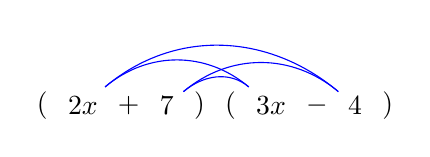
\begin{tikzpicture}
\node(AP1)                       {$($};
\node(A1)   [right=.01cm of AP1]  {$2x$};
\node(AP)   [right=.01cm of A1]   {$+$};
\node(A2)   [right=.01cm of AP]   {$7$};
\node(AP2)  [right=.01cm of A2]   {$)$};
\node(BP1)  [right=.01cm of AP2]  {$($};
\node(B1)   [right=.01cm of BP1]  {$3x$};
\node(BP)   [right=.01cm of B1]   {$-$};
\node(B2)   [right=.01cm of BP]   {$4$};
\node(BP2)  [right=.01cm of B2]   {$)$};
\foreach \x in {1,2}
\foreach \y in {1,2} {
\draw[blue] (A\x) to[out=40,in=140] (B\y);
}
\end{tikzpicture}    
\end{center}
For each line we have a multiplication pair. This lead us to the following
\begin{align*}
(2x+7)(3x-4)&=(2x)(3x)+(2x)(-4)+(7)(3x)+(7)(-4)\\
&=6x^2-8x+21x-28\\
&=6x^2{\color{blue}-8x+21x}-28\\
&=6x^2+13x-28
\end{align*}
\answer{$6x^2+13x-28$}
\end{solution}
\vspace{0.5em}

\begin{exercise}
Simplify the following:
\[
(5x+2)^2
\]
\end{exercise}
\begin{solution}[2in]
Recall that $a^2=a\cdot a$, so
\begin{align*}
(5x+2)^2&=(5x+2)(5x+2)\\
&=(5x)(5x)+(5x)(2)+(2)(5x)+(2)(2)\\
&=25x^2+10x+10x+4\\
&=25x^2+20x+4
\end{align*}
\answer{$25x^2+20x+4$}
\begin{note}
We call this type of polynomial a \emph{perfect square trinomial}.
\end{note}
\end{solution}
\vspace{0.5em}
\begin{exercise}
Multiply the following binomials:
\[
(3x+1)(3x-1)
\]
\end{exercise}
\begin{solution}[2in]
Again we will use the F.O.I.L. method:
\begin{align*}
(3x+1)(3x-1)&=(3x)(3x)+(3x)(-1)+(1)(3x)+(1)(-1)\\
&=9x^2-3x+3x-1\\
&=9x^2-1
\end{align*}
\answer{$9x^2-1$}
\begin{note}
We call this type of binomial a \emph{difference of squares} because
it is of the form $a^2-b^2$.
\end{note}
\end{solution}
\vspace{0.5em}
\ifprintanswers\else\newpage\fi
\begin{exercise}
Multiply the following:
\[
(5x-7)(6x^2-5x+3)
\]
\end{exercise}
\begin{solution}[2in]
While there are more terms, we are simply going to extend the idea of F.O.I.L. like so:
\begin{center}
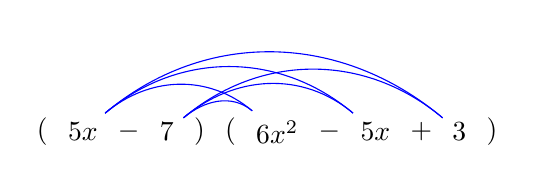
\begin{tikzpicture}
\node(AP1)                          {$($};
\node(A1)   [right=.01cm of AP1]    {$5x$};
\node(AP)   [right=.01cm of A1]     {$-$};
\node(A2)   [right=.01cm of AP]     {$7$};
\node(AP2)  [right=.01cm of A2]     {$)$};
\node(BP1)  [right=.01cm of AP2]    {$($};
\node(B1)   [right=.01cm of BP1]    {$6x^2$};
\node(BS1)  [right=.01cm of B1]     {$-$};
\node(B2)   [right=.01cm of BS1]    {$5x$};
\node(BS2)  [right=.01cm of B2]     {$+$};
\node(B3)   [right=.01cm of BS2]    {$3$};
\node(BP2)  [right=.01cm of B3]     {$)$};
\foreach \x in {1,2}
\foreach \y in {1,2,3} {
\draw[blue] (A\x) to[out=40,in=140] (B\y);
}
\end{tikzpicture}    
\end{center}
Again for each of the lines we get a multiplication pair. This leads us to
\begin{align*}
(5x-7)(6x^2-5x+3)&=(5x)(6x^2)+(5x)(-5x)+(5x)(3)+(-7)(6x^2)+(-7)(-5x)+(-7)(3)\\
&=30x^3-25x^2+15x-42x^2+35x-21\\
&=30x^3{\color{red}-25x^2}{\color{blue}+15x}{\color{red}-42x^2}{\color{blue}+35x}-21\\
&=30x^3-67x^2+50x-21
\end{align*}
\answer{$30x^3-67x^2+50x-21$}
\end{solution}
\vspace{0.5em}

\begin{exercise}
Multiply the following:
\[
(3x^2-4)(6x^2-7x+2)
\]
\end{exercise}
\begin{solution}[2in]
Just like the previous problem we have
\begin{align*}
(3x^2-4)(6x^2-7x+2)&=(3x^2)(6x^2)+(3x^2)(-7x)+(3x^2)(2)+(-4)(6x^2)+(-4)(-7x)+(-4)(2)\\
&=18x^4-21x^3+6x^2-24x^2+28x-8\\
&=18x^4-21x^3{\color{blue}+6x^2-24x^2}+28x-8\\
&=18x^4-21x^3-18x^2+28x-8
\end{align*}
\answer{$18x^4-21x^3-18x^2+28x-8$}
\end{solution}
\vspace{0.5em}

\ifprintanswers
\newpage
\fi

\subsection{Factoring}

\subsubsection{Greatest Common Factor}

\begin{definition}\label{def: GCF}
Given a collection of terms, the \emph{Greatest Common Factor} (or \emph{GCF}) is the largest factor
that divides everything in the collection.
\end{definition}

Our process will involve breaking the problem into finding the GCF of the numbers and
the GCF of the variables, and then mulitplying them together.
\vspace{1em}

\begin{fact}
Given two real numbers $a$ and $b$ with $a\leq b$, the GCF of $x^a$ and $x^b$ is \ifprintanswers \underline{$x^a$}
\else \underline{\phantom{========}}\fi
\end{fact}

\ifprintanswers\else\newpage\fi

\begin{exercise}
Find the Greatest Common Factor (GCF) of $8z^5$ and $36z^3$
\end{exercise}
\begin{solution}[2in]
The GCF of $8$ and $36$ is \underline{\phantom{=}$4$\phantom{=}}, and the GCF of $z^5$ and $z^3$
is $z^3$, so this means that the GCF of $8z^5$ and $36z^3$ is $4z^3$.

\answer{$4z^3$}
\end{solution}
\vspace{0.5em}

We can use this to do the most basic type of factoring for polynomials which is to factor out
the GCF of all the terms in the polynomial (if there is one).

\begin{exercise}
Factor out the GCF from
\[
45x^5y^7+33x^3y^3+78x^2y^4
\]
\end{exercise}
\begin{solution}[2in]
We once again break this into 3 pieces.
\begin{itemize}
\item GCF of $45$, $33$, and $78$ is \underline{\phantom{=}$3$\phantom{=}}
\item GCF of $x^5$, $x^3$, and $x^2$ is \underline{\phantom{=}$x^2$\phantom{=}}
\item GCF of $y^7$, $y^3$, and $y^4$ is \underline{\phantom{=}$y^3$\phantom{=}}
\end{itemize}
This means that the GCF of $45x^5y^7$, $33x^3y^3$, and $78x^2y^4$ is $3x^2y^3$. We now
want to factor this out of each term and write what is left that is $3x^2y^3(\cdots)$.

This gives us the following:
\[
45x^5y^7+33x^3y^3+78x^2y^4=3x^2y^3(15x^3y^4+11x+26y)
\]
\answer{$3x^2y^3(15x^3y^4+11x+26y)$}
\end{solution}
\vspace{0.5em}

\begin{exercise}
Factor out the GCF from
\[
87x^8y^3+18x^5y+21x^4y^2
\]
\end{exercise}
\begin{solution}[2in]
We once again break this into 3 pieces.
\begin{itemize}
\item GCF of $87$, $18$, and $21$ is \underline{\phantom{=}$3$\phantom{=}}
\item GCF of $x^8$, $x^5$, and $x^4$ is \underline{\phantom{=}$x^4$\phantom{=}}
\item GCF of $y^3$, $y$, and $y^2$ is \underline{\phantom{=}$y$\phantom{=}}
\end{itemize}
This means that the GCF of $87x^8y^3$, $18x^5y$, $21x^4y^2$ is $3x^4y$. We now
want to factor this out of each term as follows:
\[
87x^8y^3+18x^5y+21x^4y^2=3x^4y(29x^4y^2+6x+7y)
\]
\answer{$3x^4y(29x^4y^2+6x+7y)$}
\end{solution}

\subsubsection{Factoring by grouping}
When there is not a \hyperref[def: GCF]{GCF} to factor out, we need different methods to
factor polynomials. We will mainly focus on factoring trinomials and specifically
quadratics which are of the form $ax^2+bx+c$.

\subsubsection*{Leading coefficient $a=1$}

In this situation, our quadratic will look like $x^2+bx+c$. Our method for factoring
these will be to find two numbers $m$ and $n$ such that $m+n=b$ and $m\cdot n=c$.
We'll see what we do with this $m$ and $n$ in the following exercise.

% \begin{fact}
% If we multiply $(x+m)(x+n)$ we get the following
% \[
% (x+m)(x+n)
% =\ifprintanswers\underline{\phantom{=}1\phantom{=}}\else\underline{\phantom{===}}\fi x^2
% +\ifprintanswers\underline{\phantom{=}(m+n)\phantom{=}}\else\underline{\phantom{====}}\fi x
% +\ifprintanswers\underline{\phantom{=}mn\phantom{=}}\else\underline{\phantom{====}}\fi
% \]
% \end{fact}

% Based on this fact we will try to find such an $m$ and $n$

\begin{exercise}
Factor the following polynomial
\[
y^2+6y+5
\]
\end{exercise}
\begin{solution}[2.5in]
As stated above, our goal is to find an $m$ and $n$ such $m\cdot n=5$ and $m+n=6$.
The values of $m=1$ and $n=5$, satisfy those requirements. This will allow
us to rewrite $6y$ into $y+5y$ which gives us:
\begin{align*}
y^2+6y+5&=y^2+y+5y+5\\
\intertext{We now group the first two terms with the last two terms.}
&=(y^2+y)+(5y+5)\\
\intertext{We now factor out the GCF from each.}
&=y(y+1)+5(y+1)\\
\intertext{We now factor out the $(y+1)$.}
&=(y+1)(y+5)
\end{align*}
\answer{$(y+1)(y+5)$}
\end{solution}
\vspace{0.5em}

\begin{exercise}
Factor the following polynomial
\[
x^2+8x-20
\]
\end{exercise}
\begin{solution}[2.5in]
For this problem we need find an $m$ and $n$ such $m\cdot n=-20$ and $m+n=8$.
The values of $m=10$ and $n=-2$ work, and will allow
us to rewrite $8x$ into $10x-2x$. This gives us:
\begin{align*}
x^2+8x-20&=x^2+10x-2x-20\\
\intertext{We now group the first two terms with the last two terms.}
&=(x^2+10x)+(-2x-20)\\
\intertext{We now factor out the GCF from each.}
&=x(x+10)-2(x+10)\\
\intertext{We now factor out the $(x+10)$.}
&=(x+10)(x-2)
\end{align*}
\answer{$(x+10)(x-2)$}
\end{solution}
\vspace{0.5em}

\ifprintanswers
\newpage
\fi
\subsubsection*{Leading coefficient $a\neq1$}

The process for $a\neq1$ turns out to be almost exactly the same. We still
want an $m$ and $n$ such that $m+n=b$, but now we have $m\cdot n=a\cdot c$.

\begin{exercise}
Factor the following polynomial:
\[
4x^2+19x+21
\]
\end{exercise}
\begin{solution}[3in]
For this problem we want $m+n=19$ and $m\cdot n=4\cdot21=84$. The values of
$m=12$ and $n=7$ will work, so breaking $19x$ in $12x+7x$ gets us the following:
\begin{align*}
4x^2+19x+21&=4x^2+12x+7x+21\\
&=(4x^2+12x)+(7x+21)\\
&=4x(x+3)+7(x+3)\\
&=(x+3)(4x+7)
\end{align*}
\answer{$(x+3)(4x+7)$}
\end{solution}
\vspace{0.5em}
\ifprintanswers
\begin{note}
You will notice that this is actually the same as the earlier case. Because
if $a=1$ then $a\cdot c=1\cdot c=c$.
\end{note}
\fi

\begin{exercise}
Factor the following polynomial:
\[
-6x^2+17x-7
\]
\end{exercise}
\begin{solution}[3in]
For this problem we want $m+n=17$ and $m\cdot n=-6\cdot-7=42$. The values of
$m=14$ and $n=3$ will work, so breaking $17x$ in $14x+3x$ gives us the following:
\begin{align*}
-6x^2+17x-7&=-6x^2+14x+3x-7\\
&=(-6x^2+14x)+(3x+-7)\\
&=-2x(3x-7)+1(3x-7)\\
&=(3x-7)(-2x+1)
\end{align*}
\answer{$(3x-7)(-2x+1)$}
\end{solution}
\vspace{0.5em}

\subsubsection{Special polynomials}

\begin{definition}\label{def: perfect square binomials}
The following is called a \emph{perfect square trinomial} and factors as follows:
\[
A^2+2AB+B^2=\underline{\phantom{=}\ifprintanswers (A+B)^2\else\phantom{===}\fi\phantom{=}}
\]
Similarly,
\[
A^2-2AB+B^2=\underline{\phantom{=}\ifprintanswers (A-B)^2\else\phantom{===}\fi\phantom{=}}
\]
\end{definition}
\vspace{0.5em}

\begin{exercise}
Factor the following polynomial:
\[
16x^2+24x+9
\]
\end{exercise}
\begin{solution}[3in]
We notice that $16x^2$ and $9$ are perfect squares.
\end{solution}
\vspace{0.5em}

\begin{exercise}
Factor the following polynomial:
\[
25x^2-90x+81
\]
\end{exercise}
\begin{solution}[3in]

\end{solution}
\vspace{0.5em}

\begin{definition}\label{def: diff of squares}
The following is called a \emph{difference of squares} and factors as follows:
\[
A^2-B^2=(A+B)(A-B)
\]
\end{definition}

\begin{exercise}
Factor the following:
\[
x^2-9
\]
\end{exercise}
\begin{solution}[2in]

\end{solution}
\vspace{0.5em}

\begin{exercise}
Factor the following:
\[
16x^2-25y^2
\]
\end{exercise}
\begin{solution}[2in]

\end{solution}
\vspace{0.5em}

\begin{exercise}
Factor the following:
\[
16x^4-81
\]
\end{exercise}
\begin{solution}[2in]

\end{solution}
\vspace{0.5em}

\renewcommand{\thesection}{\arabic{section}}
\setcounter{section}{0}

\section{Linear \& Rational Equations}

\subsection{Linear equations}

\begin{definition}\label{def: linear equation}
An equation in one variable is called a \emph{linear equation} if the
highest power of the variable is \blank{$x$}{====}
\end{definition}

\subsubsection{Determining type}

When dealing with any type of equation, they come in 3 forms.
\begin{enumerate}[1)]
\item Identity: An equation that is always true no matter the value of the variable.

\quad Examples:\underline{\phantom{=}\ifprintanswers$3=3$, $x=x$, $2x+1=2x+1$\else\phantom{=================}\fi\phantom{=}}

\item Inconsistent: An equation that is always false no matter the value of the variable.

\quad Examples:\underline{\phantom{=}\ifprintanswers$3=4$, $7=5$, $0=2$\else\phantom{=================}\fi\phantom{=}}

\item Conditional: An equation that is only true for specific values of the variable.

\quad Examples:\underline{\phantom{=}\ifprintanswers$x=2$, $7x=5$, $2x+1=5$\else\phantom{=================}\fi\phantom{=}}
\end{enumerate}

\begin{exercise}
Determine what type of equation, and solve if it is consistent.
\[
9-10x+7x=2-3x+6
\]
\end{exercise}
\begin{solution}[1.5in]

\end{solution}
\vspace{0.5em}

\begin{exercise}
Determine what type of equation, and solve if it is consistent.
\[
9x-2-2x=5-7+7x
\]
\end{exercise}
\begin{solution}[2in]

\end{solution}
\vspace{0.5em}

\begin{exercise}
Determine what type of equation, and solve if it is consistent.
\[
3x-1=11
\]
\end{exercise}
\begin{solution}[2in]

\end{solution}
\vspace{0.5em}

\subsubsection{Solving linear equations}

\begin{exercise}
Solve the following linear equation:
\[
6(x+2)-2=-6-3(x-5)
\]
\end{exercise}
\begin{solution}[2in]

\end{solution}
\vspace{0.5em}

\begin{definition}\label{def: LCD}
Given a collection of denominators, the \emph{Least Common Denominator} (or \emph{LCD})
is the smallest term that is divisible by all of the denominators.
\end{definition}

\vspace{0.5em}

\begin{note}
The LCD needs to be at least as big as the largest denominator. This may seem
strange since it is the ``Least'' which we usually associate with smallest.
\end{note}

\newpage

\begin{exercise}
Solve the following linear equation:
\[
\frac{9x}{4}+\frac{5}{2}=\frac{-1}{2}
\]
\end{exercise}
\begin{solution}[2in]

\end{solution}
\vspace{0.5em}

\subsection{Rational Equations}

\begin{definition}
A \emph{rational equation} is an equation that involves variables in denominators.
\end{definition}

When solving rational equations, we will follow a similar process to the previous problem
by using the Least Common Denominator. It will involve denominators with variables.

\begin{fact}
Given two real numbers $a$ and $b$ with $a\leq b$, the LCD of $x^a$ and $x^b$
is \blank{$x^b$}{====}
\end{fact}

\begin{exercise}
Solve the following equation:
\[
\frac{7}{2x}+\frac{5}{6x}=\frac{7}{4}
\]
\end{exercise}
\begin{solution}[3in]

\end{solution}
\vspace{0.5em}

\begin{exercise}
Solve the following equation:
\[
-\frac{2}{3x}-\frac{5}{6x}=\frac{3}{2}
\]
\end{exercise}
\begin{solution}[3.5in]

\end{solution}
\vspace{0.5em}

\begin{exercise}
Solve the following equation:
\[
\frac{-7}{x}=\frac{-5}{x+4}
\]
\end{exercise}
\begin{solution}[3.5in]

\end{solution}
\vspace{0.5em}

\begin{exercise}
Solve the following equation:
\[
\frac{-1}{x+3}-\frac{6}{x+1}=\frac{-2}{x^2+4x+3}
\]
\end{exercise}
\begin{solution}[3.5in]

\end{solution}
\vspace{0.5em}

\begin{exercise}
Solve the following equation:
\[
\frac{-3}{x-2}+\frac{5}{x-4}=\frac{-1}{x^2-6x+8}
\]
\end{exercise}
\begin{solution}[3.5in]

\end{solution}
\vspace{0.5em}

\newpage

\section{Complex Numbers}

\subsection{The Basics}

\ifprintanswers
\begin{center}
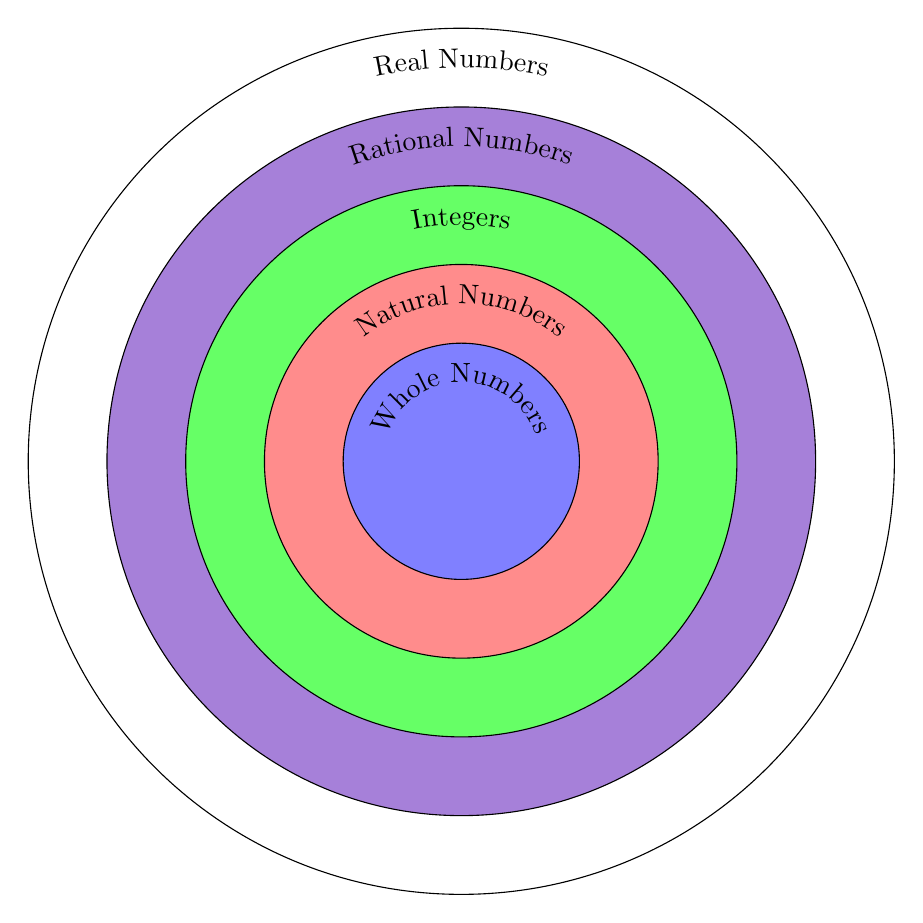
\begin{tikzpicture}
\coordinate (O) at (0,0);

\draw (O) circle (5.5);
\draw[fill=blue!70!red!50!white] (O) circle (4.5);
\draw[fill=green!60] (O) circle (3.5);
\draw[fill=red!45] (O) circle (2.5);
\draw[fill=blue!50] (O) circle (1.5);

\draw[decoration={text along path,reverse path,text align={align=center},text={Whole Numbers}},decorate] (1,0) arc (0:180:1);
\draw[decoration={text along path,reverse path,text align={align=center},text={Natural Numbers}},decorate] (2,0) arc (0:180:2);
\draw[decoration={text along path,reverse path,text align={align=center},text={Integers}},decorate] (3,0) arc (0:180:3);
\draw[decoration={text along path,reverse path,text align={align=center},text={Rational Numbers}},decorate] (4,0) arc (0:180:4);
\draw[decoration={text along path,reverse path,text align={align=center},text={Real Numbers}},decorate] (5,0) arc (0:180:5);

\end{tikzpicture}
\end{center}
\else
\begin{center}
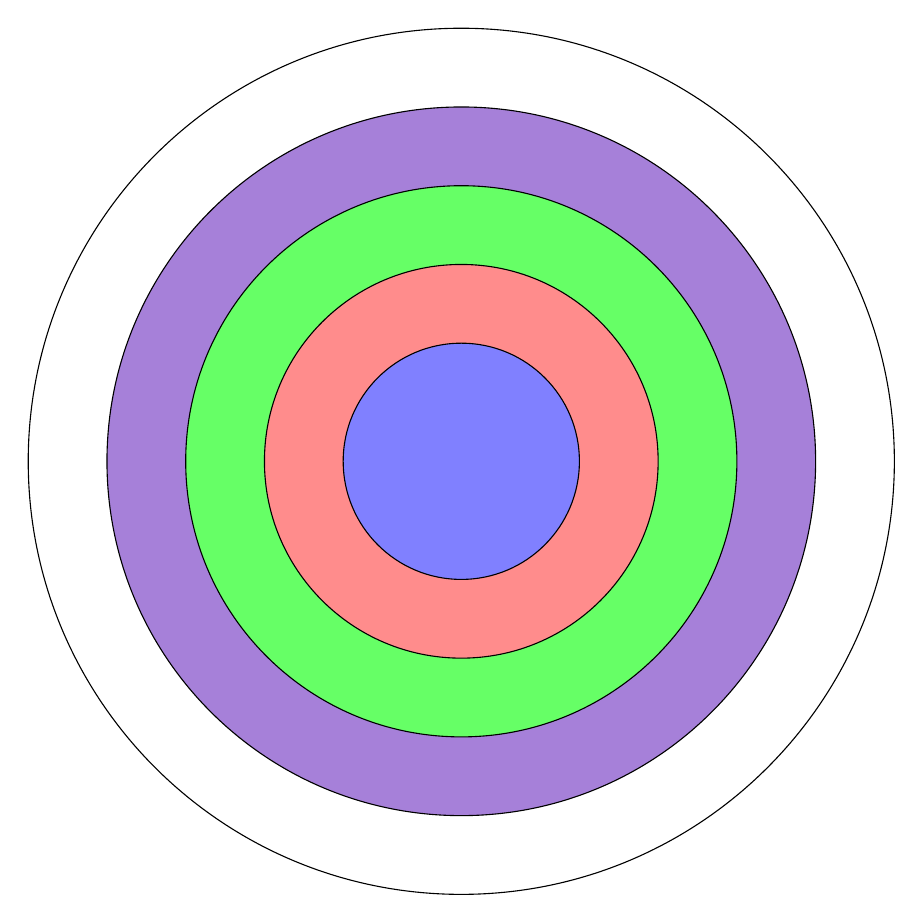
\begin{tikzpicture}
\coordinate (O) at (0,0);

\draw (O) circle (5.5);
\draw[fill=blue!70!red!50!white] (O) circle (4.5);
\draw[fill=green!60] (O) circle (3.5);
\draw[fill=red!45] (O) circle (2.5);
\draw[fill=blue!50] (O) circle (1.5);
\end{tikzpicture}
\end{center}
\fi

\begin{ques}
How do we deal with $\sqrt{-1}$?
\end{ques}

\begin{definition}
The \emph{imaginary constant} is defined to be $i=\sqrt{-1}$
\end{definition}

\begin{note}
This will now allow us to deal with square roots with negative values. If $n>0$, then
\[
\sqrt{-n}=\blank{=\sqrt{-1\cdot n}=\sqrt{-1}\sqrt{n}=i\sqrt{n}}{=\sqrt{-1\cdot n}=\sqrt{-1}\sqrt{n}=i\sqrt{n}}
\]
\end{note}
\begin{exercise}
Simplify $\sqrt{-75}$.
\end{exercise}
\begin{solution}[2in]

\end{solution}
\vspace{0.5em}

\begin{note}
We can simplify powers of $i$ as follows:
\begin{align*}
i&=i\\
i^2&=\blank{(\sqrt{-1})^2=-1}{===========}\\
i^3&=\blank{(i^2\cdot i=-i}{===========}\\
i^4&=\blank{i^2\cdot i^2=(-1)(-1)=1}{===========}\\
i^5&=\blank{i^4\cdot i=1\cdot i=i}{===========}\\
i^6&=\blank{-1}{===========}\\
i^7&=\blank{-i}{===========}\\
&\vdots
\end{align*}
\ifprintanswers This pattern repeats forever.\fi
\end{note}

\begin{exercise}
Simplify $i^{62}$
\end{exercise}
\begin{solution}[2in]

\end{solution}
\vspace{0.5em}

\begin{exercise}
Simplify $i^{19}$
\end{exercise}
\begin{solution}[2in]

\end{solution}
\vspace{0.5em}

\begin{note}
We can also continue the pattern in reverse to get negative powers of $i$:
\begin{align*}
i^0&=\blank{1}{===========}\\
i^{-1}&=\blank{-i}{===========}\\
i^{-2}&=\blank{-1}{===========}\\
i^{-3}&=\blank{i}{===========}\\
&\vdots
\end{align*}
\end{note}

\begin{definition}\label{def: Complex number}
The \emph{complex numbers} (denoted by $\mathbb{C}$) is the set of all
numbers of the form $a+bi$ where $a$ and $b$ are real numbers and $i$
is the imaginary constant.

We call $a+bi$ the standard form of a complex number, calling $a$ the real part
and $b$ the imaginary part.
\end{definition}

\subsection{Addition \& Subtraction}

\begin{exercise}
Compute the following:
\[
(3+2i)+(4-7i)
\]
\end{exercise}
\begin{solution}[1.5in]

\end{solution}
\vspace{0.5em}

\begin{exercise}
Compute the following:
\[
(5+7i)-(-3+2i)
\]
\end{exercise}
\begin{solution}[1.5in]

\end{solution}
\vspace{0.5em}

\subsection{Multiplication}

\begin{exercise}
Compute the following:
\[
3(7-5i)
\]
\end{exercise}
\begin{solution}[2in]

\end{solution}
\vspace{0.5em}

\begin{exercise}
Compute the following:
\[
7i(2+4i)
\]
\end{exercise}
\begin{solution}[2in]

\end{solution}
\vspace{0.5em}

\begin{exercise}
Compute the following:
\[
(-3+7i)(2+5i)
\]
\end{exercise}
\begin{solution}[2in]

\end{solution}
\vspace{0.5em}

\begin{exercise}
Compute the following:
\[
(3+2i)(3-2i)
\]
\end{exercise}
\begin{solution}[3in]

\end{solution}
\vspace{0.5em}

\begin{definition}\label{def: complex conjugates}
The two complex numbers $a+bi$ and $a-bi$ are called \emph{complex conjugates}.
Their product is always $a^2+b^2$ which is real.
\end{definition}

\subsection{Division}

In order to divide complex numbers we will need to use the complex conjugate of
the complex number we are dividing by (the denominator).

\begin{example}
Give the complex conjugates for the following complex numbers:
\begin{itemize}
    \item $5-2i\longleftrightarrow\blank{5+2i}{=====}$
    \vspace{0.5em}
    \item $7+11i\longleftrightarrow\blank{7-11i}{=====}$
    \vspace{0.5em}
    \item $-4-2i\longleftrightarrow\blank{-4+2i}{=====}$
\end{itemize}
\end{example}

\vspace{0.5em}

\begin{exercise}
Divide the following and write your answer in standard form.
\[
\frac{16+22i}{3+i}
\]
\end{exercise}
\begin{solution}[2in]

\end{solution}
\vspace{0.5em}

\newpage

\begin{exercise}
Divide the following and write your answer in standard form.
\[
(17+5i)\div(-2+i)
\]
\end{exercise}
\begin{solution}[3.5in]

\end{solution}
\vspace{0.5em}

\section{Solving Quadratic Equations}

\subsection{Solving by Factoring}

\begin{fact}[The Zero Product Rule]
If $AB=0$, then \blank{$A=0$ or $B=0$}{=========}
\end{fact}

\begin{exercise}
Solve the following for $x$:
\[
x^2+4x-21=0
\]
\end{exercise}
\begin{solution}[2in]

\end{solution}
\vspace{0.5em}

\newpage

\begin{exercise}
Solve the following for $y$:
\[
y^2+8y+12=0
\]
\end{exercise}
\begin{solution}[3.5in]

\end{solution}
\vspace{0.5em}

\begin{exercise}
Solve the following for $x$:
\[
9x^2-26x-3=0
\]
\end{exercise}
\begin{solution}[3.5in]

\end{solution}
\vspace{0.5em}

\subsubsection{The Square Root Property}

\begin{exercise}
Solve $x^2=36$ for $x$.
\end{exercise}
\begin{solution}[1.5in]

\end{solution}

\begin{exercise}
Solve $x^2=81$ for $x$.
\end{exercise}
\begin{solution}[1.5in]

\end{solution}

\subsection{Completing the Square}

This will be using the square root property from above and perfect square trinomials
(see Definition \ref{def: perfect square binomials}). We will change our quadratics as
perfect square trinomials, so that we can take a square root to simplify the problem.

\begin{exercise}
If $x^2+4x-45=0$, solve for $x$.
\end{exercise}
\begin{solution}[2in]

\end{solution}
\vspace{0.5em}

\newpage

\begin{exercise}
If $x^2-12x+11=0$, solve for $x$.
\end{exercise}
\begin{solution}[2in]

\end{solution}
\vspace{0.5em}

\subsection{The Quadratic Formula}

Now completing the square works to solve any quadratic equation, but what if we
tried to complete the square on the general quadratic?

\begin{example}
If $ax^2+bx+c=0$, solve for $x$.
\end{example}
\begin{solution}[3in]

\end{solution}

\newpage

\begin{prop}[The Quadratic Formula]\label{prop: Quadratic Formula}
If $ax^2+bx+c=0$, then
\[
x=\ifprintanswers\frac{-b\pm\sqrt{b^2-4ac}}{2a}\else\phantom{\frac{-b\pm\sqrt{b^2-4ac}}{2a}}\fi
\]
\end{prop}
\vspace{0.5em}

\begin{definition}\label{def: discriminant}
For a quadratic equation $ax^2+bx+c=0$, the \emph{discriminant} is
$b^2-4ac$, and it tells us about the types of
solutions to said equation.

There are 3 (really 4) cases:
\begin{itemize}
    \item $b^2-4ac<0\Rightarrow$ \blank{2 complex solutions}{2 complex solutions}
    \item $b^2-4ac=0\Rightarrow$ \blank{1 rational solution}{1 rational solution}
    \item $b^2-4ac>0$ and
    \begin{itemize}
        \item it IS a perfect square $\Rightarrow$ \blank{2 (distinct) rational solutions}{2 (distinct rational solutions}
        \item it IS NOT a perfect square $\Rightarrow$ \blank{2 irrational solutions}{2 irrational solutions}
    \end{itemize}
\end{itemize}
\end{definition}
\vspace{0.5em}

\begin{exercise}
Find the discriminant and solve $-4x^2+5x+3=0$.
\end{exercise}
\begin{solution}[3in]

\end{solution}
\vspace{0.5em}

\newpage

\begin{exercise}
Find the discriminant and solve $4n^2-20n+25=0$.
\end{exercise}
\begin{solution}[3in]

\end{solution}
\vspace{0.5em}

\section{More Equations and Some Applications}
\subsection{Using the Greatest Common Factor}

\begin{exercise}
Solve $4x^4=16x^2$
\end{exercise}
\begin{solution}[2in]

\end{solution}
\vspace{0.5em}

\begin{exercise}
Solve $9x^4=81x^2$
\end{exercise}
\begin{solution}[1.5in]

\end{solution}
\vspace{0.5em}

\subsection{Factoring by Grouping}
\begin{exercise}
Solve $x^3-5x^2-4x+20=0$.
\end{exercise}
\begin{solution}[2.2in]

\end{solution}
\vspace{0.5em}

\begin{exercise}
Solve $x^3-8x^2-9x+72=0$.
\end{exercise}
\begin{solution}[2.2in]

\end{solution}
\vspace{0.5em}

\begin{exercise}
Solve $x^3+7x^2-x-7=0$.
\end{exercise}
\begin{solution}[2.2in]

\end{solution}
\vspace{0.5em}

\newpage
\subsection{Polynomials in Quadratic Form}

\begin{exercise}
Solve $(x-5)^2+(x-5)-2=0$.
\end{exercise}
\begin{solution}[4in]

\end{solution}
\vspace{0.5em}

\begin{exercise}
Solve $(x-7)^2-7(x-7)+10=0$.
\end{exercise}
\begin{solution}[3in]

\end{solution}
\vspace{0.5em}

\newpage
\subsection{Absolute Value Equations}
\begin{definition}\label{def: absolute value}
The \emph{absolute value} of a number $n$, written $\vert n\vert$, is the
distance from $n$ to $0$ on the number line (i.e. it is the positive version of $n$).
\end{definition}

\begin{example}
If $\vert x\vert=5$, then either $x=5$ or $x=-5$
\end{example}

This means that absolute value equations are just two problems in one. A positive equation and a negative equation.

\begin{exercise}
If $\vert-12x-7\vert-8=2$, solve for $x$.
\end{exercise}
\begin{solution}[3.5in]

\end{solution}
\vspace{0.5em}

\begin{exercise}
Solve $2\vert x+1\vert+7=10$ for $x$.
\end{exercise}
\begin{solution}[3in]

\end{solution}
\vspace{0.5em}

\begin{exercise}
Solve the following for $x$:
\[
\vert 3x-5\vert-11=-9
\]
\end{exercise}
\begin{solution}[3in]

\end{solution}
\vspace{0.5em}

\subsection{Radical Equations}

Our goal will be to get rid of the radical in the problem.

\begin{exercise}
Solve the following for $x$:
\[
\sqrt{8x-23}+2=x
\]
\end{exercise}
\begin{solution}[4in]

\end{solution}

\begin{exercise}
Solve:
\[
\sqrt{-2x+8}=x
\]
\end{exercise}
\begin{solution}[3in]

\end{solution}
\vspace{0.5em}

\begin{exercise}
Solve:
\[
\sqrt{-x+4}+\sqrt{5x+1}=3
\]
\end{exercise}
\begin{solution}[4in]

\end{solution}

\newpage

\begin{exercise}
Solve:
\[
\sqrt{-2x+2}+\sqrt{x+2}=-3
\]
\end{exercise}
\begin{solution}[2in]

\end{solution}
\vspace{0.5em}

\subsection{Rational Exponent Equations}

Recall that the square root is the same as the \blank{$1/2$}{1/2} power, so
in general we take
\[
\Big(\big(~~\big)^{m/n}\Big)^{\blank{n}{n}/\blank{m}{m}}
\]

\begin{exercise}
Solve $x^{7/6}=128$ for $x$.
\end{exercise}
\begin{solution}[2in]

\end{solution}
\vspace{0.5em}

\begin{exercise}
Find $x$ when $\dl x^{-3/2}=\frac{1}{125}$
\end{exercise}
\begin{solution}[2in]

\end{solution}
\vspace{0.5em}

\begin{exercise}
Solve for $x$ when $\dl (x-1)^{-4/3}=\frac{1}{81}$
\end{exercise}
\begin{solution}[3.5in]

\end{solution}
\vspace{0.5em}

\begin{exercise}
Solve the following for $x$:
\[
7x^4-189x^{13/4}=0
\]
\end{exercise}
\begin{solution}[4in]

\end{solution}
\vspace{0.5em}
\begin{exercise}
Solve the following for $x$:
\[
4x^3-36x^{7/3}=0
\]
\end{exercise}
\begin{solution}[2in]

\end{solution}
\vspace{0.5em}

\subsection{More Rational Equations}

\begin{note}
We still need to check what makes our denominators equal to 0
\end{note}
\vspace{0.5em}

\begin{exercise}
If $\dl \frac{6x+5}{x+2}-\frac{1}{x}=-\frac{2}{x^2+2x}$, find $x$.
\end{exercise}
\begin{solution}[4in]

\end{solution}
\vspace{0.5em}

\newpage

\section{Linear, Compound, and Absolute Value Inequalities}\label{sec: linear and absolute inequalities}

We need a shared language to discuss these problems because
the answers are not just single numbers they are sets (or
collections) of numbers like the following:

\begin{example}\label{example: numberline}
The set of all real numbers greater than or equal to 1.

\vspace{0.1in}

\begin{center}
\begin{tikzpicture}
\node(N)                        {$-\infty$};
\node(P)    [right=8cm of N]    {$\infty$};

\draw[>=stealth,black,<->] (N) -- (P);
\end{tikzpicture}
\end{center}
\end{example}

\subsection{Interval Notation}

\[
\begin{tabular}{c|c}
Set Builder Notation & Interval Notation \\
\hline
& \\
$\{x\mid a<x<b\}$ & \blank{$(a,b)$}{$(a,b)$}\\
& \\
$\{x\mid a\le x\le b\}$ & \blank{$[a,b]$}{$[a,b]$} \\
& \\
$\{x\mid a<x\le b\}$ & \blank{$(a,b]$}{$(a,b]$} \\
& \\
$\{x\mid a\le x<b\}$ & \blank{$[a,b)$}{$[a,b)$} \\
& \\
$\{x\mid a\le x\}$ & \blank{$[a,\infty)$}{$[a,\infty)$} \\
& \\
$\{x\mid x<b\}$ & \blank{$(-\infty,b)$}{$(-\infty,b)$} \\
\end{tabular}
\]

\begin{exercise}
Write the number line from Example \ref{example: numberline} in
interval notation.
\end{exercise}
\begin{solution}[1in]

\end{solution}
\vspace{0.5em}

\begin{definition}
\text{}
\begin{itemize}
    \item \blank{$\cup$}{$\cup$} -- denotes the \emph{union} which means ``or''.
    \item \blank{$\cap$}{$\cap$} -- denotes the \emph{intersection} which means ``and''.
\end{itemize}
\end{definition}

\newpage

\begin{exercise}
Use interval notation to express the following:

The set of all real numbers greater than $-1$ and less than $0$.
\end{exercise}
\begin{solution}[2in]

\end{solution}
\vspace{0.5em}

\begin{exercise}
Use interval notation to express the following:

The set of all real numbers greater than $-7$ and less than or equal
to $5$.
\end{exercise}
\begin{solution}[2in]

\end{solution}
\vspace{0.5em}

\begin{exercise}
Use interval notation to express the following:

The set of all real numbers greater than or equal to $4$
or less than $2$.
\end{exercise}
\begin{solution}[2in]

\end{solution}
\vspace{0.5em}

\newpage

\subsection{Properties of Inequalities}

\subsubsection*{Addition Property}
If $a<b$, then for a real number $c$ \blank{$a+c<b+c$}{$a+c<b+c$}.

\subsubsection*{Multiplication Property}
\begin{itemize}
    \item If $a<b$ and $c>0$, then \blank{$ac<bc$}{$ac<bc$}.
    \item If $a<b$ and $c<0$, then \blank{$ac>bc$}{$ac>bc$}.
\end{itemize}

\begin{exercise}
If $x+10\leq4$, solve for $x$.
\end{exercise}
\begin{solution}[1in]

\end{solution}
\vspace{0.5em}

\begin{exercise}
Find $x$ when $-5x-2\leq8$.
\end{exercise}
\begin{solution}[2in]

\end{solution}
\vspace{0.5em}

\begin{exercise}
Solve $-16x+8\geq-9x-13$ for $x$.
\end{exercise}
\begin{solution}[2in]

\end{solution}
\vspace{0.5em}

\newpage

\begin{exercise}
Find $x$ when $-10x+12>-8x-10$.
\end{exercise}
\begin{solution}[2in]

\end{solution}
\vspace{0.5em}

\subsection{Compound Inequalities}

\begin{exercise}
Solve $2x-3\leq4x+3<2x+5$ for $x$.
\end{exercise}
\begin{solution}[2in]

\end{solution}
\vspace{0.5em}

\begin{exercise}
Find $x$ if $-4x-10<-2x-8\leq-4x+10$.
\end{exercise}
\begin{solution}[2in]

\end{solution}
\vspace{0.5em}

\newpage

\subsection{Absolute Value Inequalities}

Recall that absolute values turn one problem into two!

\begin{exercise}
Solve $\vert x-6\vert+2=4$ for $x$.
\end{exercise}
\begin{solution}[2in]

\end{solution}
\vspace{0.5em}

With inequalities we either have an ``and'' or an ``or'' problem.

\begin{note}
Here is a trick to remember:
\begin{itemize}
    \item And -- \blank{Less Th\underline{an}}{Less Th\underline{an}} 
    \item Or -- \blank{Great``or''}{Great``or''}
\end{itemize}
\end{note}

\begin{exercise}
Solve $\vert2x+6\vert<18$ for $x$.
\end{exercise}
\begin{solution}[2in]

\end{solution}
\vspace{0.5em}

\newpage

\begin{exercise}
Solve $-7\vert x+12\vert\leq-14$ for $x$.
\end{exercise}
\begin{solution}[2in]

\end{solution}
\vspace{0.5em}

\begin{exercise}
Solve $2\vert x-12\vert+1\leq23$ for $x$.
\end{exercise}
\begin{solution}[2in]

\end{solution}

\begin{exercise}
Solve $\vert x-5\vert\leq-2$ for $x$.
\end{exercise}
\begin{solution}[2in]

\end{solution}
\vspace{0.5em}

%!TEX root = main.tex
%%% Graphs and Functions
\part{}

\section{The Rectangular Coordinate System}

\subsection{The \texorpdfstring{$x$-$y$}{x-y} plane}

\begin{center}
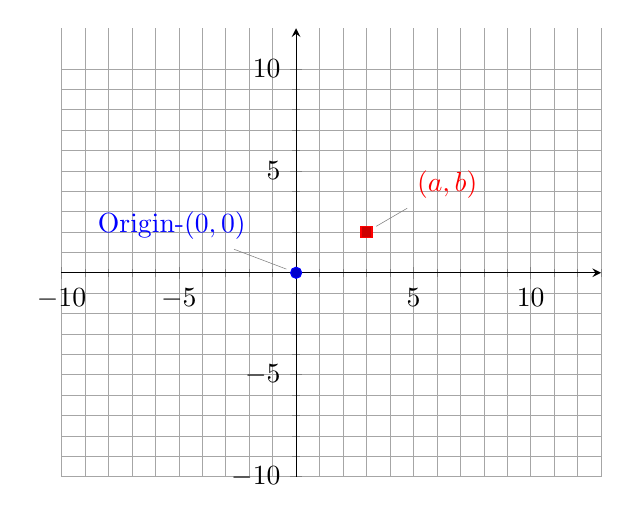
\begin{tikzpicture}
      \begin{axis}%
    [grid=both,
     minor tick num=4,
     grid style={line width=.2pt, draw=gray!70},
     major grid style={line width=.2pt,draw=gray!70},
     axis lines=middle,
     enlargelimits={abs=10}
    ]
    \addplot coordinates {(0,0)} node[pin=150:{Origin-$(0,0)$}]{};
    \addplot coordinates {(3,2)} node[pin=30:{$(a,b)$}]{};
  \end{axis}
\end{tikzpicture}
\end{center}

\begin{exercise}
Find the coordinates of the following points:
\begin{center}
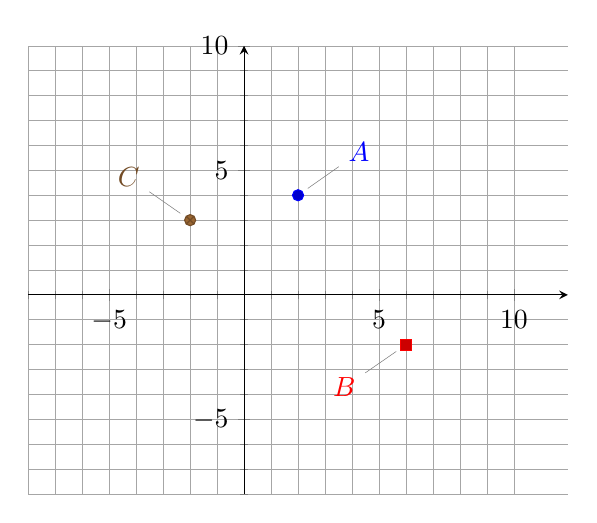
\begin{tikzpicture}
      \begin{axis}%
    [grid=both,
     minor tick num=4,
     grid style={line width=.2pt, draw=gray!70},
     major grid style={line width=.2pt,draw=gray!70},
     axis lines=middle,
     enlargelimits={abs=6}
    ]
    \addplot coordinates {(2,4)} node[pin=30:{$A$}]{};
    \addplot coordinates {(6,-2)} node[pin=210:{$B$}]{};
    \addplot coordinates {(-2,3)} node[pin=150:{$C$}]{};
  \end{axis}
\end{tikzpicture}
\end{center}
\end{exercise}
\begin{solution}[1in]

\end{solution}

\newpage

\subsection{Graphing Lines}

\begin{exercise}
Graph $y=4x-5$ on the $x$-$y$ plane.
\end{exercise}
\ifprintanswers
\else
\begin{center}
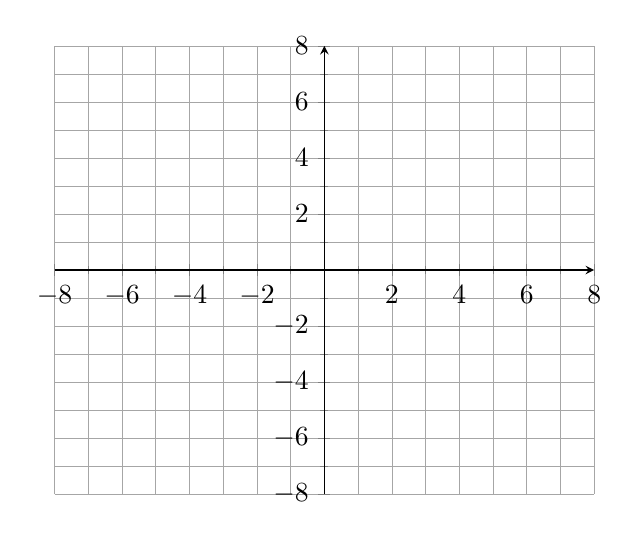
\begin{tikzpicture}
      \begin{axis}%
    [grid=both,
     minor tick num=1,
     grid style={line width=.2pt, draw=gray!70},
     major grid style={line width=.2pt,draw=gray!70},
     xtick={-8,-6,...,6,8},
     ytick={-8,-6,...,6,8},
     xmin=-8, xmax=8,
     ymin=-8, ymax=8,
     axis lines=middle,
     enlargelimits=false
    ]
  \end{axis}
\end{tikzpicture}
\end{center}
\fi
\begin{solution}[2in]

\end{solution}

\begin{exercise}
Graph $y=\frac{4}{3}x-2$ on the $x$-$y$ plane.
\end{exercise}
\ifprintanswers
\else
\begin{center}
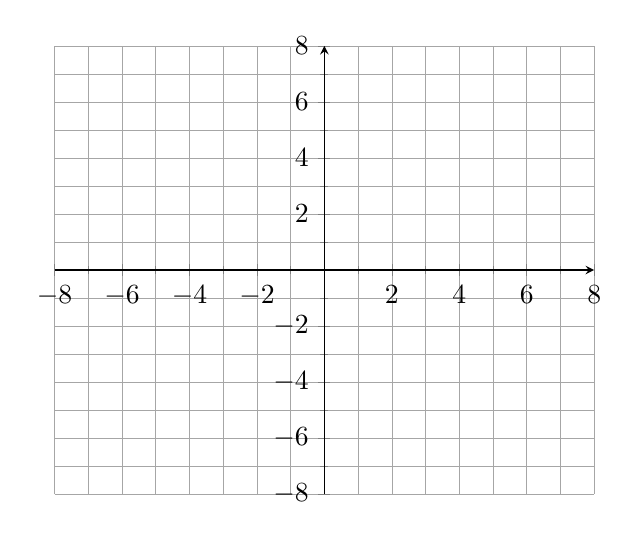
\begin{tikzpicture}
      \begin{axis}%
    [grid=both,
     minor tick num=1,
     grid style={line width=.2pt, draw=gray!70},
     major grid style={line width=.2pt,draw=gray!70},
     xtick={-8,-6,...,6,8},
     ytick={-8,-6,...,6,8},
     xmin=-8, xmax=8,
     ymin=-8, ymax=8,
     axis lines=middle,
     enlargelimits=false
    ]
  \end{axis}
\end{tikzpicture}
\end{center}
\fi
\begin{solution}

\end{solution}

\newpage

\subsection{Distances}

\begin{center}
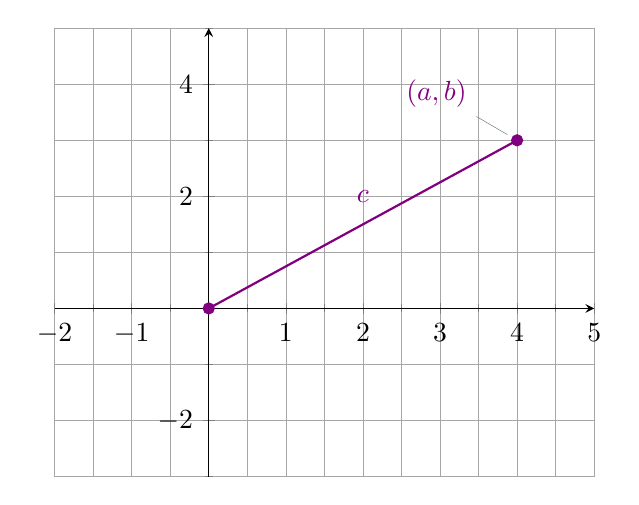
\begin{tikzpicture}
     \begin{axis}%
    [grid=both,
    ymin=-3, ymax=5,
    xmin=-2, xmax=5,
     minor tick num=1,
     grid style={line width=.2pt, draw=gray!70},
     major grid style={line width=.2pt,draw=gray!70},
     axis lines=middle,
     enlargelimits=false
    ]
    \addplot[blue!50!red,only marks] coordinates {(0,0) (4,3)} node[pin=150:{$(a,b)$}]{};
    \addplot[blue!50!red,thick] (0,0) -- (4,3);
    \node[color=blue!50!red] at (2,2) {$c$};
  \end{axis}
\end{tikzpicture}
\end{center}
\begin{ques}
How would we compute the value of $c$ the length of the purple line?
\end{ques}

\subsubsection*{The Pythagorean Theorem}

\begin{theorem}[The Pythagorean Theorem]
Given a right triangle with a hypotenuse of length $c$ and side lengths
$a$ and $b$, then the following holds
\[
\blank{a^2+b^2}{a^2+b^2}=\blank{c^2}{c^2}
\]
\end{theorem}

This means that $c=\blank{\sqrt{a^2+b^2}}{\sqrt{a^2+b^2}}$. Which
is the distance between the points $(0,0)$ \& $(a,b)$.

Looking at it a slightly different way we can say that
\[
c=\blank{\sqrt{(a-0)^2+(b-0)^2}}{(a-0)^2+(b-0)^2}
\]
We can generalize this to the distance between any two points on the plane.

\begin{prop}[The Distance Formula]\label{prop: Distance formula}
Given two points $(x_1,y_1)$ \& $(x_2,y_2)$ in the Cartesian plane, the
distance $D$ between these points is as follows:
\[
D=\blank{\sqrt{(x_2-x_1)^2+(y_2-y_1)^2}}{\sqrt{(x_2-x_1)^2+(y_2-y_1)^2}}
\]
\end{prop}

\begin{exercise}
Find the distance between $(-6,1)$ \& $(5,-1)$.
\end{exercise}
\begin{solution}[2in]

\end{solution}
\vspace{0.5em}

\begin{exercise}
Find the distance between $(2,5)$ \& $(-4,-5)$.
\end{exercise}
\begin{solution}[2in]

\end{solution}
\vspace{0.5em}

\begin{exercise}
Find the distance between $(2,-3)$ \& $(-4,-7)$.
\end{exercise}
\begin{solution}[2in]

\end{solution}
\vspace{0.5em}

\subsection{Midpoints}
\begin{center}
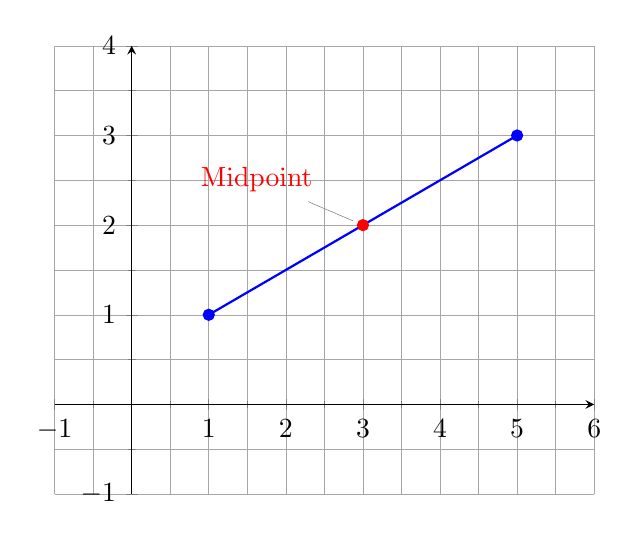
\begin{tikzpicture}
     \begin{axis}%
    [grid=both,
    ymin=-1, ymax=4,
    xmin=-1, xmax=6,
     minor tick num=1,
     grid style={line width=.2pt, draw=gray!70},
     major grid style={line width=.2pt,draw=gray!70},
     axis lines=middle,
     enlargelimits=false
    ]
    \addplot[blue,only marks] coordinates {(1,1) (5,3)};
    \addplot[blue,thick] (1,1) -- (5,3);
    \addplot[red, only marks] coordinates {(3,2)}
    node[pin=150:{Midpoint}]{};
  \end{axis}
\end{tikzpicture}
\end{center}

\begin{definition}
The \emph{midpoint} between two points $(x_1,y_1)$ \& $(x_2,y_2)$
in the Cartesian plane is computed as follows:
\[
\text{Midpoint}=\left(\blank{\frac{x_1+x_2}{2}}{\frac{x_1+x_2}{2}},\blank{\frac{y_1+y_2}{2}}{\frac{y_1+y_2}{2}}\right)
\]
\end{definition}
\vspace{0.5em}

\begin{exercise}
Find the midpoint between $(12,13)$ \& $(-11,7)$.
\end{exercise}
\begin{solution}[2in]

\end{solution}
\vspace{0.5em}

\begin{exercise}
Find the midpoint between $(8,7)$ \& $(12-5)$.
\end{exercise}
\begin{solution}[2in]

\end{solution}
\vspace{0.5em}

\section{Circles}
\begin{center}
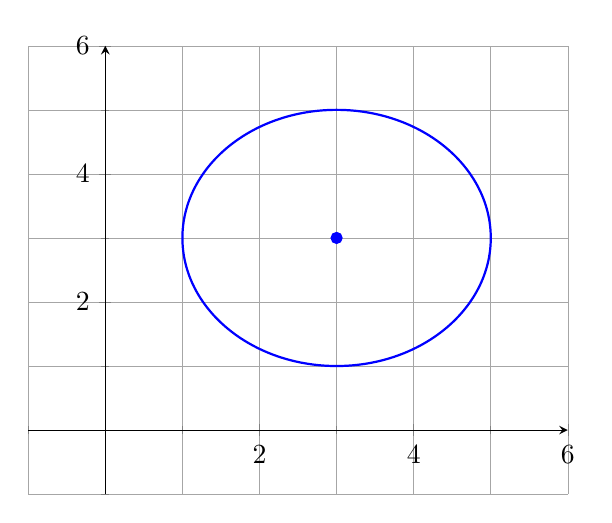
\begin{tikzpicture}
     \begin{axis}%
    [grid=both,
    ymin=-1, ymax=6,
    xmin=-1, xmax=6,
     minor tick num=1,
     xtick = {-2,0,2,...,4,6},
     ytick = {-2,0,2,...,4,6},
     grid style={line width=.2pt, draw=gray!70},
     major grid style={line width=.2pt,draw=gray!70},
     axis lines=middle,
     enlargelimits=false
    ]
    \addplot[blue,only marks] coordinates {(3,3)};
    \draw[color=blue,thick] (axis cs:3,3) circle[radius=2];
  \end{axis}
\end{tikzpicture}
\end{center}

\begin{definition}
A \emph{circle} is a the set of all points $(x,y)$ a distance $r$
from the center $(h,k)$. We call $r$ the \blank{radius}{radius}.
\end{definition}

Using the distance formula (see Proposition
\ref{prop: Distance formula}), we can come up with an equation
for the equation of the a circle as follows
\begin{align*}
\blank{\sqrt{(x-h)^2+(y-k)^2}}{\sqrt{(x-h)^2+(y-k)^2}}&=\blank{r}{r}\\
\blank{(x-h)^2+(y-k)^2}{(x-h)^2+(y-k)^2}&=\blank{r^2}{r^2}\\
\end{align*}

We call this the \emph{standard form of a circle}

\begin{exercise}
Write the following in standard form:
\[
x^2-4x+y^2-2y-31=0
\]
\end{exercise}
\begin{solution}[2in]

\end{solution}
\vspace{0.5em}

\begin{exercise}
Write $2x^2+12x+2y^2+8y-24=0$ in standard form.
\end{exercise}
\begin{solution}[2in]

\end{solution}
\vspace{0.5em}

\newpage

\begin{exercise}
Write the following in standard form:
\[
3x^2-12x+3y^2+6y+3=0
\]
\end{exercise}
\begin{solution}[2in]

\end{solution}
\vspace{0.5em}

\subsection{Graphing circles}

\begin{exercise}
Graph $(x+4)^2+(y+2)^2=16$.
\end{exercise}
\ifprintanswers
\else
\begin{center}
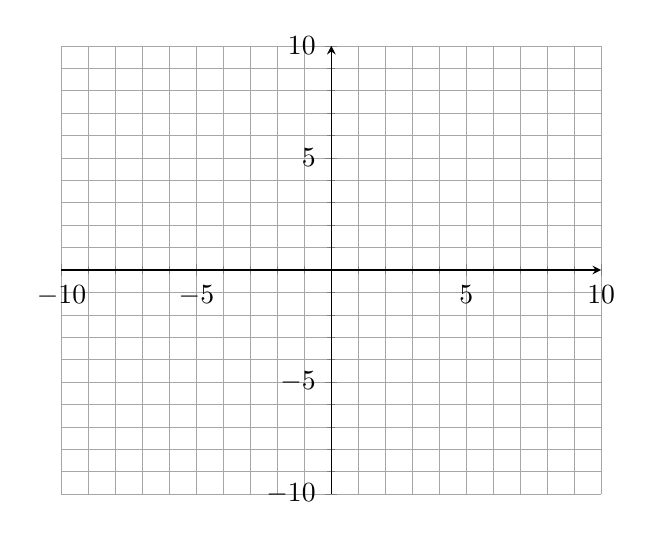
\begin{tikzpicture}
      \begin{axis}%
    [grid=both,
     minor tick num=4,
     grid style={line width=.2pt, draw=gray!70},
     major grid style={line width=.2pt,draw=gray!70},
     xtick={-10,-5,...,5,10},
     ytick={-10,-5,...,5,10},
     xmin=-10, xmax=10,
     ymin=-10, ymax=10,
     axis lines=middle,
     enlargelimits=false
    ]
  \end{axis}
\end{tikzpicture}
\end{center}
\fi
\begin{solution}[2.5in]

\end{solution}

\begin{exercise}
Graph $(x+1)^2+(y-1)^2=4$.
\end{exercise}
\ifprintanswers
\else
\begin{center}
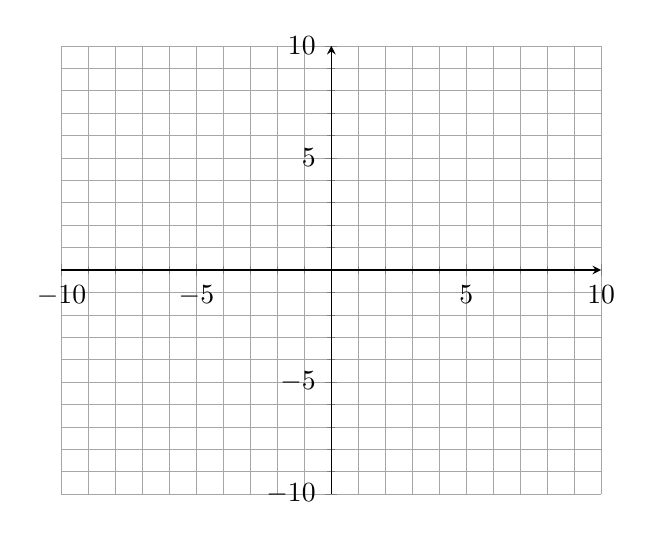
\begin{tikzpicture}
      \begin{axis}%
    [grid=both,
     minor tick num=4,
     grid style={line width=.2pt, draw=gray!70},
     major grid style={line width=.2pt,draw=gray!70},
     xtick={-10,-5,...,5,10},
     ytick={-10,-5,...,5,10},
     xmin=-10, xmax=10,
     ymin=-10, ymax=10,
     axis lines=middle,
     enlargelimits=false
    ]
  \end{axis}
\end{tikzpicture}
\end{center}
\fi
\begin{solution}[2.5in]

\end{solution}

\section{Functions}

\begin{definition}\label{def: relation, domain, range}
A \emph{relation} is any set of order pairs where the \emph{domain}
is the set of \blank{first}{first} values in the ordered pair, and the
\emph{range} is the set of \blank{second}{second} values.
\end{definition}

\begin{exercise}
Find the domain and range of
\[
\{(0,9.1),~(10,6.7),~(20,10.7)\}.
\]
\end{exercise}
\begin{solution}[1.5in]

\end{solution}

\begin{definition}
A \emph{function} is a relation where each element in the domain,
corresponds to exactly one element of the range (i.e. no domain element
can go to two different range elements).
\end{definition}

\begin{example}
$\{(1,2),~(3,4),~(6,5),~(8,5)\}$ is a function
\end{example}

\begin{nonex}
$\{(1,2),~(3,4),~(5,6),~(5,8)\}$ is a NOT function
\end{nonex}

\subsection{Equations as functions}

\begin{definition}\label{def: independent dependent variables}
We will call $\blank{x}{x}$ the \emph{independent variable}
which corresponds to the \blank{domain}{domain}, and we will
call $\blank{y}{y}$ the $\emph{dependent variable}$ which
corresponds to the \blank{range}{range}.
\end{definition}

\begin{note}
This means that an equation is a functions if every $\blank{x}{x}$
goes to exactly one $\blank{y}{y}$.
\end{note}

\begin{exercise}
Is $2x+y=6$ a function?
\end{exercise}
\begin{solution}[1in]

\end{solution}

\begin{exercise}
Is $x^2+y^2=1$ a function?
\end{exercise}
\begin{solution}[1in]

\end{solution}

\subsection{Function Notation}

\begin{example}
We can rewrite the function $y=x^2-2x+7$, in \emph{function notation},
as follows:
\[
f(x)=x^2-2x+7
\]
We read $f(x)$ as ``$f$ of $x$'', so $f(-)$ is ``$f$ of $-$''
\end{example}

Function notation is useful if in evaluation.

\begin{exercise}
For $f(x)=x^2-2x+7$, find $f(-5)$.
\end{exercise}
\begin{solution}[1in]

\end{solution}

\begin{exercise}
For $f(x)=x^2-2x+7$, find $f(2)$.
\end{exercise}
\begin{solution}[2in]

\end{solution}

\begin{exercise}
For $f(x)=x^2-2x+7$, find $f(x+4)$.
\end{exercise}
\begin{solution}[2in]

\end{solution}

\subsubsection*{Solving using function notation}

\begin{exercise}
For $f(a)=4a^2-29a$, solve $f(a)=-30$.
\end{exercise}
\begin{solution}[2.5in]

\end{solution}

\newpage

\begin{exercise}
Find when $h(x)=-12$ if $h(x)=x^2-7x$.
\end{exercise}
\begin{solution}[2in]

\end{solution}

\subsection{Graphing Functions}

Recall that ``$f(x)=$'' $\leftrightarrow$ ``$y=$'', so the output of
a function is the $y$-value.

\begin{exercise}
Graph $f(x)=2x+1$.
\end{exercise}
\ifprintanswers
\else
\begin{center}
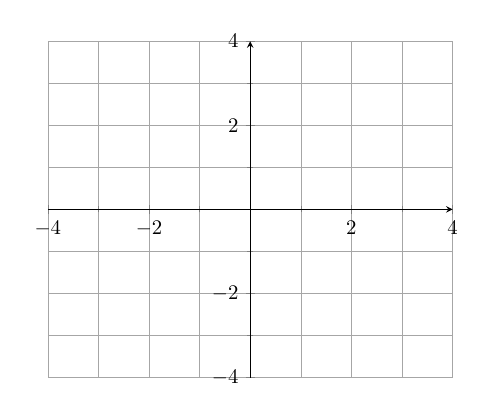
\begin{tikzpicture}[scale=0.75]
      \begin{axis}%
    [grid=both,
     minor tick num=1,
     grid style={line width=.2pt, draw=gray!70},
     major grid style={line width=.2pt,draw=gray!70},
     xtick={-4,-2,...,2,4},
     ytick={-4,-2,...,2,4},
     xmin=-4, xmax=4,
     ymin=-4, ymax=4,
     axis lines=middle,
     enlargelimits=false
    ]
  \end{axis}
\end{tikzpicture}
\end{center}
\fi

\begin{note}
Every function has a graph, but not every graph has a function.
\end{note}

\subsubsection{Vertical Line Test}
\begin{prop}[Vertical line test]
If any vertical line crosses a graph more than once, it does not represent a function.
\end{prop}
\begin{center}
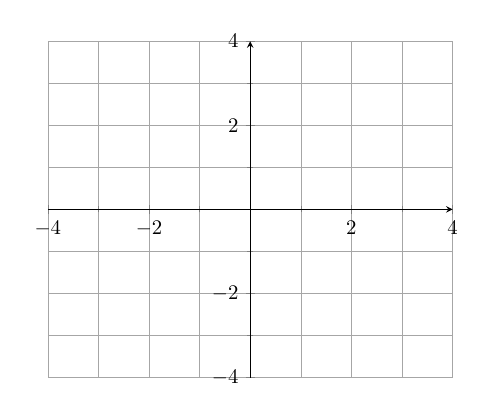
\begin{tikzpicture}[scale=0.75]
      \begin{axis}%
    [grid=both,
     minor tick num=1,
     grid style={line width=.2pt, draw=gray!70},
     major grid style={line width=.2pt,draw=gray!70},
     xtick={-4,-2,...,2,4},
     ytick={-4,-2,...,2,4},
     xmin=-4, xmax=4,
     ymin=-4, ymax=4,
     axis lines=middle,
     enlargelimits=false
    ]
  \end{axis}
\end{tikzpicture}
\hspace{1in}
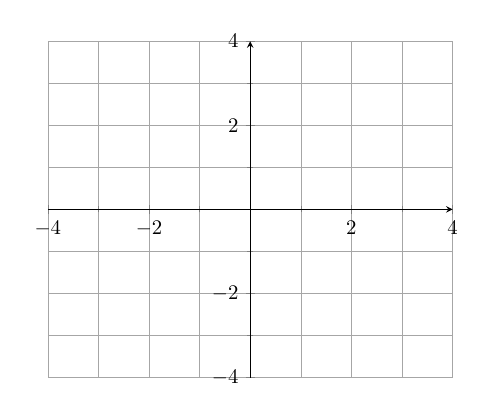
\begin{tikzpicture}[scale=0.75]
      \begin{axis}%
    [grid=both,
     minor tick num=1,
     grid style={line width=.2pt, draw=gray!70},
     major grid style={line width=.2pt,draw=gray!70},
     xtick={-4,-2,...,2,4},
     ytick={-4,-2,...,2,4},
     xmin=-4, xmax=4,
     ymin=-4, ymax=4,
     axis lines=middle,
     enlargelimits=false
    ]
  \end{axis}
\end{tikzpicture}
\end{center}

Here are some other symbols to be familiar with:
\begin{itemize}
    \item \blank{open dot}{open dot} - ends at that point, but does
    NOT include it.
    \item \blank{closed dot}{closed dot} - ends at that point AND includes it.
    \item \blank{arrow}{arrow} - the graph continues in that direction forever.
\end{itemize}

\subsection{Finding Domain and Range from a Graph}

\begin{exercise}
Find the domain and range of the following:
\begin{center}
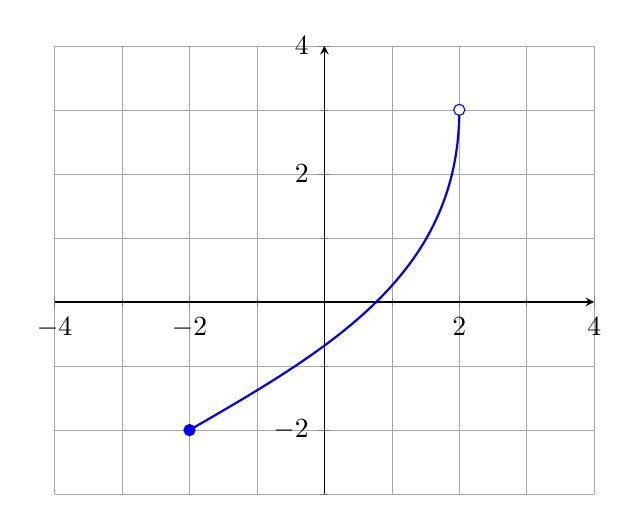
\begin{tikzpicture}
     \begin{axis}%
    [grid=both,
    ymin=-3, ymax=4,
    xmin=-4, xmax=4,
     minor tick num=1,
     grid style={line width=.2pt, draw=gray!70},
     major grid style={line width=.2pt,draw=gray!70},
     axis lines=middle,
     enlargelimits=false
    ]
    \addplot[blue,only marks] coordinates {(-2,-2)};
    \addplot[blue,mark=*,fill=white] coordinates {(2,3)};
    \addplot[blue,smooth,thick] (-2,-2) to[out=30, in=-90] (2,3);
  \end{axis}
\end{tikzpicture}
\end{center}
\end{exercise}
\begin{solution}[0.75in]

\end{solution}

\begin{exercise}
Find the domain and range of the following:
\begin{center}
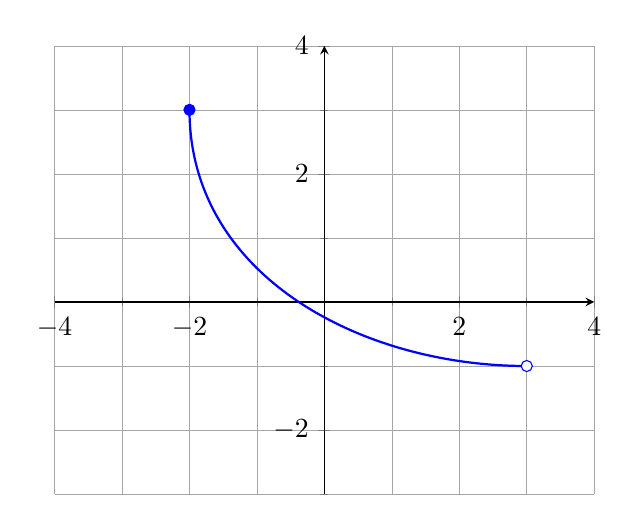
\begin{tikzpicture}
     \begin{axis}%
    [grid=both,
    ymin=-3, ymax=4,
    xmin=-4, xmax=4,
     minor tick num=1,
     grid style={line width=.2pt, draw=gray!70},
     major grid style={line width=.2pt,draw=gray!70},
     axis lines=middle,
     enlargelimits=false
    ]
    \addplot[blue,only marks] coordinates {(-2,3)};
    \addplot[blue,mark=*,fill=white] coordinates {(3,-1)};
    \addplot[blue,smooth,thick] (-2,3) to[out=-90, in=180] (3,-1);
  \end{axis}
\end{tikzpicture}
\end{center}
\end{exercise}
\begin{solution}[=0.75in]

\end{solution}

\begin{exercise}
Find the domain and range of the following:
\begin{center}
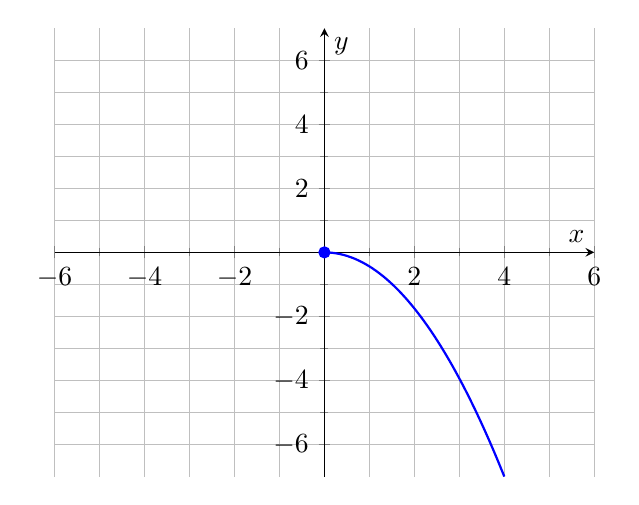
\begin{tikzpicture}
     \begin{axis}%
    [grid=both,
    minor tick num=1,
    axis x line=middle, axis y line=middle,
    ymin=-7, ymax=7, ytick={-6,-4,...,4,6}, ylabel=$y$,
    xmin=-6, xmax=6, xtick={-6,-4,...,4,6}, xlabel=$x$
    ]
    \addplot[blue,mark=*] coordinates {(0,0)};
    \addplot+[blue,smooth,thick,domain=0:4,mark=none] {-7/16*x^2};
  \end{axis}
\end{tikzpicture}
\end{center}
\end{exercise}
\begin{solution}[1in]

\end{solution}
\vspace{0.5em}

\begin{exercise}
Find the domain and range of the function shown below:
\begin{center}
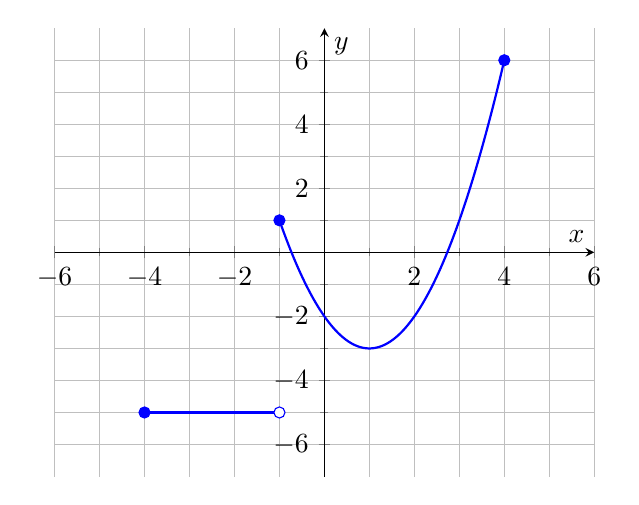
\begin{tikzpicture}
     \begin{axis}%
    [grid=both,
    minor tick num=1,
    axis x line=middle, axis y line=middle,
    ymin=-7, ymax=7, ytick={-6,-4,...,4,6}, ylabel=$y$,
    xmin=-6, xmax=6, xtick={-6,-4,...,4,6}, xlabel=$x$
    ]
    \addplot+[blue,mark=none,thick,domain=-1:4,
     samples=100,] {x^2-2*x-2};
    \addplot[blue,mark=none,thick] (-4,-5)--(-1,-5);
    \addplot[blue,mark=*,only marks] coordinates {(-4,-5) (-1,1) (4,6)};
    \addplot[blue,mark=*,fill=white,only marks] coordinates {(-1,-5)};
  \end{axis}
\end{tikzpicture}
\end{center}
\end{exercise}
\begin{solution}[2in]

\end{solution}
\vspace{0.5em}

\subsection{Finding domains from equations}

For some of these questions instead of asking what numbers work, the easier
question is what numbers ``don't work''.

\begin{exercise}
Find the domain of
\[
f(x)=\frac{1}{(x+3)(x-2)}
\]
\end{exercise}
\begin{solution}[2in]

\end{solution}
\vspace{0.5em}

\begin{exercise}
Find the domain of
\[
g(x)=\sqrt{x+2}
\]
\end{exercise}
\begin{solution}[1.5in]

\end{solution}
\vspace{0.5em}

\begin{exercise}
Find the domain of
\[
q(x)=\frac{1}{\sqrt{8-9x}}
\]
\end{exercise}
\begin{solution}[2in]

\end{solution}
\vspace{0.5em}

\section{Linear Functions}

\subsection{Slope}

\begin{definition}
The \emph{slope} of a line is the following ratio
\[
m=\frac{\emptyfrac{\text{rise}}}{\emptyfrac{\text{run}}}=\frac{\emptyfrac{\text{Change in }y}}{\emptyfrac{\text{Change in }x}}
\]
If $(x_1,y_1)$ \& $(x_2,y_2)$ are two points on a line, then the slope is
\[
m=\frac{\emptyfrac{y_2-y_1}}{\emptyfrac{x_2-x_1}}
\]
\end{definition}
\vspace{0.5em}

\begin{exercise}
Find the slope of the line between $(-3,4)$ \& $(-4,-2)$.
\end{exercise}
\begin{solution}[1in]

\end{solution}
\vspace{0.5em}

\begin{exercise}
Find the slope of the line between $(4,-2)$ \& $(-1,5)$.
\end{exercise}
\begin{solution}[1in]

\end{solution}
\vspace{0.5em}

\begin{exercise}
Find the slope of the line between $(7,-3)$ \& $(1,11)$.
\end{exercise}
\begin{solution}[1in]

\end{solution}
\vspace{0.5em}

\subsection{Graphs}

\vspace{3em}

\ifprintanswers
\else
\begin{center}
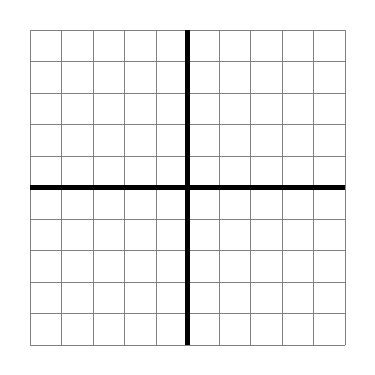
\begin{tikzpicture}[scale=0.4]
\draw[step=1cm,gray,very thin] (-5,-5) grid (5,5);
\draw[black,ultra thick] (-5,0) -- (5,0);
\draw[black,ultra thick] (0,-5) -- (0,5);
\end{tikzpicture}
\hspace{2in}
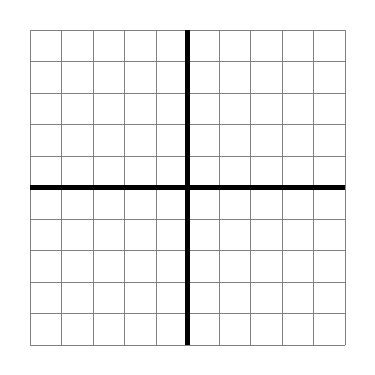
\begin{tikzpicture}[scale=0.4]
\draw[step=1cm,gray,very thin] (-5,-5) grid (5,5);
\draw[black,ultra thick] (-5,0) -- (5,0);
\draw[black,ultra thick] (0,-5) -- (0,5);
\end{tikzpicture}

\vspace{5em}

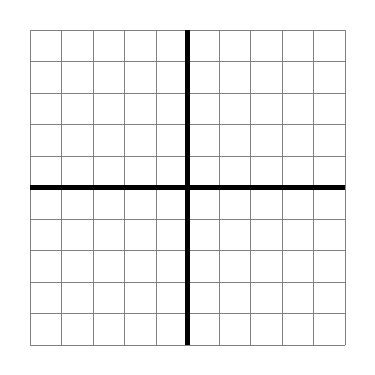
\begin{tikzpicture}[scale=0.4]
\draw[step=1cm,gray,very thin] (-5,-5) grid (5,5);
\draw[black,ultra thick] (-5,0) -- (5,0);
\draw[black,ultra thick] (0,-5) -- (0,5);
\end{tikzpicture}
\hspace{2in}
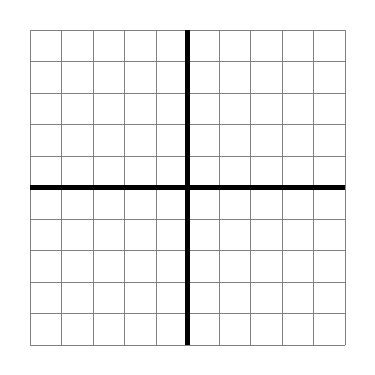
\begin{tikzpicture}[scale=0.4]
\draw[step=1cm,gray,very thin] (-5,-5) grid (5,5);
\draw[black,ultra thick] (-5,0) -- (5,0);
\draw[black,ultra thick] (0,-5) -- (0,5);
\end{tikzpicture}
\end{center}
\fi

\subsubsection{Slope-Intercept form}

\vspace{0.5em}

\begin{center}
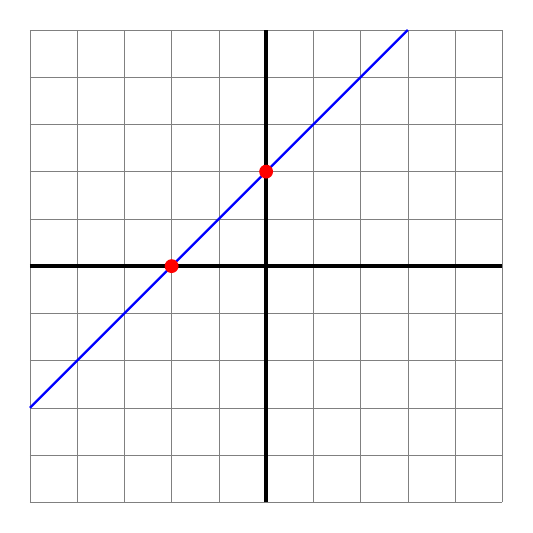
\begin{tikzpicture}[scale=0.6]
\draw[step=1cm,gray,very thin] (-5,-5) grid (5,5);
\draw[black,ultra thick] (-5,0) -- (5,0);
\draw[black,ultra thick] (0,-5) -- (0,5);

\draw[blue,thick] (-5,-3) -- (3,5);
\node[circle,fill=red,inner sep=0pt,minimum size=5pt](x) at (-2,0) {};
\node[circle,fill=red,inner sep=0pt,minimum size=5pt](y) at (0,2) {};
\end{tikzpicture}   
\end{center}

\vspace{0.5em}

\begin{definition}[Slope-intercept form]\label{def: slope-intercept form}
A line with slope $m$ and $y$-intercept $b$ has the equation
\[
y=\blank{mx+b}{mx+b}
\]
\end{definition}

\vspace{0.5em}

\begin{exercise}
What are the slope and $y$-intercept of $y=3x-4$?
\end{exercise}
\begin{solution}[1in]

\end{solution}

\begin{exercise}
What is the $x$ intercept of $f(x)=2x-8$?
\end{exercise}
\begin{solution}[1in]

\end{solution}

\begin{exercise}
Find the slope-intercept form of the line with slope $7$ and $y$-intercept $2$.
\end{exercise}
\begin{solution}[1in]

\end{solution}

\subsection{Graphing Lines}
\begin{exercise}
Graph $f(x)=2x+5$
\end{exercise}
\ifprintanswers
\else
\begin{center}
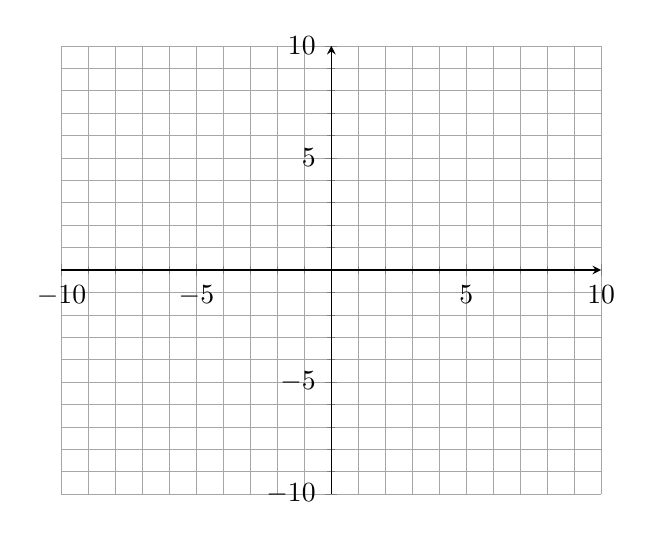
\begin{tikzpicture}
      \begin{axis}%
    [grid=both,
     minor tick num=4,
     grid style={line width=.2pt, draw=gray!70},
     major grid style={line width=.2pt,draw=gray!70},
     xtick={-10,-5,...,5,10},
     ytick={-10,-5,...,5,10},
     xmin=-10, xmax=10,
     ymin=-10, ymax=10,
     axis lines=middle,
     enlargelimits=false
    ]
  \end{axis}
\end{tikzpicture}       
\end{center}
\fi

\newpage

\begin{exercise}
Graph $h(x)=-3x-6$
\end{exercise}
\ifprintanswers
\else
\begin{center}
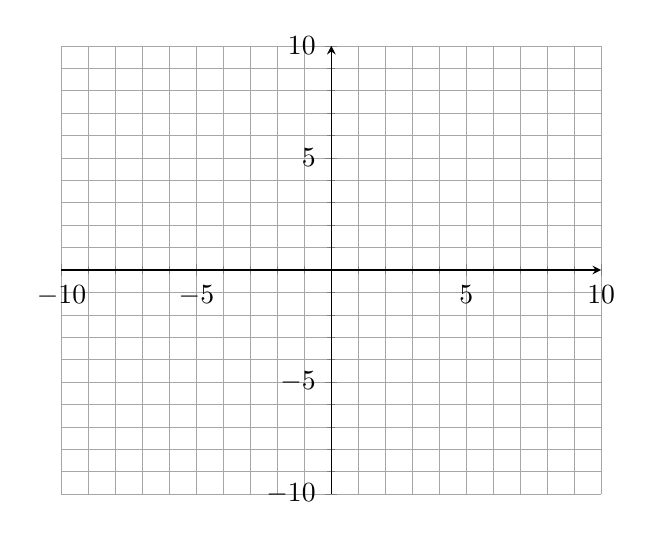
\begin{tikzpicture}
      \begin{axis}%
    [grid=both,
     minor tick num=4,
     grid style={line width=.2pt, draw=gray!70},
     major grid style={line width=.2pt,draw=gray!70},
     xtick={-10,-5,...,5,10},
     ytick={-10,-5,...,5,10},
     xmin=-10, xmax=10,
     ymin=-10, ymax=10,
     axis lines=middle,
     enlargelimits=false
    ]
  \end{axis}
\end{tikzpicture} 
\end{center}
\fi

\begin{exercise}
Find $y=mx+b$ for the following:
\begin{center}
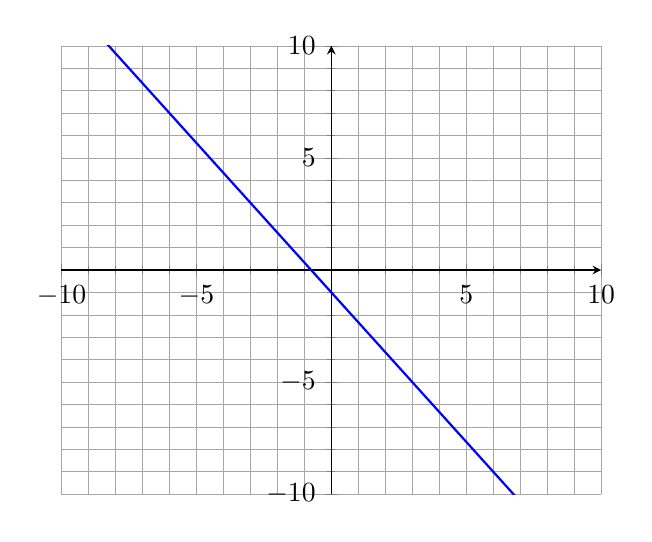
\begin{tikzpicture}
      \begin{axis}%
    [grid=both,
     minor tick num=4,
     grid style={line width=.2pt, draw=gray!70},
     major grid style={line width=.2pt,draw=gray!70},
     xtick={-10,-5,...,5,10},
     ytick={-10,-5,...,5,10},
     xmin=-10, xmax=10,
     ymin=-10, ymax=10,
     axis lines=middle,
     enlargelimits=false
    ]
      \addplot[blue,thick,domain=-10:10] {-4/3*x-1};
  \end{axis}
\end{tikzpicture}
\end{center}
\end{exercise}

\section{More on Lines}

\subsection{Finding the equation of a line}

In general, to find the equation of a line we need the slope and any point on the line.

\vspace{0.5em}

\begin{definition}[Point-slope form]\label{def: point slope form}
If we have a point $(x_1,y_1)$ on a line with slope $m$, then the \emph{point-slope form} is
\[
\blank{y-y_1}{y-y_1}=\blank{m(x-x_1)}{m(x-x_1)}
\]
\end{definition}

\newpage

\begin{exercise}
Find the equation of a line passing through $(2,-5)$ with slope $m=6$ in slope-intercept form.
\end{exercise}
\begin{solution}[3in]

\end{solution}

\begin{exercise}
Find the equation of a line passing through $(3,4)$ with slope $m=-5$ in slope-intercept form.
\end{exercise}
\begin{solution}[2in]

\end{solution}

\begin{exercise}
Find the equation of a line passing through $(3,4)$ \& $(-1,-6)$ in slope-intercept form.
\end{exercise}
\begin{solution}[2in]

\end{solution}

\subsection{Standard Form}

\begin{definition}[Standard form]\label{def: standard from of a line}
If $A$, $B$, and $C$ are integers (with $A>0$), then the standard form of a line is
\[
\blank{Ax+By}{Ax+By}=\blank{C}{C}\quad\text{or}\quad\blank{Ax+By+C}{Ax+By+C}=\blank{0}{0}
\]
\end{definition}

\begin{exercise}
Find the standard form of the line passing through $(-8,-1)$ \& $(-1,-2)$.
\end{exercise}
\begin{solution}[2in]

\end{solution}

\begin{exercise}
Find the standard form of the line passing through $(-7,-4)$ \& $(-2,3)$.
\end{exercise}
\begin{solution}[2in]

\end{solution}

\subsection{Horizontal \& Vertical Lines}

\begin{note}
A horizontal line has a slope of \blank{0}{0}. This means that their equation
is
\[
y=\blank{0x+b}{0x+b}=\blank{0+b}{0+b}=\blank{b}{b}
\]
Every horizontal line can be written this way, which makes sense because the
\blank{$y$-value}{$y$-value} never changes.
\end{note}

\vspace{0.5em}

\begin{note}
In a similar way, the \blank{$x$-value}{$x$-value} never changes for vertical lines,
their equation looks like
\[
\blank{x}{x}=\blank{a}{a}
\]
\end{note}

\vspace{0.5em}

\begin{exercise}
What is the equation of the following line?
\begin{center}
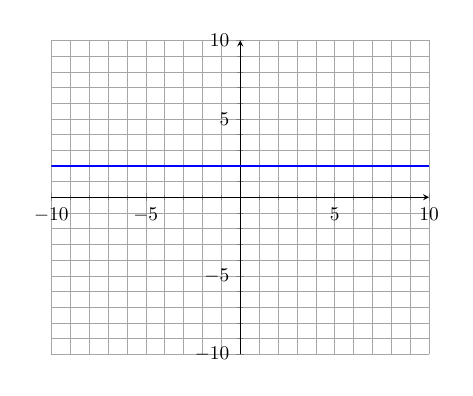
\begin{tikzpicture}[scale=.7]
      \begin{axis}%
    [grid=both,
     minor tick num=4,
     grid style={line width=.2pt, draw=gray!70},
     major grid style={line width=.2pt,draw=gray!70},
     xtick={-10,-5,...,5,10},
     ytick={-10,-5,...,5,10},
     xmin=-10, xmax=10,
     ymin=-10, ymax=10,
     axis lines=middle,
     enlargelimits=false
    ]
      \addplot[blue,thick,domain=-10:10] {2};
  \end{axis}
\end{tikzpicture}  
\end{center}
\end{exercise}

\vspace{0.5em}

\begin{exercise}
What is the equation of the following line?
\begin{center}
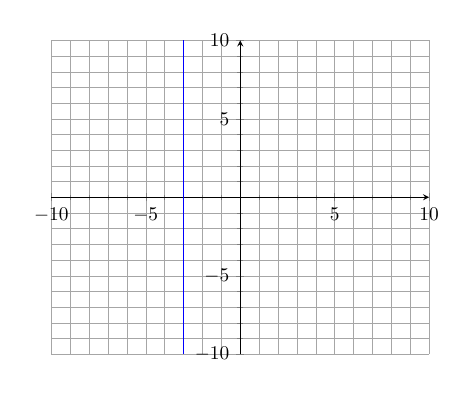
\begin{tikzpicture}[scale=.7]
      \begin{axis}%
    [grid=both,
     minor tick num=4,
     grid style={line width=.2pt, draw=gray!70},
     major grid style={line width=.2pt,draw=gray!70},
     xtick={-10,-5,...,5,10},
     ytick={-10,-5,...,5,10},
     xmin=-10, xmax=10,
     ymin=-10, ymax=10,
     axis lines=middle,
     enlargelimits=false
    ]
     \draw[blue,thick] (-3,-10) -- (-3,10);
  \end{axis}
\end{tikzpicture}
\end{center}
\end{exercise}

\subsection{Parallel and Perpendicular Lines}

\begin{definition}\label{def: Parallel lines}
Two lines are called \emph{parallel} (denoted by $\parallel$) 
if they \blank{never intersect}{never intersect}
\end{definition}

\begin{prop}\label{prop: parallel line conditions}
\text{}
\begin{itemize}
    \item Two distinct non-vertical lines are parallel if and only if
   \blank{they have the same slope}{they have the same slope}.
   \item If two vertical lines are \blank{distinct}{distinct}, then
   they are parallel.
\end{itemize}
\end{prop}

\begin{exercise}
Find the slope-intercept form of a line passing through $(-2,5)$
and parallel to $y=3x+1$.
\end{exercise}
\begin{solution}[2in]

\end{solution}

\newpage

\begin{exercise}
Find the line parallel to $y=5x-9$ passing through $(4,-2)$ in slope-intercept form.
\end{exercise}
\begin{solution}[2in]

\end{solution}

\begin{definition}
Two lines are called \emph{perpendicular} (denoted by $\perp$) if they
\blank{intersect at a $90^\circ$}{intersect at a $90^\circ$}.
\end{definition}

\begin{prop}\label{prop: perp line conditions}
\text{}
\begin{itemize}
    \item Two distinct non-vertical lines are perpendicular if and only if the
    product of their slopes is \blank{$-1$}{$-1$}.
   \item Horizontal and vertical lines are \blank{always}{always} perpendicular.
\end{itemize}
\end{prop}

\begin{note}
Another way to understand the first point is if the one slope is $m=\frac{a}{b}$,
then the perpendicular slope is $m_\perp=\blank{-\frac{b}{a}}{-\frac{b}{a}}$
\end{note}

\begin{exercise}
Find a line through $(-2,-6)$ and perpendicular to $y=-\frac{1}{3}x+4$ in slope-intercept form.
\end{exercise}
\begin{solution}[2in]

\end{solution}

\newpage

\begin{exercise}
Find the equation of the line perpendicular to $y=\frac{1}{4}x-4$
and passing through $(-8,5)$ in slope-intercept form.
\end{exercise}
\begin{solution}[2in]

\end{solution}

\vspace{0.5em}

\begin{exercise}
Are the following two lines parallel, perpendicular, or neither?
\[
y=3x-5\quad y+\frac{1}{3}x=2
\]
\end{exercise}
\begin{solution}[1.5in]

\end{solution}

\subsection{Real-World Applications}

\begin{exercise}
You are considering using a moving company to help you move. They charge \$60 per hour
plus a base fee of \$290. If $C$ is the total cost of hiring the moving company and $H$
is the number of hours worked, what is the relationship between $H$ and $C$?
\end{exercise}
\begin{solution}[3in]

\end{solution}

\section{Transformations of Graphs/Functions}

\subsection{The Basic Transformations}

Let $f(x)$ be a function. Then there are 4 (or 6) basic transformations:

\begin{enumerate}[1)]
\item Vertical Shifts
\[
\blank{f(x)\pm c}{f(x)\pm c}
\]
\vspace{1.5em}

\item Horizontal Shifts
\[
\blank{f(x\pm c)}{f(x\pm c)}
\]
\vspace{3em}

\item Vertical stretches \& shrinks/compressions
\[
\blank{cf(x)}{cf(x)}
\]
\vspace{3em}

\begin{enumerate}[3.5)]
\item Vertical ($x$-axis) Reflection
\[
\blank{-1f(x)}{-1f(x)}
\]
\end{enumerate}

\vspace{3em}

\item Horizontal stretches \& shrinks/compressions
\[
\blank{f(c x)}{f(c x)}
\]
\vspace{3em}
\begin{enumerate}[4.5)]
\item Horizontal ($y$-axis) Reflection
\[
\blank{f(-1x)}{f(-1x)}
\]
\vspace{3em}
\end{enumerate}
\end{enumerate}

\newpage

\begin{example}
Vertical shift: Transform $f(x)$ to $f(x)+2$
\end{example}
\ifprintanswers
\else
\begin{center}
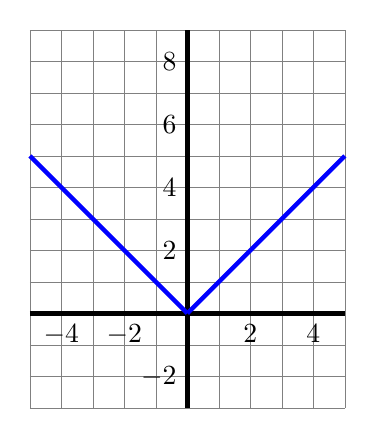
\begin{tikzpicture}[scale=0.4]
\draw[step=1cm,gray,very thin] (-5,-3) grid (5,9);
\draw[black,ultra thick] (-5,0) -- (5,0);
\draw[black,ultra thick] (0,-3) -- (0,9);

\foreach\x/\xtext in {-4,-2,2,4}
\draw (\x ,1pt) -- (\x,-1pt) node[anchor=north] {$\xtext$};
\foreach\y/\ytext in {-2,2,4,6,8}
\draw (1pt,\y) -- (-1pt,\y) node[anchor=east] {$\ytext$};
\draw[blue,ultra thick] (-5,5) -- (0,0);
\draw[blue,ultra thick] (5,5) -- (0,0);
\end{tikzpicture}
\end{center}
\fi

\begin{example}
Horizontal shift: Find $f(x+3)$ using $f(x)$ below
\end{example}
\ifprintanswers
\else
\begin{center}
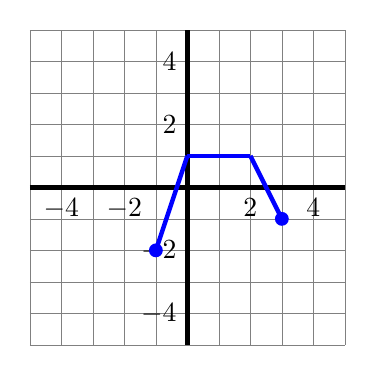
\begin{tikzpicture}[scale=0.4]
\draw[step=1cm,gray,very thin] (-5,-5) grid (5,5);
\draw[black,ultra thick] (-5,0) -- (5,0);
\draw[black,ultra thick] (0,-5) -- (0,5);

\foreach\x/\xtext in {-4,-2,2,4}
\draw (\x ,1pt) -- (\x,-1pt) node[anchor=north] {$\xtext$};
\foreach\y/\ytext in {-4,-2,2,4}
\draw (1pt,\y) -- (-1pt,\y) node[anchor=east] {$\ytext$};
\draw[blue,ultra thick] (-1,-2) -- (0,1);
\draw[blue,ultra thick] (0,1) -- (2,1);
\draw[blue,ultra thick] (2,1) -- (3,-1);
\node[circle,fill=blue,inner sep=0pt,minimum size=5pt](x) at (-1,-2) {};
\node[circle,fill=blue,inner sep=0pt,minimum size=5pt](y) at (3,-1) {};
\end{tikzpicture}
\end{center}
\fi

\begin{example}
Vertical Stretch \& Shrink/Compression: Find $3f(x)$ using $f(x)$ below
\end{example}
\ifprintanswers
\else
\begin{center}
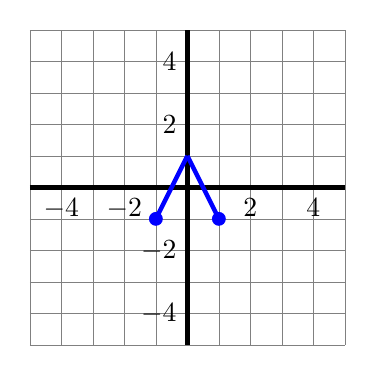
\begin{tikzpicture}[scale=0.4]
\draw[step=1cm,gray,very thin] (-5,-5) grid (5,5);
\draw[black,ultra thick] (-5,0) -- (5,0);
\draw[black,ultra thick] (0,-5) -- (0,5);

\foreach\x/\xtext in {-4,-2,2,4}
\draw (\x ,1pt) -- (\x,-1pt) node[anchor=north] {$\xtext$};
\foreach\y/\ytext in {-4,-2,2,4}
\draw (1pt,\y) -- (-1pt,\y) node[anchor=east] {$\ytext$};
\draw[blue,ultra thick] (-1,-1) -- (0,1);
\draw[blue,ultra thick] (0,1) -- (1,-1);
\node[circle,fill=blue,inner sep=0pt,minimum size=5pt](x) at (-1,-1) {};
\node[circle,fill=blue,inner sep=0pt,minimum size=5pt](y) at (1,-1) {};
\end{tikzpicture}
\end{center}
\fi

\begin{example}
Horizontal Stretch \& Shrink/Compression:
Find $f(-2x)$ using $f(x)$ below
\end{example}
\ifprintanswers
\else
\begin{center}
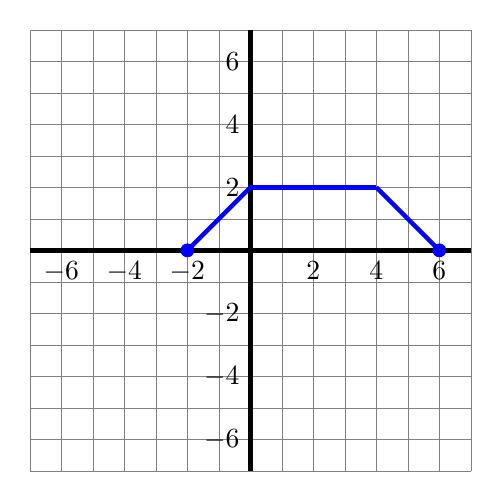
\begin{tikzpicture}[scale=0.4]
\draw[step=1cm,gray,very thin] (-7,-7) grid (7,7);
\draw[black,ultra thick] (-7,0) -- (7,0);
\draw[black,ultra thick] (0,-7) -- (0,7);

\foreach\x/\xtext in {-6,-4,-2,2,4,6}
\draw (\x ,1pt) -- (\x,-1pt) node[anchor=north] {$\xtext$};
\foreach\y/\ytext in {-6,-4,-2,2,4,6}
\draw (1pt,\y) -- (-1pt,\y) node[anchor=east] {$\ytext$};
\draw[blue,ultra thick] (-2,0) -- (0,2);
\draw[blue,ultra thick] (0,2) -- (4,2);
\draw[blue,ultra thick] (4,2) -- (6,0);
\node[circle,fill=blue,inner sep=0pt,minimum size=5pt](x) at (-2,-0) {};
\node[circle,fill=blue,inner sep=0pt,minimum size=5pt](y) at (6,0) {};
\end{tikzpicture}
\end{center}
\fi

\subsection{Describing transformations}

\begin{exercise}
Describe the graph of $y=3f(x-2)+4$ in terms of the graph
of $y=f(x)$.
\end{exercise}
\begin{solution}[1in]

\end{solution}

\begin{exercise}
Describe the graph of $y=\frac{1}{4}f(-x+2)$ in terms of the graph
of $y=f(x)$.
\end{exercise}
\begin{solution}[1in]

\end{solution}

\subsection{Graphing multiple transformations}

\begin{note}
Here is a rule of thumb for transformations:
\begin{itemize}
    \item Work inside to outside.
    \item Multiplication/division before addition/subtraction
\end{itemize}
\end{note}

\begin{exercise}
Graph $y=f(-x+3)-4$ using the graph of $y=f(x)$ below:
\end{exercise}
\ifprintanswers
\else
\begin{center}
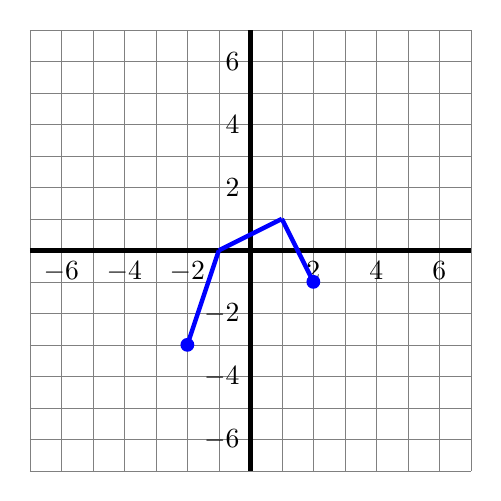
\begin{tikzpicture}[scale=0.4]
\draw[step=1cm,gray,very thin] (-7,-7) grid (7,7);
\draw[black,ultra thick] (-7,0) -- (7,0);
\draw[black,ultra thick] (0,-7) -- (0,7);

\foreach\x/\xtext in {-6,-4,-2,2,4,6}
\draw (\x ,1pt) -- (\x,-1pt) node[anchor=north] {$\xtext$};
\foreach\y/\ytext in {-6,-4,-2,2,4,6}
\draw (1pt,\y) -- (-1pt,\y) node[anchor=east] {$\ytext$};
\draw[blue,ultra thick] (-2,-3) -- (-1,0);
\draw[blue,ultra thick] (-1,0) -- (1,1);
\draw[blue,ultra thick] (1,1) -- (2,-1);
\node[circle,fill=blue,inner sep=0pt,minimum size=5pt](x) at (-2,-3) {};
\node[circle,fill=blue,inner sep=0pt,minimum size=5pt](y) at (2,-1) {};
\end{tikzpicture}
\end{center}
\fi
\begin{solution}[1in]

\end{solution}

\newpage

\begin{exercise}
Graph $y=3f(x+2)-1$ using the graph of $y=f(x)$ below:
\end{exercise}
\ifprintanswers
\else
\begin{center}
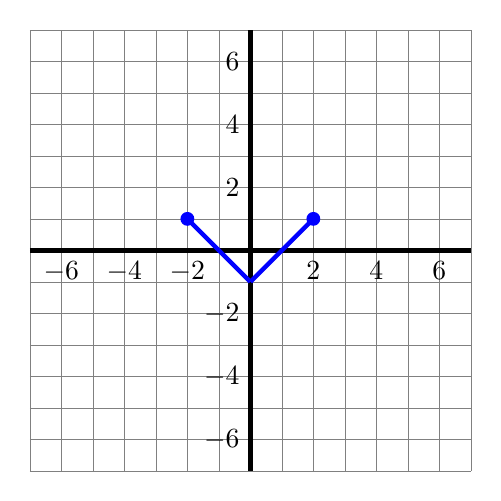
\begin{tikzpicture}[scale=0.4]
\draw[step=1cm,gray,very thin] (-7,-7) grid (7,7);
\draw[black,ultra thick] (-7,0) -- (7,0);
\draw[black,ultra thick] (0,-7) -- (0,7);

\foreach\x/\xtext in {-6,-4,-2,2,4,6}
\draw (\x ,1pt) -- (\x,-1pt) node[anchor=north] {$\xtext$};
\foreach\y/\ytext in {-6,-4,-2,2,4,6}
\draw (1pt,\y) -- (-1pt,\y) node[anchor=east] {$\ytext$};
\draw[blue,ultra thick] (-2,1) -- (0,-1);
\draw[blue,ultra thick] (0,-1) -- (2,1);
\node[circle,fill=blue,inner sep=0pt,minimum size=5pt](x) at (-2,1) {};
\node[circle,fill=blue,inner sep=0pt,minimum size=5pt](y) at (2,1) {};
\end{tikzpicture}
\end{center}
\fi
\begin{solution}[1in]

\end{solution}

\begin{exercise}
Graph $y=3f(2x-2)+2$ using the graph of $y=f(x)$ below:
\end{exercise}
\ifprintanswers
\else
\begin{center}
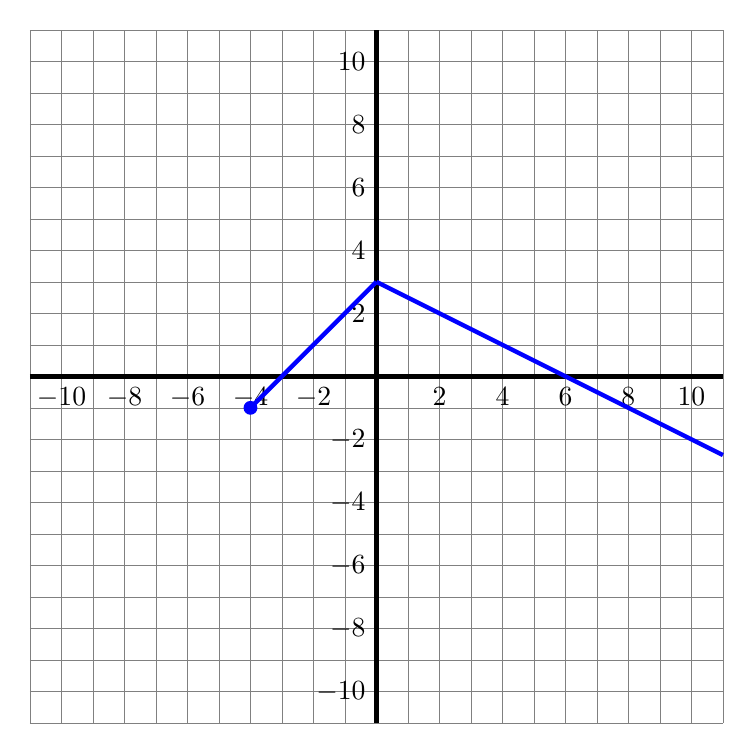
\begin{tikzpicture}[scale=0.4]
\draw[step=1cm,gray,very thin] (-11,-11) grid (11,11);
\draw[black,ultra thick] (-11,0) -- (11,0);
\draw[black,ultra thick] (0,-11) -- (0,11);

\foreach\x/\xtext in {-10,-8,-6,-4,-2,2,4,6,8,10}
\draw (\x ,1pt) -- (\x,-1pt) node[anchor=north] {$\xtext$};
\foreach\y/\ytext in {-10,-8,-6,-4,-2,2,4,6,8,10}
\draw (1pt,\y) -- (-1pt,\y) node[anchor=east] {$\ytext$};
\draw[blue,ultra thick] (-4,-1) -- (0,3);
\draw[blue,ultra thick] (0,3) -- (11,-5/2);
\node[circle,fill=blue,inner sep=0pt,minimum size=5pt](x) at (-4,-1) {};
\end{tikzpicture}
\end{center}
\fi
\begin{solution}[1in]

\end{solution}

\newpage

\begin{exercise}
Using $y=f(x)$ below, graph $y=f(-x-3)+1$
\end{exercise}
\ifprintanswers
\else
\begin{center}
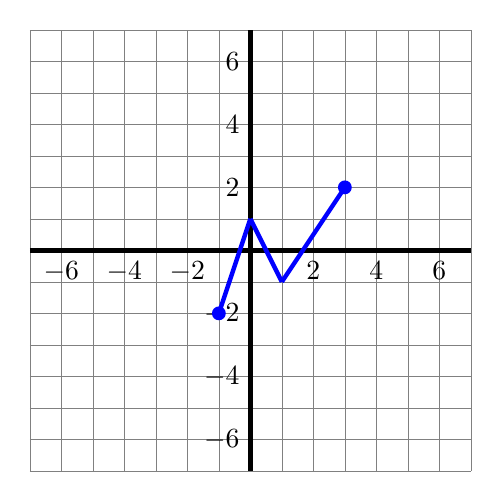
\begin{tikzpicture}[scale=0.4]
\draw[step=1cm,gray,very thin] (-7,-7) grid (7,7);
\draw[black,ultra thick] (-7,0) -- (7,0);
\draw[black,ultra thick] (0,-7) -- (0,7);

\foreach\x/\xtext in {-6,-4,-2,2,4,6}
\draw (\x ,1pt) -- (\x,-1pt) node[anchor=north] {$\xtext$};
\foreach\y/\ytext in {-6,-4,-2,2,4,6}
\draw (1pt,\y) -- (-1pt,\y) node[anchor=east] {$\ytext$};
\draw[blue,ultra thick] (-1,-2) -- (0,1);
\draw[blue,ultra thick] (0,1) -- (1,-1);
\draw[blue,ultra thick] (1,-1) -- (3,2);
\node[circle,fill=blue,inner sep=0pt,minimum size=5pt](x) at (-1,-2) {};
\node[circle,fill=blue,inner sep=0pt,minimum size=5pt](x) at (3,2) {};
\end{tikzpicture}
\end{center}
\fi
\begin{solution}[1in]

\end{solution}


\section{More on Functions \& Piece-wise Functions}

\subsection{Even and Odd Functions}

There are two ways to see whether a functions is even, odd or neither.

\subsubsection*{Algebraically}
\begin{definition}\label{def: even and odd functions}
\text{}
\begin{itemize}
    \item If $f(x)$ is odd, then $f(-x)=\blank{-f(x)}{-f(x)}$.
    \item If $f(x)$ is even, then $f(-x)=\blank{f(x)}{f(x)}$.
\end{itemize}
\end{definition}

\begin{exercise}
Is $f(x)=x^2+6$ even, odd, or neither?
\end{exercise}
\begin{solution}[2in]

\end{solution}
\vspace{0.5em}

\begin{exercise}
Is $g(x)=x^3-x$ even, odd, or neither?
\end{exercise}
\begin{solution}[2in]

\end{solution}
\vspace{0.5em}

\begin{exercise}
Is $h(x)=x^5+1$ even, odd, or neither?
\end{exercise}
\begin{solution}[2in]

\end{solution}
\vspace{0.5em}

Notice the following
\begin{itemize}
    \item $f(x)$ had all even powers.
    \item $g(x)$ had all odd powers.
    \item $h(x)$ had both even and odd powers.
\end{itemize}

\begin{fact}
\text{}
\begin{itemize}
    \item If all the powers in a polynomial are \blank{even}{even}, then it is as an even function.
    \item If all the powers in a polynomial are \blank{odd}{odd}, then it is as an odd function.
\end{itemize}
\end{fact}

\newpage

\subsubsection*{Graphically}

Recall that if $f(x)$ is even, then $f(-x)=f(x)$. This means that $x$
and $-x$ have the same value. So $f(x)$ is even if it has
\blank{$y$-axis symmetry}{$y$-axis symmetry}

\ifprintanswers
\else
\begin{center}
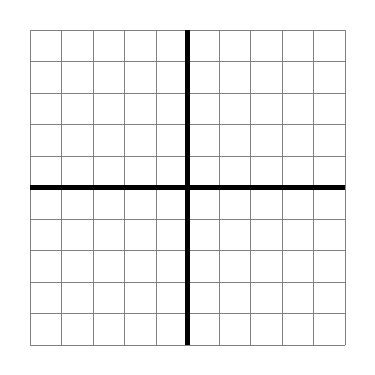
\begin{tikzpicture}[scale=0.4]
\draw[step=1cm,gray,very thin] (-5,-5) grid (5,5);
\draw[black,ultra thick] (-5,0) -- (5,0);
\draw[black,ultra thick] (0,-5) -- (0,5);
\end{tikzpicture}
\hspace{2in}
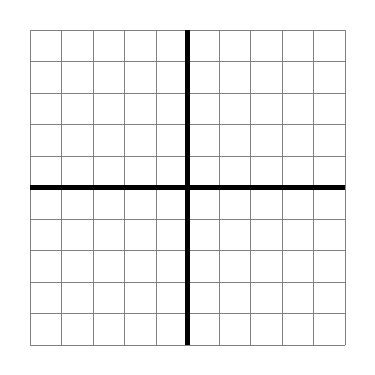
\begin{tikzpicture}[scale=0.4]
\draw[step=1cm,gray,very thin] (-5,-5) grid (5,5);
\draw[black,ultra thick] (-5,0) -- (5,0);
\draw[black,ultra thick] (0,-5) -- (0,5);
\end{tikzpicture}
\end{center}
\fi

If $f(x)$ is instead odd, then $f(-x)=-f(x)$. This means that $x$
and $-x$ have opposite values, so we say that $f(x)$ is odd if it
has \blank{origin symmetry}{symmetry}.

\ifprintanswers
\else
\begin{center}
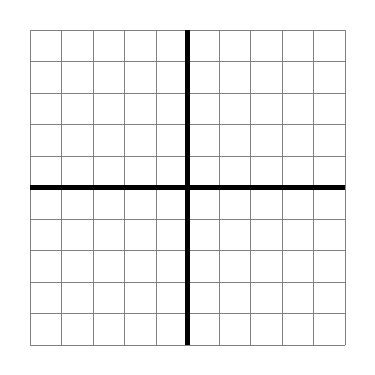
\begin{tikzpicture}[scale=0.4]
\draw[step=1cm,gray,very thin] (-5,-5) grid (5,5);
\draw[black,ultra thick] (-5,0) -- (5,0);
\draw[black,ultra thick] (0,-5) -- (0,5);
\end{tikzpicture}
\hspace{2in}
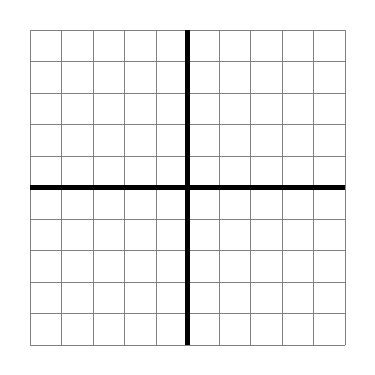
\begin{tikzpicture}[scale=0.4]
\draw[step=1cm,gray,very thin] (-5,-5) grid (5,5);
\draw[black,ultra thick] (-5,0) -- (5,0);
\draw[black,ultra thick] (0,-5) -- (0,5);
\end{tikzpicture}
\end{center}
\fi

\subsection{Piece-wise functions}

\begin{definition}\label{def: piecewise function}
A \emph{piece-wise defined function} or \emph{piece-wise} function
is a function that is defined by different functions on different
parts of its domain. Said another way, piece-wise functions are made
of ``pieces'' of other functions.
\end{definition}

\begin{example}
\[
f(x)=
\begin{cases}
2x-1 & \text{if }x<-1\\
x+1 & \text{if }x\geq-1
\end{cases}
\]
\end{example}

\newpage

\subsubsection*{Graphing}

\begin{exercise}
Graph
\[
f(x)=
\begin{cases}
2x-1 & \text{if }x<-1\\
x+1 & \text{if }x\geq-1
\end{cases}
\]
\end{exercise}
\ifprintanswers
\else
\begin{center}
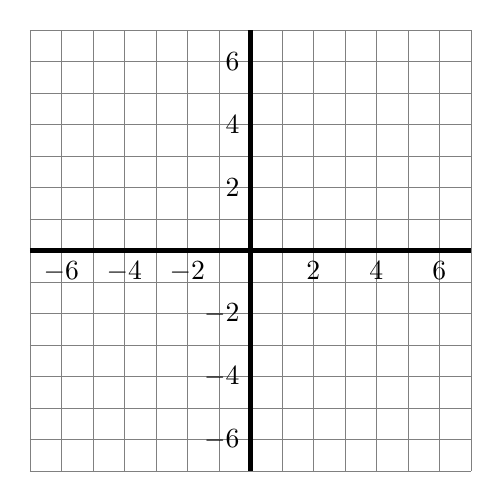
\begin{tikzpicture}[scale=0.4]
\draw[step=1cm,gray,very thin] (-7,-7) grid (7,7);
\draw[black,ultra thick] (-7,0) -- (7,0);
\draw[black,ultra thick] (0,-7) -- (0,7);

\foreach\x/\xtext in {-6,-4,-2,2,4,6}
\draw (\x ,1pt) -- (\x,-1pt) node[anchor=north] {$\xtext$};
\foreach\y/\ytext in {-6,-4,-2,2,4,6}
\draw (1pt,\y) -- (-1pt,\y) node[anchor=east] {$\ytext$};
\end{tikzpicture}
\end{center}
\fi
\begin{solution}[1in]

\end{solution}

\begin{exercise}
Graph
\[
g(x)=
\begin{cases}
\vert x\vert & \text{if }x\leq2\\
1 & \text{if }x>2
\end{cases}
\]
\end{exercise}
\ifprintanswers
\else
\begin{center}
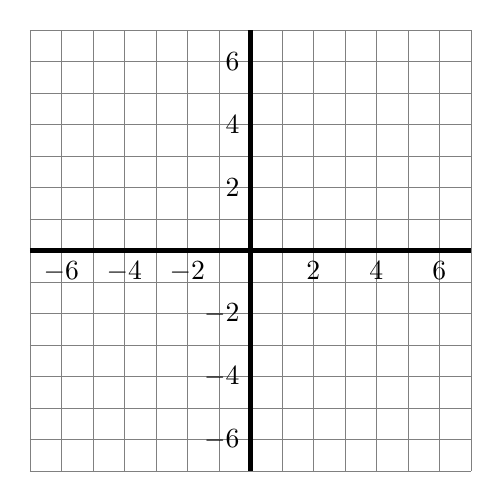
\begin{tikzpicture}[scale=0.4]
\draw[step=1cm,gray,very thin] (-7,-7) grid (7,7);
\draw[black,ultra thick] (-7,0) -- (7,0);
\draw[black,ultra thick] (0,-7) -- (0,7);

\foreach\x/\xtext in {-6,-4,-2,2,4,6}
\draw (\x ,1pt) -- (\x,-1pt) node[anchor=north] {$\xtext$};
\foreach\y/\ytext in {-6,-4,-2,2,4,6}
\draw (1pt,\y) -- (-1pt,\y) node[anchor=east] {$\ytext$};
\end{tikzpicture}
\end{center}
\fi
\begin{solution}[1in]

\end{solution}

\newpage

\subsubsection*{Evaluating}

\begin{exercise}
Find $f(2)$ for
\[
f(x)=
\begin{cases}
-2x & \text{if }x<1\\
x+2 & \text{if }1\leq x<3\\
x^2+2 & \text{if }3\leq x
\end{cases}
\]
\end{exercise}
\begin{solution}[2in]

\end{solution}

\vspace{0.5em}

\begin{exercise}
For
\[
g(x)=
\begin{cases}
-6x+4 & \text{if }x<3\\
3x-5 & \text{if } x\geq3
\end{cases}
\]
find $g(3)$.
\end{exercise}
\begin{solution}[2in]

\end{solution}

\ifprintanswers\else\newpage\fi

\section{Algebra of Functions}

\subsection{Basics}

Let $f(x)$ \& $g(x)$ be two functions and $D_f$ \& $D_g$ be their
domains

\begin{center}
\begin{tabular}{r|c}
Functions & Domains\\\hline
& \\
Sum: $(f+g)(x)=\blank{f(x)+g(x)}{f(x)+g(x)}$ & $\blank{D_f\cap D_g}{D_f \cap D_g}$\\
& \\
Difference: $(f-g)(x)=\blank{f(x)-g(x)}{f(x)-g(x)}$ & $\blank{D_f\cap D_g}{D_f\cap D_g}$\\
& \\
Product: $(fg)(x)=\blank{f(x)\cdot g(x)}{f(x)\cdot g(x)}$ & $\blank{D_f\cap D_g}{D_f\cap D_g}$\\
& \\
Quotient: $\dl\left(\frac{f}{g}\right)(x)=\blank{\frac{f(x)}{g(x)}}{\frac{f(x)}{g(x)}}$ & $\blank{D_f\cap D_g\setminus\{x\mid g(x)=0\}}{D_f\cap D_g\setminus\{x\mid g(x)=0\}}$
\end{tabular}
\end{center}

\begin{exercise}
For $f(x)=x^2-1$ \& $g(x)=3x-4$, find:
\end{exercise}
\ifprintanswers
\else
\begin{itemize}
    \item $(f+g)(x)=$
    \item $(f-g)(x)=$
    \item $(fg)(x)=$
    \item $\dl\left(\frac{f}{g}\right)(x)=$
\end{itemize}
\fi

\subsection{Composite Functions}

\begin{definition}\label{def: composite function}
Given two functions $f(x)$ and $g(x)$, the \emph{composition of $f$ and $g$} ($f$ compose $g$) is the following:
\[
(f\circ g)(x)=\blank{f(g(x))}{f(g(x))}
\]
\end{definition}
\vspace{0.5em}

\begin{exercise}
For $f(x)=4x+3$ and $g(x)=2x^2+5x$ find $(f\circ g)(x)$
\end{exercise}
\begin{solution}[1.5in]

\end{solution}
\vspace{0.5em}

\ifprintanswers\else\newpage\fi

\begin{exercise}
What if we found $(g\circ f)(x)$ instead?
\end{exercise}
\begin{solution}[1.5in]

\end{solution}
\vspace{0.5em}

\begin{exercise}
For $f(x)=6x-1$ and $g(x)=4x^2+x$, find both $(f\circ g)(x)$ and
$(g\circ f)(x)$.
\end{exercise}
\begin{solution}[2in]

\end{solution}
\vspace{0.5em}

\ifprintanswers\else\newpage\fi

\subsection{Evaluating compositions}

There are two ways evaluate compositions: algebraically \& graphically.

\subsubsection*{Algebraically}

\begin{exercise}
Given $f$ and $g$ below, find $f(g(3))$.
\begin{align*}
f(x)&=-4x-6\\
g(x)&=x-3
\end{align*}
\end{exercise}
\begin{solution}[3in]

\end{solution}
\vspace{0.5em}

\begin{exercise}
Find $(f\circ g)(2)$ if $f(x)=-2x^2+4x+6$ \& $g(x)=2x-3$.
\end{exercise}
\begin{solution}[2in]

\end{solution}
\vspace{0.5em}

\ifprintanswers\else\newpage\fi

\subsubsection*{Graphically}

This will be very similar to the second algebraic technique.

\begin{exercise}
Find $f(g(2))$ using the graphs of $f$ and $g$ below:
\begin{center}
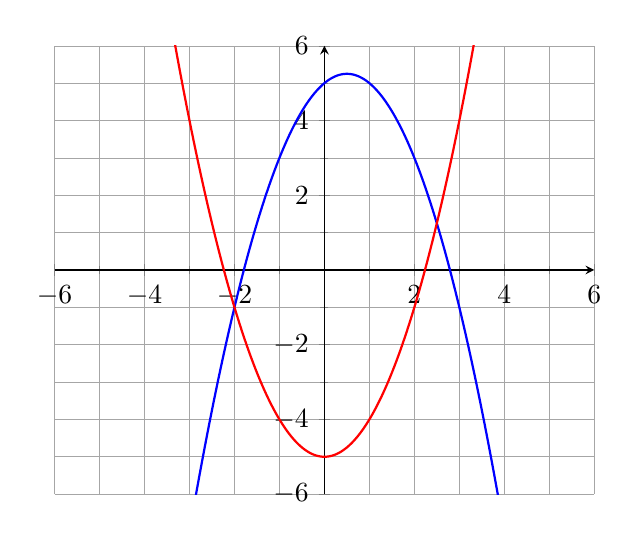
\begin{tikzpicture}
     \begin{axis}%
    [grid=both,
    ymin=-6, ymax=6,
    xmin=-6, xmax=6,
     minor tick num=1,
     grid style={line width=.2pt, draw=gray!70},
     major grid style={line width=.2pt,draw=gray!70},
     axis lines=middle,
     enlargelimits=false
    ]
    \addplot+[blue,mark=none,thick,samples=400] {-x^2+x+5};
    \addplot+[red,mark=none,thick,samples=400] {x^2-5};
  \end{axis}
\end{tikzpicture}
\end{center}
\end{exercise}
\begin{solution}[2in]

\end{solution}

\newpage

\subsection{Domains of Compositions}

Here is a nice visualization of compositions to understand their domains.

\ifprintanswers
\else
\vspace{4in}
\fi

\begin{fact}
If we have two functions $f(x)$ and $g(x)$ with $D_f$ and $D_g$ their
respective domains, then the domain of $(f\circ g)(x)$ is
\[
D_{f\circ g}=\blank{D_g\cap\{x\mid g(x)
\text{ is in }D_f\}}{D_g\cap\{x\mid g(x)\text{ is in }D_f\}}
\]
\end{fact}

\begin{exercise}
Find the domain of $(f\circ g)(x)$ when
\[
f(x)=\frac{1}{8x-16}\quad\&\quad g(x)=\sqrt{2x+10}
\]
\end{exercise}
\begin{solution}[2.5in]

\end{solution}

\begin{exercise}
Find the domain of $f(g(x))$ when
\[
f(x)=\frac{4}{x+2}\quad\&\quad g(x)=\frac{-2}{3x-2}
\]
\end{exercise}
\begin{solution}[2.5in]

\end{solution}

\subsection{Decomposing functions}

\begin{exercise}
Find $f(x)$ and $g(x)$ such that
\[
(f\circ g)(x)=\sqrt{x^2+1}
\]
\end{exercise}
\begin{solution}[3in]

\end{solution}

\newpage

\begin{exercise}
For $\dl h(x)=\frac{-5}{(-x-3)^9}$, find $f(x)$ and $g(x)$ such that
$f(g(x))=h(x)$.
\end{exercise}
\begin{solution}[3in]

\end{solution}

%!TEX root = main.tex
%%% Polynomials
\part{}

\section{Quadratics \& Their Applications}

\begin{ques}
What is a quadratic's graph?
\end{ques}

\ifprintanswers
\else
\begin{center}

\begin{tikzpicture}[scale=0.4]
\draw[step=1cm,gray,very thin] (-7,-7) grid (7,7);
\draw (-7,0) -- (7,0);
\draw (0,-7) -- (0,7);
\end{tikzpicture}
\hspace{1in}

\begin{tikzpicture}[scale=0.4]
\draw[step=1cm,gray,very thin] (-7,-7) grid (7,7);
\draw (-7,0) -- (7,0);
\draw (0,-7) -- (0,7);
\end{tikzpicture}
\end{center}
\fi

We call these shapes \blank{parabolas}{parabolas}.

\subsection{Standard form}

\begin{definition}\label{def: std form parabola}
The following is the \emph{standard form} of a parabola with \emph{vertex} $(h,k)$:
\[
f(x)=\blank{a(x-h)^2+k}{a(x-h)^2+k}
\]
If $\blank{a>0}{a>0}$ then the quadratic opens up,
and if $\blank{a<0}{a<0}$ then the quadratic opens
down. We call $\blank{x=h}{x=h}$ the \emph{axis of symmetry}.
\end{definition}

\subsubsection*{Basic quadratic}

\ifprintanswers
\else
\begin{center}
\raisebox{-6em}{
\begin{tikzpicture}[scale=0.4]
\draw[step=1cm,gray,very thin] (-7,-7) grid (7,7);
\draw (-7,0) -- (7,0);
\draw (0,-7) -- (0,7);
\end{tikzpicture}}
\hspace{1in}
\begin{tabular}{rl}
Vertex: & $\blank{(0,0)}{(0,0)}$\\
Axis of Symmetry: & $\blank{x=0}{x=0}$\\
Scale: & $\blank{a=1}{a=1}$
\end{tabular}
\end{center}
\fi

\ifprintanswers\else\newpage\fi

\begin{exercise}
Graph $f(x)=(x-2)^2+1$ below.
\end{exercise}

\ifprintanswers
\else
\begin{center}
\begin{tikzpicture}[scale=0.4]
\draw[step=1cm,gray,very thin] (-7,-7) grid (7,7);
\draw (-7,0) -- (7,0);
\draw (0,-7) -- (0,7);
\end{tikzpicture}
\end{center}
\fi

\vspace{0.5em}

\begin{exercise}
Graph $f(x)=-2(x-1)^2+2$ below.
\end{exercise}

\ifprintanswers
\else
\begin{center}
\begin{tikzpicture}[scale=0.4]
\draw[step=1cm,gray,very thin] (-7,-7) grid (7,7);
\draw (-7,0) -- (7,0);
\draw (0,-7) -- (0,7);
\end{tikzpicture}
\end{center}
\fi

\vspace{0.5em}

\subsection{General form}

\begin{definition}\label{def: gen form quadratic}
The \emph{general form} of a quadratic is as follows:
\[
f(x)=\blank{ax^2+bx+c}{ax^2+bx+c}
\]
\begin{itemize}
\item Vertex: $\blank{\left(\frac{-b}{2a},f\left(\frac{-b}{2a}\right)\right)}{\left(\frac{-b}{2a},f\left(\frac{-b}{2a}\right)\right)}$
\item Axis of Symmetry: $\blank{x=\frac{-b}{2a}}{x=\frac{-b}{2a}}$.
\end{itemize}
\end{definition}

So standard form is good for graphing, but we tend to see most quadratics in general form.
As such, we will need to be able to change between the two forms.

\ifprintanswers\else\newpage\fi

\begin{exercise}
What is the standard form of
\[
f(x)=x^2-4x+2
\]
\end{exercise}
\begin{solution}[3.5in]

\end{solution}

\vspace{0.5em}

\begin{exercise}
Write $f(x)=2x^2+12x+3$ in standard form.
\end{exercise}
\begin{solution}[4in]

\end{solution}

\vspace{0.5em}

\subsection{Determining the equation from the graph}

\begin{exercise}
Find the equation of the following parabola in both standard and general form:
\begin{center}
\begin{tikzpicture}
     \begin{axis}%
    [grid=both,
    ymin=-6, ymax=6,
    xmin=-6, xmax=6,
     minor tick num=1,
     grid style={line width=.1pt, draw=gray!30},
     major grid style={line width=.2pt,draw=gray!50},
     axis lines=middle,
     enlargelimits=false,
     domain=-6:6,
     samples=100
    ]
    \addplot+[blue,mark=none,thick] {-2*x^2 -12*x-14};
  \end{axis}
\end{tikzpicture}
\end{center}
\end{exercise}
\begin{solution}[3.5in]

\end{solution}

\ifprintanswers\else\newpage\fi

\begin{exercise}
Find both the standard and general form of $f(x)$ below:
\begin{center}
\begin{tikzpicture}
     \begin{axis}%
    [grid=both,
    ymin=-6, ymax=6,
    xmin=-6, xmax=6,
     minor tick num=1,
     grid style={line width=.1pt, draw=gray!30},
     major grid style={line width=.2pt,draw=gray!50},
     axis lines=middle,
     enlargelimits=false,
     domain=-6:6,
     samples=100
    ]
    \addplot+[blue,mark=none,thick] {x^2 -8*x+18};
  \end{axis}
\end{tikzpicture}
\end{center}
\end{exercise}
\begin{solution}[3.5in]

\end{solution}

\ifprintanswers\else\newpage\fi

\subsection{Using intercepts to find the equation}

Sometimes the vertex is not a nice point that we can see, but the intercepts
are nice such as the following problem:

\vspace{0.5em}

\begin{exercise}
Find the general form of $f(x)$ below:
\begin{center}
\begin{tikzpicture}
     \begin{axis}%
    [grid=both,
    ymin=-6, ymax=6,
    xmin=-6, xmax=6,
     minor tick num=1,
     grid style={line width=.1pt, draw=gray!30},
     major grid style={line width=.2pt,draw=gray!50},
     axis lines=middle,
     enlargelimits=false,
     domain=-6:6,
     samples=100
    ]
    \addplot+[blue,mark=none,thick] {x^2+x-2};
  \end{axis}
\end{tikzpicture}
\end{center}
\end{exercise}
\begin{solution}[3.5in]

\end{solution}

\subsection{Finding domain \& range from equations}

\ifprintanswers
\else
\begin{center}
\raisebox{-6em}{\begin{tikzpicture}[scale=0.4]
\draw[step=1cm,gray,very thin] (-7,-7) grid (7,7);
\draw (-7,0) -- (7,0);
\draw (0,-7) -- (0,7);
\end{tikzpicture}}
\hspace{1in}
\begin{tabular}{rl}
Domain: & $\blank{(-\infty,\infty)}{(-\infty\infty)}$\\
(if $a>0$) Range: & $\blank{[k,\infty)}{[k,\infty)}$\\
(if $a<0$) Range: & $\blank{(-\infty,k]}{(-\infty,k]}$
\end{tabular}
\end{center}
\fi

\begin{exercise}
Find the domain and range of $f(x)=(x+3)^2-4$
\end{exercise}
\begin{solution}[2in]

\end{solution}

\vspace{0.5em}

\begin{exercise}
Find the domain and range of $f(x)=-3x^2+12x+17$
\end{exercise}
\begin{solution}[3.5in]

\end{solution}

\subsection{Finding intercepts from the equation}

\begin{exercise}
Find the $x$- and $y$-intercepts of $f(x)=2x^2-4x-6$.
\end{exercise}
\begin{solution}[3in]

\end{solution}

\subsection{Maximum and Minimum values of quadratics}

\begin{note}
The max/min value always occur at the \blank{$y$ value of the vertex}{$y$ value of the vertex}.
\begin{itemize}
    \item If $a>0$ it has a \blank{minimum value}{minimum value},
    \item and if $a<0$ it has a \blank{maximum value}{maximum value}.
\end{itemize}
\end{note}

\begin{exercise}
A farmer is building a fence to enclose a rectangular area next to a wall.
They have 164 ft of fence to use. What is the largest area they can enclose in fence?
\end{exercise}
\begin{solution}[3in]

\end{solution}

\begin{exercise}
Find the dimensions with the maximum area that is fenced in using the shape below and using 234 ft of fence.
\begin{center}
\begin{tikzpicture}
\draw (0,0) -- (6,0) -- (6,3) -- (0,3) -- cycle;
\draw (3,0) -- (3,3);
\end{tikzpicture}  
\end{center}

\end{exercise}
\begin{solution}[2in]

\end{solution}

\section{Polynomials}

\begin{definition}\label{def: power function}
A \emph{power function} is a function that can be written as
\[
f(x)=\blank{kx^n}{kx^n}
\]
\end{definition}
\begin{example}
\text{}
\begin{itemize}
    \item $\blank{f(x)=3x^2}{f(x)=3x^2}$
    \item $\blank{f(x)=7\sqrt[3]{x}=7x^{1/3}}{f(x)=7\sqrt[3]{x}=7x^{1/3}}$
\end{itemize}
\end{example}

\begin{nonex}
\text{}
\begin{itemize}
    \item $\blank{f(x)=5\cdot3^x}{f(x)=5\cdot3^x}$
    \item $\blank{f(x)=2x^2+7x}{f(x)=2x^2+7x}$
\end{itemize}
\end{nonex}

Having defined polynomials before (see Definition \ref{def: polynomial}), we can define them sightly differently using power functions as follows:

\begin{definition}\label{def: polynomial 2}
A \emph{polynomial} is a sum of power functions such that all of the powers are natural numbers (non-negative integers) with the following 
form:
\[
f(x)=a_nx^n+a_{n-1}x^{n-1}+\cdots+a_1x+a_0.
\]
\end{definition}

Recall that $a_n$ is called the leading coefficient, $a_nx^n$
is the leading term and $n$ is the degree of $f(x)$.

\vspace{0.5em}

\begin{example}
\text{}
\begin{itemize}
    \item $\blank{f(x)=3x^2}{f(x)=3x^2}$
    \item $\blank{f(x)=2x^2+7x}{f(x)=2x^2+7x}$
    \item $\blank{f(x)=5x^7+3x^2-4}{f(x)=5x^7+3x^2-4}$
\end{itemize}
\end{example}

\vspace{0.5em}

\begin{nonex}
\text{}
\begin{itemize}
    \item $\blank{f(x)=3x^2+7x^{1/2}}{f(x)=3x^2+7x^{1/2}}$
\end{itemize}
\end{nonex}

\subsection{Graphs of Polynomials}

The graphs of polynomials have 3 key properties:
\begin{enumerate}[1)]
    \item \blank{smooth}{smooth} - the graph has no sharp corners.
    \item \blank{continuous}{continuous} - no jumps or breaks in the graph.
    \item \blank{No Asymptotes}{No Asymptotes}
\end{enumerate}

\begin{ques}
What is an \blank{asymptote}{asymptote}?
\end{ques}

\begin{itemize}
    \item \blank{Vertical Asymptotes (VA)}{Vertical Asymptotes (VA)} - 
    vertical lines that a function approaches by cannot cross.
    \item \blank{Horizontal Asymptotes (HA)}{Horizontal Asymptotes (HA)} - horizontal lines that a function approaches as $x\rightarrow\infty$ or $x\rightarrow-\infty$.
\end{itemize}

\ifprintanswers\else\newpage\fi

Here are some visualizations of these different properties:

\vspace{2em}

\ifprintanswers
\else
\begin{center}
\begin{tikzpicture}[scale=0.5]
\draw[step=1cm,gray,very thin] (-5,-5) grid (5,5);
\draw (-5,0) -- (5,0);
\draw (0,-5) -- (0,5);
\end{tikzpicture}
\hspace{1in}
\begin{tikzpicture}[scale=0.5]
\draw[step=1cm,gray,very thin] (-5,-5) grid (5,5);
\draw (-5,0) -- (5,0);
\draw (0,-5) -- (0,5);
\end{tikzpicture}
\end{center}
\vspace{1em}
\begin{center}
\begin{tikzpicture}[scale=0.5]
\draw[step=1cm,gray,very thin] (-5,-5) grid (5,5);
\draw (-5,0) -- (5,0);
\draw (0,-5) -- (0,5);
\end{tikzpicture}
\hspace{1in}
\begin{tikzpicture}[scale=0.5]
\draw[step=1cm,gray,very thin] (-5,-5) grid (5,5);
\draw (-5,0) -- (5,0);
\draw (0,-5) -- (0,5);
\end{tikzpicture}
\end{center}
\fi

\ifprintanswers\else\newpage\fi

\begin{exercise}
Which of the following are polynomials?
\begin{center}
\raisebox{10em}{(A) }
\begin{tikzpicture}[scale=0.75]
     \begin{axis}%
    [grid=both,
     minor tick num=4,
     ymin=-4, ymax=10,
     xmin=-6, xmax=6,
     grid style={line width=.1pt, draw=gray!30},
     major grid style={line width=.2pt,draw=gray!50},
     axis lines=middle,
     enlargelimits=false,
     samples=100
    ]
    \addplot+[blue,mark=none,thick] {(x-0.5)*(x+1.5)*(x-1.5)*(x+2.5)};
  \end{axis}
\end{tikzpicture}
\hspace{1in}
\raisebox{10em}{(B) }
\begin{tikzpicture}[scale=0.75]
     \begin{axis}%
    [grid=both,
     minor tick num=4,
     ymin=-4, ymax=10,
     grid style={line width=.1pt, draw=gray!30},
     major grid style={line width=.2pt,draw=gray!50},
     axis lines=middle,
     enlargelimits=false,
     samples=200
    ]
    \addplot+[blue,mark=none,thick] {x/((x+2)*(x+2)*(x-2)*(x-2))};
  \end{axis}
\end{tikzpicture}
\end{center}
\vspace{1em}
\begin{center}
\raisebox{10em}{(C) }
\begin{tikzpicture}[scale=0.75]
     \begin{axis}%
    [grid=both,
     minor tick num=4,
     ymin=-4, ymax=10,
     xmin=-6, xmax=6,
     grid style={line width=.1pt, draw=gray!30},
     major grid style={line width=.2pt,draw=gray!50},
     axis lines=middle,
     enlargelimits=false,
     samples=200
    ]
    \addplot+[blue,mark=none,thick] {3^x};
  \end{axis}
\end{tikzpicture}
\hspace{1in}
\raisebox{10em}{(D) }
\begin{tikzpicture}[scale=0.75]
     \begin{axis}%
    [grid=both,
     minor tick num=4,
     ymin=-4, ymax=10,
     xmin=-6, xmax=6,
     grid style={line width=.1pt, draw=gray!30},
     major grid style={line width=.2pt,draw=gray!50},
     axis lines=middle,
     enlargelimits=false,
     samples=200
    ]
    \addplot+[blue,mark=none,thick] {x*(x-2)*(x+3)};
  \end{axis}
\end{tikzpicture}
\end{center}
\end{exercise}

\subsection{End behavior of a polynomial}

The end behavior of a polynomial describes what $f(x)$ is 
doing as $x\rightarrow\blank{\infty}{\infty}$ or\\ $x\rightarrow\blank{-\infty}{-\infty}$.

\vspace{0.5em}

\begin{ques}
What do we need from a polynomial's equation to determine the end behavior?
\end{ques}

\vspace{0.5em}

\begin{prop}
If $f(x)=a_nx^n+a_{n-1}^{n-1}+\cdots$, then the end behavior of $f(x)$ can be
categorized as follows:
\begin{center}
\begin{tabular}{c|c|c}
 & $n$ even  & $n$ odd \\\hline
$a_n>0$ & \phantom{$\dl==\Bigg(\frac{A}{B}==$} & \phantom{$\dl===\Bigg(\frac{A}{B}==$}  \\\hline
$a_n<0$ & \phantom{$\dl===\Bigg(\frac{A}{B}==$}  & \phantom{$\dl===\Bigg(\frac{A}{B}==$} 
\end{tabular}
or
\begin{tabular}{c|c|c}
 & $n$ even  & $n$ odd \\\hline
$a_n>0$ & \phantom{$\dl===\Bigg(\frac{A}{B}==$} & \phantom{$\dl===\Bigg(\frac{A}{B}==$}  \\\hline
$a_n<0$ & \phantom{$\dl===\Bigg(\frac{A}{B}==$}  & \phantom{$\dl===\Bigg(\frac{A}{B}==$} 
\end{tabular}
\end{center}
\end{prop}

\ifprintanswers\else\newpage\fi

\begin{exercise}
What is the end behavior of $f(x)=18x^3+2$
\end{exercise}
\begin{solution}[1in]

\end{solution}

\vspace{0.5em}

\begin{exercise}
Describe the end behavior of
\[
f(x)=-5x(x-4)(x+5)(2x+3)
\]
\end{exercise}
\begin{solution}[1in]

\end{solution}

\vspace{0.5em}

\begin{exercise}
Which of the following factors would cause the graph of $f(x)$ to decrease
as $x$ goes to negative infinity?
\[
f(x)=(2x^2+5)(x-7)
\]
\end{exercise}
\begin{checkboxes}
\choice $-3$
\CorrectChoice $5x^2$
\choice $4(2x-7)$
\end{checkboxes}
\begin{solution}[3in]

\end{solution}

\subsection{Identifying intercepts}

Recall that $x$-intercepts are where $\blank{f(x)=0}{f(x)=0}$, and the
$y$-intercept is at $\blank{f(0)}{f(0)}$.

\begin{exercise}
What are the intercepts of
\[
f(x)=(x-5)(x+3)(x-1)
\]
\end{exercise}

\begin{solution}[2in]

\end{solution}

\subsection{Finding zeros}

There are two steps to finding the zeros of a polynomial:
\begin{enumerate}[1)]
    \item \blank{Factor out the GCF (if there is one)}{Factor out the GCF (if there is one)}
    \item \blank{Factor the remaining polynomial}{Factor the remaining polynomial}
\end{enumerate}

\vspace{0.5em}

\begin{exercise}
Find the zeros of $f(x)=x^5-14x^4+49x^3$
\end{exercise}
\begin{solution}[3in]

\end{solution}

\subsection{More on graphs and degrees}

\begin{definition}\label{def: turning point}
A \emph{turning point} is a point where $f(x)$
changes from \blank{increasing to}{increasing to} \blank{decreasing or vice-versa}{decreasing or vice-versa}.
\end{definition}

\begin{center}
\begin{tikzpicture}[scale=0.75]
\draw[step=1cm,gray,very thin] (-5,-5) grid (5,5);
\draw (-5,0) -- (5,0);
\draw (0,-5) -- (0,5);
\end{tikzpicture}
\end{center}

Here are two facts relating to the degree of a polynomial and its graph.

 \begin{fact}
A polynomial of degree $n$ can have at most $\blank{n-1}{n-1}$ turning points.
\end{fact}

\begin{fact}
A polynomial of degree $n$ can have at most $\blank{n}{n}$ $x$-intercepts.
\end{fact}

\begin{exercise}
If a polynomial has $7$ $x$-intercepts, what can you say about the degree?
\end{exercise}
\begin{solution}[1in]

\end{solution}

\begin{exercise}
If the degree of a polynomial is $8$, what can you say about the number of turning points?
\end{exercise}
\begin{solution}[1in]

\end{solution}

\subsection{More about zeros}

What follows is one of the most important theorems in algebra, but we need one definition first.

\begin{definition}
If $b$ is a zero of a polynomial $f(x)$, then the \emph{multiplicity} of $b$ is the number of times that $b$ appears as a zero to $f(x)$.
\end{definition}

\begin{theorem}[Fundamental Theorem of Algebra]\label{thm: FTA}
If we allow complex numbers, then any polynomial can be completely factored into linear
factors of its zeros. That is if $f(x)$ is a polynomial and $b_1,b_2,\ldots,b_k$ are the
zeros of $f(x)$ with multiplicities $m_1,m_2,\ldots,m_k$, we can write $f(x)$ as follows:
\[
f(x)=a(x-b_1)^{m_1}(x-b_2)^{m_2}\cdots(x-b_k)^{m_k}
\]
\end{theorem}

\begin{example}
The polynomial $f(x)=(x-3)^2(x+4)^6$ has zeros at $\blank{x=3}{x=3}$ and
$\blank{x=-4}{x=-4}$ with multiplicities $\blank{2}{2}$ and $\blank{6}{6}$, respectively.
\end{example}

\begin{note}
A consequence of the Fundamental Theorem of Algebra is
\[
m_1+m_2+\cdots+m_k=\blank{\deg(f)}{\deg(f)}
\]
\end{note}

The multiplicities have an effect on how the graph acts around the corresponding
zero ($x$-intercept).

\begin{itemize}
    \item If the multiplicity of the zero $b$ is odd, then 
\begin{center}
\rule{1in}{0.1pt}\quad\text{or}\quad\rule{1in}{0.1pt}
\end{center}
\item If the multiplicity of the zero $b$ is even, then 
\begin{center}
\rule{1in}{0.1pt}\quad\text{or}\quad\rule{1in}{0.1pt}
\end{center}
\end{itemize}

\vspace{0.5em}

Additionally, the flatter the graph is around the zero the larger the multiplicity.

\vspace{0.5em}

Using these ideas we can make conclusions about the multiplicity of zeros based
on the graph of a polynomial and some information about the degree.

\ifprintanswers\else\newpage\fi

\begin{exercise}
Given that $f(x)$ below is a degree 4 polynomial, find
the zeros and their multiplicities:
\begin{center}
\begin{tikzpicture}
\begin{axis}%
    [grid=both,
     minor tick num=1,
     ymin=-6, ymax=6,
     xmin=-6, xmax=6,
     grid style={line width=.1pt, draw=gray!30},
     major grid style={line width=.2pt,draw=gray!50},
     axis lines=middle,
     enlargelimits=false,
     domain=-6:6,
     samples=200
    ]
    \addplot+[blue,mark=none,thick] {1/25*(x-4)^3*(x+2)};
  \end{axis}
\end{tikzpicture}
\end{center}
\end{exercise}
\begin{solution}[3in]

\end{solution}

\subsection{The Intermediate Value Theorem}

\begin{center}
\begin{tikzpicture}[scale=0.75]
\draw[step=1cm,gray,very thin] (-2,-4) grid (8,4);
\draw (-2,0) -- (8,0);
\draw (0,-4) -- (0,4);
\end{tikzpicture}
\end{center}

\begin{theorem}[Intermediate Value Theorem]\label{thm: IVT}
For a continuous function (think polynomial) $f(x)$ on $[a,b]$
and a number $z$ in between $f(a)$ and $f(b)$, there exists a $c$
in $[a,b]$ such that $f(c)=z$.
\end{theorem}

\begin{ques}
Do we care?
\end{ques}

This theorem is useful for \blank{``finding zeros''}{``finding zeros''} because
if $\blank{0}{0}$ is between $f(a)$ and $f(b)$ and $f$ is continuous on $[a,b]$,
then the IVT says that there is a $c$ in $[a,b]$ such that $f(c)=\blank{0}{0}$.


\begin{note}
$\blank{0}{0}$ is between $f(a)$ and $f(b)$ $\Longleftrightarrow$
$f(a)$ and $f(b)$ \blank{have different signs}{have different signs}
\end{note}

\begin{center}
\begin{tikzpicture}[scale=0.5]
\draw[step=1cm,gray,very thin] (-2,-3) grid (8,3);
\draw (-2,0) -- (8,0);
\draw (0,-3) -- (0,3);
\end{tikzpicture}
\end{center}

\begin{exercise}
Show that $f(x)=3x^2-1$ has a zero in $[-1,0]$ using IVT.
\end{exercise}
\begin{solution}[2in]

\end{solution}

\begin{exercise}
Does IVT guarantee that $f(x)=x^2-4x+4$ have a zero between $[1,4]$? 
\end{exercise}
\begin{solution}[2in]

\end{solution}

\subsection{Drawing conclusions from graphs of polynomials}

\begin{exercise}
Describe the leading coefficient and degree of the following polynomial:
\begin{center}
\begin{tikzpicture}[scale=0.75]
\begin{axis}%
    [grid=both,
     minor tick num=1,
     ymin=-6, ymax=6,
     xmin=-6, xmax=6,
     grid style={line width=.1pt, draw=gray!30},
     major grid style={line width=.2pt,draw=gray!50},
     axis lines=middle,
     enlargelimits=false,
     domain=-6:6,
     samples=200
    ]
    \addplot+[blue,mark=none,thick] {1/2*(x-4)*(x+2)*(x-1)};
  \end{axis}
\end{tikzpicture}
\end{center}
\end{exercise}
\begin{solution}[1in]

\end{solution}
\begin{exercise}
Describe the leading coefficient and degree of the following polynomial:
\begin{center}
\begin{tikzpicture}[scale=0.75]
\begin{axis}%
    [grid=both,
     minor tick num=1,
     ymin=-6, ymax=6,
     xmin=-6, xmax=6,
     grid style={line width=.1pt, draw=gray!30},
     major grid style={line width=.2pt,draw=gray!50},
     axis lines=middle,
     enlargelimits=false,
     domain=-6:6,
     samples=200
    ]
    \addplot+[blue,mark=none,thick] {1/15*(x-4)*(x+5)*(x+2)*(x-1)};
  \end{axis}
\end{tikzpicture}
\end{center}
\end{exercise}
\begin{solution}[1in]

\end{solution}

\ifprintanswers\else\newpage\fi

\subsection{Graphing Polynomials}

\begin{exercise}
Graph $f(x)=4(x-2)(x+1)(x+6)$.
\end{exercise}
\ifprintanswers
\else
\begin{center}
\begin{tikzpicture}[scale=0.5]
\draw[step=1cm,gray,very thin] (-8,-8) grid (8,8);
\draw (-8,0) -- (8,0);
\draw (0,-8) -- (0,8);
\end{tikzpicture}
\hspace{3in}\phantom{=}
\end{center}
\fi

\begin{exercise}
Graph $f(x)=-2(x-6)(x-2)(x+3)$.
\end{exercise}
\ifprintanswers
\else
\begin{center}
\begin{tikzpicture}[scale=0.5]
\draw[step=1cm,gray,very thin] (-8,-8) grid (8,8);
\draw (-8,0) -- (8,0);
\draw (0,-8) -- (0,8);
\end{tikzpicture}
\hspace{3in}\phantom{=}
\end{center}
\fi

\ifprintanswers\else\newpage\fi

\subsection{Finding the equation from the graph}

\begin{exercise}
The graph of the polynomial $f(x)$ is given below. If $f(x)$
is degree 3, find the equation of $f(x)$
\begin{center}
\begin{tikzpicture}
\begin{axis}%
    [grid=both,
     minor tick num=1,
     ymin=-6, ymax=6,
     xmin=-6, xmax=6,
     grid style={line width=.1pt, draw=gray!30},
     major grid style={line width=.2pt,draw=gray!50},
     axis lines=middle,
     enlargelimits=false,
     domain=-6:6,
     samples=200
    ]
    \addplot+[blue,mark=none,thick] {1/3*(x+1)*(x-1)*(x-3)};
  \end{axis}
\end{tikzpicture}
\end{center}
\end{exercise}
\begin{solution}[2in]

\end{solution}

\ifprintanswers\else\newpage\fi

\begin{exercise}
The graph of the polynomial $f(x)$ is given below. If $f(x)$
is degree 4, find the equation of $f(x)$
\begin{center}
\begin{tikzpicture}
\begin{axis}%
    [grid=both,
     minor tick num=1,
     ymin=-6, ymax=6,
     xmin=-6, xmax=6,
     grid style={line width=.1pt, draw=gray!30},
     major grid style={line width=.2pt,draw=gray!50},
     axis lines=middle,
     enlargelimits=false,
     domain=-6:6,
     samples=200
    ]
    \addplot+[blue,mark=none,thick] {1/24*(x+3)*(x+1)*(x-2)*(x-4)};
  \end{axis}
\end{tikzpicture}
\end{center}
\end{exercise}
\begin{solution}[2in]

\end{solution}

\ifprintanswers\else\newpage\fi

\subsection{Finding the equation from key information}

\begin{exercise}
Write a polynomial, $p(x)$, in factored form given the following requirements:
\begin{itemize}
    \item degree 4;
    \item leading coefficient of 1;
    \item has zeros at $(1,0)$, $(-4,0)$, and $(2,0)$;
    \item $y$-intercept is $(0,-24)$.
\end{itemize}
\end{exercise}
\begin{solution}[3in]

\end{solution}

\begin{exercise}
Write a polynomial, $p(x)$, in factored form given the following requirements:
\begin{itemize}
    \item degree 3;
    \item leading coefficient of 1;
    \item has zeros at $(8,0)$, $(-4,0)$, and $(1,0)$;
    \item $y$-intercept is $(0,32)$.
\end{itemize}
\end{exercise}
\begin{solution}[2in]

\end{solution}

\begin{exercise}
Which of the following is the equation of a polynomial of degree 4 with zeros at
$(4,0)$ \& $(3,0)$ and $y$-intercept of $(0,96)$.
\end{exercise}
\begin{checkboxes}
\choice $y=(x+4)(x+3)(x+8)(x+1)$
\choice $y=(x+4)(x-3)(x-2)(x-1)$
\choice $y=(x-4)(x-3)(x+8)(x-1)$
\CorrectChoice $y=(x-4)(x-3)(x+2)(x+4)$
\end{checkboxes}
\begin{solution}[2in]

\end{solution}

\section{Division of Polynomials \& the Remainder Theorem}

\subsection{Long Division}

First I want to recall how we long divide numbers

\begin{exercise}
Use long division to find $24\div2$.
\end{exercise}
\begin{solution}[2in]

\end{solution}

We are now going to do the exact same thing with polynomials

\ifprintanswers\else\newpage\fi

\begin{exercise}
Divide $x^2+14x+45$ by $x+9$.
\end{exercise}
\begin{solution}[3in]

\end{solution}

\begin{exercise}
Divide $24x^3+2x^2-20x-6$ by $4x+3$.
\end{exercise}
\begin{solution}[3in]

\end{solution}

\begin{exercise}
Divide $25$ by $2$.
\end{exercise}
\begin{solution}[2in]

\end{solution}

\begin{exercise}
Divide $40x^2+31x-33$ by $5x+7$.
\end{exercise}
\begin{solution}[4in]

\end{solution}

\vspace{0.5em}

\begin{exercise}
Divide $-60x^3-40x^2+54x+38$ by $6x+4$.
\end{exercise}
\begin{solution}[4in]

\end{solution}

\begin{exercise}
Divide $6x^3-8x+4$ by $2x+6$.
\end{exercise}
\begin{solution}[4in]

\end{solution}

\begin{exercise}
The volume of a hexagonal prism is $12x^5+8x^4+9x^3-42x^2-33x-44$
and the area of the base is $2x^2+3x+4$. Find the height of the
prism.
\end{exercise}
\begin{solution}[4in]

\end{solution}

\subsection{Synthetic division}

This is a way to divide polynomial when the divisor is of the form
$\blank{x-c}{x-c}$

\begin{exercise}
Synthetically divide $x^2+14x+45$ by $x+9$
\end{exercise}
\begin{solution}[2.5in]

\end{solution}

\begin{exercise}
Use synthetic division to find $(x^4-10x^2-13x-50)\div(x+5)$
\end{exercise}
\begin{solution}[2.5in]

\end{solution}

\begin{exercise}
Synthetically divide $x^4-2x^2-4x-48$ by $x-3$
\end{exercise}
\begin{solution}[2.5in]

\end{solution}

\subsection{The Remainder Theorem}

\begin{theorem}[Remainder Theorem]\label{thm: remainder thm}
If a polynomial $f(x)$ is divided by $x-c$,
then remainder is $\blank{f(c)}{f(c)}$.
\end{theorem}

\begin{exercise}
What is the remainder of $g(x)=3x^3-20x^2+29x+30$ divided
by $x+2$
\end{exercise}
\begin{solution}[2in]

\end{solution}

\subsection{The Factor Theorem}

\begin{theorem}[Factor Theorem]\label{thm: factor thm}
$x-c$ is a factor of $f(x)$ if and only if
the remainder of $f(x)$ when divided by $x-c$ is $\blank{0}{0}$.

\vspace{0.5em}

Another way we can say this is $x-c$ is a factor of $f(x)$
if and only if $\blank{f(c)=0}{f(c)=0}$.
\end{theorem}

\begin{exercise}
Consider $f(x)=x^3-4x^2-47x+210$. When $f(x)$ is divided by $x+7$,
the remainder is $0$. What other binomials have a reminder of zero?
\end{exercise}
\begin{solution}[3.5in]

\end{solution}

\vspace{0.5em}

\begin{exercise}
For what values of $x$ is $x^3-12x^2+39x-28=0$?
\end{exercise}
\begin{solution}[4in]

\end{solution}

\section{Zeros of Polynomials}

First we need a rule for guessing zeros.

\subsection{Rational zero theorem}

\begin{theorem}[Rational Zero Theorem]\label{thm: rational zero thm}
If $f(x)=a_nx^n+a_{n-1}x^{n-1}+\cdots+a_1x+a_0$ has integer
coefficients, then every rational zero (fraction zero) of $f(x)$
is of the form $\dl\frac{p}{q}$, where $p$ is a factor
$\blank{a_0 (\text{the constant})}{a_0 (\text{the constant})}$ and
$q$ is a factor of $\blank{a_n (\text{the leading coefficient})}{a_n (\text{the leading coefficient})}$
\end{theorem}

\begin{exercise}
What are the possible rational zeros of $4x^5+12x^4-x-3$
\end{exercise}
\begin{solution}[1.5in]

\end{solution}

\begin{exercise}
What are the possible rational zeros of $x^3+2x^2-5x-6$
\end{exercise}
\begin{solution}[1in]

\end{solution}

\begin{exercise}
Find the rational zeros of $f(x)=x^3-5x^2-33x-27$.
\end{exercise}
\begin{solution}[3in]

\end{solution}

\subsection{Polynomials with complex zeros}

\begin{exercise}
Find all of the zeros of $f(x)=x^3+13x^2+57x+85$.
\end{exercise}
\begin{solution}[2in]

\end{solution}

\ifprintanswers\else\newpage\fi

\subsection{Linear Factorization Theorem}

\begin{theorem}[Linear Factorization Theorem]
Any polynomial $f(x)$ can be written as
\[
f(x)=\blank{a_n(x-c_1)(x-c_2)\cdots(x-c_n)}{a_n(x-c_1)(x-c_2)\cdots(x-c_n)}
\]
where $a_n$ is the leading coefficient, the degree of $f(x)$ is $n$,
and $c_1,c_2,\ldots,c_n$ are the complex zeros of $f(x)$ (not necessarily distinct).
\end{theorem}

\begin{exercise}
Find a third degree polynomial that has an output of $16$ when $x=2$
and zeros of $1$ and $-2i$.
\end{exercise}
\begin{solution}[4in]

\end{solution}

\ifprintanswers\else\newpage\fi

\begin{exercise}
Find a third degree polynomial that has an output of $20$ when $x=0$
and zeros of $4$ and $-1+3i$.
\end{exercise}
\begin{solution}[6in]

\end{solution}

\subsection{Descartes' Rule of Signs}

The following is occasionally useful when guessing zeros for the rational zero theorem.

\begin{prop}
\text{}
\begin{enumerate}[1)]
    \item The number of positive real zeros of a polynomial $f(x)$
    is either the number of sign changes of $\blank{f(x)}{f(x)}$
    or less a positive even integer.
    \item The number of negative real zeros of a polynomial $f(x)$
    is either the number of sign changes of $\blank{f(-x)}{f(-x)}$
    or less a positive even integer.
\end{enumerate}
\end{prop}

\vspace{1em}

\begin{exercise}
For $f(x)=7x^4+2x^3+4x^2-6x+5$, what are the possible combinations of positive, negative, and imaginary zeros of $f(x)$.
\end{exercise}
\begin{solution}[2.5in]

\end{solution}

\begin{exercise}
For $f(x)=x^4-2x^3+4x^2-3x+17$, what are the possible combinations of positive, negative, and imaginary zeros of $f(x)$.
\end{exercise}
\begin{solution}[2.5in]

\end{solution}

\begin{exercise}
For $f(x)=x^6-2x^5+7x^4+5x^3-7x^2+3x-10$, what are the possible combinations of positive, negative, and imaginary zeros of $f(x)$.
\end{exercise}
\begin{solution}[2.5in]

\end{solution}


\section{Rational Functions}

\begin{align*}
\text{rational numbers}&\longleftrightarrow\text{fractions of integers}\\
\text{rational functions}&\longleftrightarrow\blank{\text{fractions of polynomials}}{\text{fraction of polynomials}}
\end{align*}

\begin{definition}\label{def: rational functions}
A function $f(x)$ is a \emph{rational function} if
\[
f(x)=
\]
where $p(x)$ and $q(x)$ are \blank{polynomials}{polynomials}
\end{definition}

\begin{example}
\text{}
\begin{itemize}
    \item $\dl\blank{f(x)=\frac{3x+2}{5x^2-7x+1}}{f(x)=\frac{3x+2}{5x^2-7x+1}}$
    \item $\dl\blank{f(x)=\frac{x^7+x-3}{x^2+2x+3}}{f(x)=\frac{x^7+x-3}{x^2+2x+3}}$
\end{itemize}
\end{example}

\begin{nonex}
\text{}
\begin{itemize}
\item $\blank{g(x)=\frac{3x+2}{\sqrt{3x+7}}}{g(x)=\frac{3x+2}{\sqrt{3x+7}}}$
\end{itemize}
\end{nonex}

\begin{note}
Here is some useful notation that we will see when working with rational functions:
\begin{itemize}
    \item $\blank{x\rightarrow a^+}{x\rightarrow a^+}$ - $x$ approaches $a$ from the right/above.
    \item $\blank{x\rightarrow a^-}{x\rightarrow a^-}$ - $x$ approaches $a$ from the left/below.
    \item $\blank{x\rightarrow\infty}{x\rightarrow\infty}$ - $x$ approaches infinity.
    \item $\blank{x\rightarrow-\infty}{x\rightarrow-\infty}$ - $x$ approaches negative infinity.
\end{itemize}
\end{note}

\begin{definition}
A \emph{vertical asymptote} (VA) is a vertical line
$x=a$ such that $f(x)\rightarrow\blank{\pm\infty}{\pm\infty}$ as
$x\rightarrow\blank{a^{\pm}}{a^{\pm}}$
\end{definition}

\ifprintanswers
\else
\begin{center}
\begin{tikzpicture}[scale=0.4]
\draw[step=1cm,gray,very thin] (-5,-5) grid (5,5);
\draw (-5,0) -- (5,0);
\draw (0,-5) -- (0,5);
\end{tikzpicture}
\hspace{0.25in}
\begin{tikzpicture}[scale=0.4]
\draw[step=1cm,gray,very thin] (-5,-5) grid (5,5);
\draw (-5,0) -- (5,0);
\draw (0,-5) -- (0,5);
\end{tikzpicture}
\hspace{0.25in}
\begin{tikzpicture}[scale=0.4]
\draw[step=1cm,gray,very thin] (-5,-5) grid (5,5);
\draw (-5,0) -- (5,0);
\draw (0,-5) -- (0,5);
\end{tikzpicture}
\end{center}
\fi

\ifprintanswers\else\newpage\fi

\begin{definition}
A \emph{horizontal asymptote} (HA) is a horizontal line
$y=b$ such that $f(x)\rightarrow\blank{b^{\pm}}{b^{\pm}}$ as
$x\rightarrow\blank{\pm\infty}{\pm\infty}$
\end{definition}

\ifprintanswers
\else
\begin{center}
\begin{tikzpicture}[scale=0.4]
\draw[step=1cm,gray,very thin] (-5,-5) grid (5,5);
\draw (-5,0) -- (5,0);
\draw (0,-5) -- (0,5);
\end{tikzpicture}
\hspace{0.25in}
\begin{tikzpicture}[scale=0.4]
\draw[step=1cm,gray,very thin] (-5,-5) grid (5,5);
\draw (-5,0) -- (5,0);
\draw (0,-5) -- (0,5);
\end{tikzpicture}
\hspace{0.25in}
\begin{tikzpicture}[scale=0.4]
\draw[step=1cm,gray,very thin] (-5,-5) grid (5,5);
\draw (-5,0) -- (5,0);
\draw (0,-5) -- (0,5);
\end{tikzpicture}
\end{center}
\fi

\subsection{Describe the behavior of rational functions using their graph}

\begin{exercise}
Describe the behavior of $f(x)$ below:
\begin{center}
\begin{tikzpicture}
\begin{axis}%
    [grid=both,
     minor tick num=1,
     ymin=-6, ymax=6,
     xmin=-6, xmax=6,
     grid style={line width=.1pt, draw=gray!30},
     major grid style={line width=.2pt,draw=gray!50},
     axis lines=middle,
     enlargelimits=false,
    ]
    \addplot+[blue,mark=none,thick,samples=800,restrict y to domain=-10:10,domain=-6:6] {(x+5)/(x+3)};
\end{axis}
\end{tikzpicture}
\end{center}
\end{exercise}
\begin{solution}[2in]

\end{solution}

\ifprintanswers\else\newpage\fi

\begin{exercise}
Describe the behavior of $f(x)$ below:
\begin{center}
\begin{tikzpicture}
\begin{axis}%
    [grid=both,
     minor tick num=1,
     ymin=-6, ymax=6,
     xmin=-6, xmax=6,
     grid style={line width=.1pt, draw=gray!30},
     major grid style={line width=.2pt,draw=gray!50},
     axis lines=middle,
     enlargelimits=false,
    ]
    \addplot+[blue,mark=none,thick,samples=800,restrict y to domain=-10:10,domain=-6:6] {((2*x+1)*(x-3))/((x+2)*(x-4))};
\end{axis}
\end{tikzpicture}
\end{center}
\end{exercise}
\begin{solution}[2in]

\end{solution}

\subsection{Finding vertical asymptotes}

\begin{fact}
The function $\dl f(x)=\frac{p(x)}{q(x)}$ has a VA at $x=a$
if \blank{$p(a)\neq0$ and $q(a)=0$}{$p(a)\neq0$ and $q(a)=0$}.

\vspace{1em}

If both \blank{$p(a)=0$ and $q(a)=0$}{$p(a)=0$ and $q(a)=0$}, then
either $a$ is a \blank{removable discontinuity/singularity}{removable discontinuity/singularity} if we can simplify $f(x)$ such
that $a$ no longer makes the denominator \blank{$0$}{$0$}.

\vspace{1em}

If the denominator is still \blank{$0$}{$0$}, but the numerator is not, then it is a VA and is called an \blank{essential singularity}{essential singularity}.
\end{fact}

\ifprintanswers\else\newpage\fi

\begin{exercise}
Consider
\[
f(x)=\frac{x^3-x^2-2x}{x^2+x}.
\]
Does $f(x)$ have any removable discontinuities?
\end{exercise}
\begin{solution}[3.5in]

\end{solution}

\begin{exercise}
Consider
\[
f(x)=\frac{x^2-36}{x^3-2x^2-24x}.
\]
What are the vertical asymptotes of $f(x)$ (if any)?
\end{exercise}
\begin{solution}[3.5in]

\end{solution}

\subsection{Finding horizontal asymptotes}

\begin{fact}
Let $\dl f(x)=\frac{a_nx^n+\cdots+a_1x+a_0}{b_mx^m+\cdots+b_1x+b_0}$.
To find the horizontal asymptote we need to compare the degrees $m$ and $n$:
\begin{itemize}
\item \blank{$n>m$}{$n>m$} $\Rightarrow$ there is no HA.
\item \blank{$n<m$}{$n<m$} $\Rightarrow$ the $x$-axis $(y=0)$
is the HA.
\item \blank{$n=m$}{$n=m$} $\Rightarrow$ $\dl y=\frac{a_n}{b_m}$
is the HA.
\end{itemize}
\end{fact}

\begin{exercise}
What is the HA (if one) of
\[
f(x)=\frac{9x}{3x+1}
\]
\end{exercise}
\begin{solution}[1in]

\end{solution}

\begin{exercise}
What is the HA (if one) of
\[
g(x)=\frac{7x^5+4}{3x^6+x+3}
\]
\end{exercise}
\begin{solution}[1in]

\end{solution}

\begin{exercise}
What is the HA (if one) of
\[
h(x)=\frac{x^2+1}{x+1}
\]
\end{exercise}
\begin{solution}[1in]

\end{solution}

\ifprintanswers\else\newpage\fi

As we saw, some rational functions do not have a HA, but some have the following instead

\begin{definition}\label{def: SA}
If $\dl f(x)=\frac{p(x)}{q(x)}$ is a rational function and
$\deg(p(x))=\deg(q(x))+1$, then $f(x)$ has a \emph{slant asymptote} (SA)
which is a line $y=mx+b$ that $f(x)$ approaches as $x\rightarrow\blank{\pm\infty}{\pm\infty}$
\end{definition}

\begin{ques}
How do you find a SA?
\end{ques}

We use division! Since the denominator's degree is one less than the numerator's degree the quotient will have to have degree 1.

\begin{exercise}
If
\[
h(x)=\frac{x^2+1}{x+1}
\]
what is its SA?
\end{exercise}
\begin{solution}[2in]

\end{solution}

\subsection{Graphing rational functions}

Here is the general strategy if $\dl f(x)=\frac{p(x)}{q(x)}$
is fully simplified.

\begin{enumerate}[1)]
    \item Find the $y$-intercept (if there is one) by finding $\blank{f(0)}{f(0)}$.
    \item Find $x$-intercept (if any) by solving $\blank{p(x)=0}{p(x)=0}$.
    \item Find VA by solving $\blank{q(x)=0}{q(x)=0}$.
    \item Find HA (if there is one) by comparing degrees.
    \begin{enumerate}[4.5)]
        \item Find the SA (if there is one) using division.
    \end{enumerate}
    \item Plot extra points between the intercepts and VA as needed.
\end{enumerate}

\ifprintanswers\else\newpage\fi

\begin{exercise}
Graph $\dl f(x)=\frac{x-1}{x-4}$
\end{exercise}
\ifprintanswers
\else
\begin{center}
\begin{tikzpicture}[scale=0.5]
\draw[step=1cm,gray,very thin] (-8,-8) grid (8,8);
\draw (-8,0) -- (8,0);
\draw (0,-8) -- (0,8);
\end{tikzpicture}
\end{center}
\fi
\begin{solution}[2in]

\end{solution}

\ifprintanswers\else\newpage\fi

\begin{exercise}
Graph $\dl f(x)=\frac{(x-2)(x-5)}{(x-3)^2}$
\end{exercise}
\ifprintanswers
\else
\begin{center}
\begin{tikzpicture}[scale=0.5]
\draw[step=1cm,gray,very thin] (-8,-8) grid (8,8);
\draw (-8,0) -- (8,0);
\draw (0,-8) -- (0,8);
\end{tikzpicture}
\end{center}
\fi
\begin{solution}[4in]

\end{solution}

\ifprintanswers\else\newpage\fi

\subsection{Identifying rational functions from their graphs}

\begin{exercise}
Identify the rational function graphed below. Note the $x$-intercept of $x=-3$ and $(-1,-2)$ is a point on the graph.
\begin{center}
\begin{tikzpicture}
\begin{axis}%
    [grid=both,
     minor tick num=1,
     ymin=-6, ymax=6,
     xmin=-6, xmax=6,
     grid style={line width=.1pt, draw=gray!30},
     major grid style={line width=.2pt,draw=gray!50},
     axis lines=middle,
     enlargelimits=false,
    ]
    \addplot+[blue,mark=none,thick,samples=800,restrict y to domain=-10:10,domain=-6:6] {(x+3)/(x*(x+2))};
\end{axis}
\end{tikzpicture}
\end{center}
\end{exercise}
\begin{solution}[2in]

\end{solution}

\ifprintanswers\else\newpage\fi

\begin{exercise}
Identify the rational function graphed below. Note the $x$-intercept of $x=3$ and $y$-intercept at $-3$.
\begin{center}
\begin{tikzpicture}
\begin{axis}%
    [grid=both,
     minor tick num=1,
     ymin=-6, ymax=6,
     xmin=-6, xmax=6,
     grid style={line width=.1pt, draw=gray!30},
     major grid style={line width=.2pt,draw=gray!50},
     axis lines=middle,
     enlargelimits=false,
    ]
    \addplot+[blue,mark=none,thick,samples=800,restrict y to domain=-10:10,domain=-6:6] {4*(x-3)/((x-2)^2)};
\end{axis}
\end{tikzpicture}
\end{center}
\end{exercise}
\begin{solution}[2in]

\end{solution}

\newpage

\section{Polynomial and Rational Inequalities}

Just as linear inequalities start with solving the "equation", the same is true of
polynomial and rational inequalities.

\subsection{Polynomial inequalities}

Here is the procedure for solving inequalties such as $f(x)>0,~f(x)<0,~f(x)\geq0,~f(x)\leq0$ where
$f(x)$ is a polynomial:
\begin{enumerate}
    \item Set one side to $\blank{0}{0}$
    \item Solve $\blank{f(x)=0}{f(x)=0}$
    \item Plot those solutions on a \blank{number line}{number line}
    \item Find test values in between these numbers and test to find the \blank{sign}{sign}
    \item Choose correct interval(s) based on original inequality $\blank{>0,\geq0\longleftrightarrow+}{>0,\geq0\longleftrightarrow+}$ and
    $\blank{<0,\leq0\longleftrightarrow-}{<0,\leq0\longleftrightarrow-}$
\end{enumerate}
\vspace{0.5em}

\begin{exercise}
Solve $x^2-x>20$ for $x$. (Give your answer in interval notation)
\end{exercise}
\begin{solution}[3in]

\end{solution}

\ifprintanswers\else\newpage\fi

\begin{exercise}
Solve $2x^2\leq-6x-4$ for $x$. (Give your answer in interval notation)
\end{exercise}
\begin{solution}[4in]

\end{solution}

\vspace{0.5em}

\begin{exercise}
Solve $x^3+3x^2\leq x+3$ for $x$. (Give your answer in interval notation)
\end{exercise}
\begin{solution}[4in]

\end{solution}

\subsubsection*{Position of a free-falling object near earth's surface}

\begin{fact}
The position of a free falling object (in feet) at time $t$ can be described by the following quadratic:
\[
s(t)=\blank{-16t^2+v_0t+s_0}{-16t^2+v_0t+s_0}
\]
where $\blank{v_0}{v_0}$ is the initial velocity and $\blank{s_0}{s_0}$ is the initial position.
\end{fact}

\vspace{0.5em}

\begin{exercise}
Given the following position function, find the interval of time that the object is more than $64$
feet above the ground.
\[
s(t)=-16t^2+80t
\]
\end{exercise}
\begin{solution}[3in]

\end{solution}

\subsection{Rational inequalities}

What follows is the procedure for solving rational inequalities.
\begin{enumerate}
    \item Write the inequality with $0$ on one side
    \item Combine the fractions on the other side as \blank{a single fraction}{a single fraction}
    \item Set the numerator and denominator equal to $\blank{0}{0}$
    \item Plot on number line
    \item Test values
    \item Choose correct interval(s)
\end{enumerate}

\vspace{0.5em}

\begin{exercise}
Solve the following for $x$:
\[
\frac{2x}{x+1}\geq1
\]
\end{exercise}
\begin{solution}[3.5in]

\end{solution}

\begin{exercise}
Solve the following for $x$:
\[
\frac{x-2}{x+2}\leq2
\]
\end{exercise}
\begin{solution}[3.5in]

\end{solution}

\begin{exercise}
Find the solution to the following inequality in interval notation:
\[
\frac{2}{x+3}\leq\frac{1}{x-3}
\]
\end{exercise}
\begin{solution}[3.5in]

\end{solution}

\begin{exercise}
Find the solution to the following inequality in interval notation:
\[
\frac{3}{x+7}\geq\frac{2}{x-5}
\]
\end{exercise}
\begin{solution}[3.5in]

\end{solution}


%!TEX root = main.tex
%%% Exponentials & Logarithms
\part{}

\section{Inverse Functions}

Consider the composition of the following two functions.
\[
f(x)=x+300\qquad g(x)=x-300
\]
\begin{solution}[2.25in]

\end{solution}

\vspace{0.5em}

\begin{definition}\label{def: inverses}
If for two functions $f(x)$ and $g(x)$, $(g\circ f)(x)=\blank{x}{x}$ \&
$(f\circ g)(x)=\blank{x}{x}$ for all $x$ in their domains,
then we call $g(x)$ the \emph{inverse of }$f(x)$ denoted $f^{-1}(x)$.
\end{definition}

\vspace{0.5em}

\begin{exercise}
Verify that $f(x)=4x-7$ and $\dl g(x)=\frac{x+7}{4}$ are inverses.
\end{exercise}
\begin{solution}[4in]

\end{solution}

\vspace{0.5em}

\begin{exercise}
Verify that $f(x)=-2x-1$ and $\dl g(x)=\frac{-x}{2}-\frac{1}{2}$ are inverses.
\end{exercise}
\begin{solution}[4in]

\end{solution}

\subsection{Finding Inverses}

\begin{example}
Let's deduce the inverse for $f(x)=3x+2$
\end{example}

\ifprintanswers\else\newpage\fi

\subsection{Algebraically finding the inverse}

Here are the steps for calculating the inverse

\begin{enumerate}[1)]
    \item Replace $f(x)$ by $y$
    \item Interchange (``switch'') the $x$'s and $y$'s
    \item Solve for $y$
    \item Replace $y$ by $f^{-1}(x)$
\begin{enumerate}
    \item[4.5] Verify by composing the two functions 
\end{enumerate}
\end{enumerate}

\vspace{0.5em}

\begin{exercise}
Find the inverse of $f(x)=2x+7$
\end{exercise}
\begin{solution}[2in]

\end{solution}

\begin{exercise}
Find the inverse of $\dl f(x)=\frac{9x-7}{4x+3}$
\end{exercise}
\begin{solution}[4in]

\end{solution}

\begin{exercise}
Find the inverse of $\dl f(x)=\frac{2x+3}{4x-7}$
\end{exercise}
\begin{solution}[4in]

\end{solution}

\begin{exercise}
Find the inverse of
\[
f(x)=-9\sqrt{x-8}+5
\]
for $x\geq8$
\end{exercise}
\begin{solution}[3in]

\end{solution}

\begin{note}
Notice that since we switch the $x$'s and $y$'s when finding
the inverse, it makes sense that
\[
\blank{f(a)=b}{f(a)=b}\leftrightarrow\blank{f^{-1}(b)=a}{f^{-1}(b)=a}
\]
\end{note}

\begin{exercise}
Based on the following table of values for $f(x)$. Find the requested values of $f^{-1}(x)$.
\begin{center}
\begin{tabular}{c|c|c|c|c|c|c}
$x$ & $1$ & $3$ & $7$ & $9$ & $11$ & $12$ \\\hline
$f(x)$ & $-5$ & $1$ & $2$ & $4$ & $8$ & $10$ 
\end{tabular}
\end{center}
\begin{itemize}
    \item $f^{-1}(1)=$
    \item $f^{-1}(-5)=$
    \item $f^{-1}(8)=$
\end{itemize}
\end{exercise}

\subsection{Finding inverses graphically}

\begin{prop}[Horizontal Line Test]\label{prop: HLT}
A function $f(x)$ has an inverse, $f^{-1}(x)$, if no horizontal
line crosses its graph more than once.
\end{prop}

\begin{center}
\begin{tikzpicture}[scale=0.5]
\draw[step=1cm,gray,very thin] (-5,-5) grid (5,5);
\draw (-5,0) -- (5,0);
\draw (0,-5) -- (0,5);
\end{tikzpicture}
\hspace{1in}
\begin{tikzpicture}[scale=0.5]
\draw[step=1cm,gray,very thin] (-5,-5) grid (5,5);
\draw (-5,0) -- (5,0);
\draw (0,-5) -- (0,5);
\end{tikzpicture}
\end{center}

\begin{definition}
We call functions that pass the Horizontal Line Test \emph{one-to-one}
\end{definition}

\subsection{Finding the graph}

\begin{exercise}
Find the graph of $f^{-1}(x)$ if $f(x)$ is given below
\begin{center}
\begin{tikzpicture}
\begin{axis}%
    [grid=both,
     minor tick num=1,
     ymin=-6, ymax=6,
     xmin=-6, xmax=6,
     grid style={line width=.1pt, draw=gray!30},
     major grid style={line width=.2pt,draw=gray!50},
     axis lines=middle,
     enlargelimits=false,
    ]
    \addplot[domain=-6:6, blue, ultra thick,smooth] {3^(0.5*x)};
\end{axis}
\end{tikzpicture}
\end{center}
\end{exercise}

\begin{exercise}
Find the graph of $f^{-1}(x)$ if $f(x)$ is given below
\begin{center}
\begin{tikzpicture}
\begin{axis}%
    [grid=both,
     minor tick num=1,
     ymin=-6, ymax=6,
     xmin=-6, xmax=6,
     grid style={line width=.1pt, draw=gray!30},
     major grid style={line width=.2pt,draw=gray!50},
     axis lines=middle,
     enlargelimits=false,
    ]
    \addplot[domain=-1:1, blue, ultra thick, smooth] {0.5*x+0.5};
    \addplot[domain=1:3, blue, ultra thick, smooth]{3/2*x-0.5};
    \addplot[only marks, blue] coordinates {(-1,0) (1,1) (3,4)};
\end{axis}
\end{tikzpicture}
\end{center}
\end{exercise}

\subsection{Restricting the domain}
\begin{example}
Consider the function $f(x)=x^2$
\begin{center}
\begin{tikzpicture}
\begin{axis}%
    [grid=both,
     minor tick num=1,
     ymin=-6, ymax=6,
     xmin=-6, xmax=6,
     grid style={line width=.1pt, draw=gray!30},
     major grid style={line width=.2pt,draw=gray!50},
     axis lines=middle,
     enlargelimits=false,
    ]
    \addplot[domain=-6:6, blue, ultra thick, smooth] {x^2};
\end{axis}
\end{tikzpicture}
\end{center}
\end{example}
\vspace{2em}

\ifprintanswers\else\newpage\fi

\begin{exercise}
How could we restrict the domain of the following function
to make it one-to-one?
\begin{center}
\begin{tikzpicture}
\begin{axis}%
    [grid=both,
     minor tick num=1,
     ymin=-6, ymax=6,
     xmin=-6, xmax=6,
     grid style={line width=.1pt, draw=gray!30},
     major grid style={line width=.2pt,draw=gray!50},
     axis lines=middle,
     enlargelimits=false,
    ]
    \addplot[domain=-4:-1, blue, ultra thick, smooth] {-2/3*(x+1)+1};
    \addplot[domain=-1:2, blue, ultra thick, smooth] {2/3*(x+1)+1};
    \addplot[only marks, blue] coordinates {(-4,3) (-1,1) (2,3)};
\end{axis}
\end{tikzpicture}
\end{center}
\end{exercise}
\begin{solution}[1in]

\end{solution}
\section{Exponential Functions}

\begin{definition}\label{def: exponential func}
A (basic) \emph{exponential function} can be written as follows
\[
f(x)=\blank{a(b)^x}{a(b)^x}
\]
where $\blank{b}{b}$ is called the base and $\blank{b>0~\&~b\neq1}{b>0~\&~b\neq1}$
\end{definition}
\vspace{1em}

\begin{example}
\text{}
\begin{itemize}
    \item $f(x)=\blank{\dl-7\left(\frac{1}{5}\right)^x}{\dl-7\left(\frac{1}{5}\right)^x}$
    \item $f(x)=\blank{(1.5)^x}{(1.5)^x}$
    \item $f(x)=\blank{(2)^{x-7}}{(2)^{x-7}}$
\end{itemize}
\end{example}

\vspace{0.5em}

\begin{nonex}
\text{}
\begin{itemize}
    \item $f(x)=\blank{7(-3)^x}{7(-3)^x}$
    \item $f(x)=\blank{x^8}{x^8}$
\end{itemize}
\end{nonex}

\vspace{0.5em}

\begin{exercise}
Let $\dl f(x)=\frac{1}{2}(4)^{x-1}$. Evaluate $f(3)$ without a calculator.
\end{exercise}
\begin{solution}[4in]

\end{solution}

\begin{exercise}
Let $\dl f(x)=3\left(\frac{1}{2}\right)^{x+1}$. Find $f(1)$.
\end{exercise}
\begin{solution}[4in]

\end{solution}

\begin{exercise}
Let $\dl f(x)=-8\left(2\right)^{3x}+3$. Evaluate $f(0)$.
\end{exercise}
\begin{solution}[2.5in]

\end{solution}

\subsection{Finding the equation}

\subsubsection*{Initial point/value is known}

\begin{exercise}
Construct an exponential function that contains $(0,-2)$ \& $(3,-128)$.
\end{exercise}
\begin{solution}[5in]

\end{solution}


\begin{exercise}
The graph of an exponential function has a $y$-intercept of $7$ and contains the point
$(4,112)$. Find the equation.
\end{exercise}
\begin{solution}[4in]

\end{solution}

\subsubsection*{Initial point/value is unknown}

\begin{exercise}
Find the exponential function that contains $(2,48)$ \& $(3,192)$.
\end{exercise}
\begin{solution}[3.5in]

\end{solution}

\begin{exercise}
Find the exponential function that contains $(1,300)$ \& $(2,100)$.
\end{exercise}
\begin{solution}[4in]

\end{solution}

\subsection{Word problems}

\begin{exercise}
The number of users online at a website has grown exponentially since its launch.
After 2 months, there are 200 users. After 4 months, there are 800 users. Find the
function that models the number of users $x$ months after launch.
\end{exercise}
\begin{solution}[3.5in]

\end{solution}

\begin{exercise}
The selling price of a car is \$13,500. Each year it loses 11\% of its value.
Find the exponential that models its value after $x$ years.
\end{exercise}
\begin{solution}[5in]

\end{solution}

\subsection{Compound Interest}

\begin{prop}[Compound Interest Formula]
If an initial investment of $P$ (typically referred to as \emph{principle})
at an interest rate of $r$ compounded $n$ times a year, then the amount after $t$
years would be
\[
A=\blank{P\left(1+\frac{r}{n}\right)^{nt}}{P\left(1+\frac{r}{n}\right)^{nt}}
\]
\end{prop}

\ifprintanswers\else\newpage\fi

\begin{exercise}
If \$5000 is borrowed at an interest rate of 12.3\% compound semi-annually, what
is the total amount of money needed to pay it back in 3 years? Round to nearest dollar.
\end{exercise}
\begin{solution}[3.5in]

\end{solution}

\begin{exercise}
A loan is paid off in 15 years with a total of \$192,000. If it had a 4\% interest rate
compounded monthly, what was the initial amount borrowed?
\end{exercise}
\begin{solution}[3.5in]

\end{solution}

\subsection{The Natural Number}

\begin{definition}\label{def: eulars constant}
\emph{Euler's Constant} (or the \emph{Natural Number}) is a special constant
denoted by the letter $e$. It can be found as follows
\[
\blank{(1+\frac{1}{n})^n\xrightarrow[n\rightarrow\infty]{e}}{(1+\frac{1}{n})^n\xrightarrow[n\rightarrow\infty]{e}}
\]
\end{definition}

\begin{exercise}
For $f(x)=-7e^x$, find $f(2)$ rounded to one decimal place.
\end{exercise}
\begin{solution}[3in]

\end{solution}

\subsection{Continuous growth or decay}

\begin{prop}
Something that is changing continuously either growing or decaying can be modeled 
as follows:
\[
A=\blank{Pe^{rt}}{Pe^{rt}}
\]
Where $P$ is the initial amount, $r$ is the rate of change ($r<0$ means it is decaying
and $r>0$ if it is growing), and $t$ is the amount of time passed. 
\end{prop}

\ifprintanswers\else\newpage\fi

\begin{exercise}
A motorcycle bought at \$10,000 depreciates continuously at 9\% per anum.
What is its value after 7 years?
\end{exercise}
\begin{solution}[3in]

\end{solution}

\subsection{Graphs of Exponentials}

The base $b$ of an exponential $b>1$ or $0<b<1$ which have two respective styles
of graphs:

\begin{center}
\begin{tikzpicture}[scale=0.6]
\draw[step=1cm,gray,very thin] (-5,-5) grid (5,5);
\draw (-5,0) -- (5,0);
\draw (0,-5) -- (0,5);
\end{tikzpicture}
\hspace{0.5in}
\begin{tikzpicture}[scale=0.6]
\draw[step=1cm,gray,very thin] (-5,-5) grid (5,5);
\draw (-5,0) -- (5,0);
\draw (0,-5) -- (0,5);
\end{tikzpicture}
\end{center}

\ifprintanswers\else\newpage\fi

\subsubsection*{Characteristics of basic exponentials}

If the we have a basic exponential $f(x)=b^x$, it has the following properties:
\begin{enumerate}[1)]
    \item $D_f:\blank{(-\infty,\infty)}{(-\infty,\infty)}$ \& $R_f:\blank{(0,\infty)}{(0,\infty)}$
    \item $y$-intercept: $\blank{(0,1)}{(0,1)}$ \& $x$-intercept: \blank{DNE}{DNE}
    \item If $b>1$, \blank{$f$ is increasing}{$f$ is increasing}. If $0<b<1$, \blank{$f$ is decreasing}{$f$ is decreasing}.
    \item $f(x)$ is \blank{one-to-one}{one-to-one}, so
    \blank{it has an inverse}{it has an inverse}.
    \item $f$ has a Horizontal Asymptote at $\blank{y=0}{y=0}$.
\end{enumerate}

\begin{exercise}
Graph $f(x)=3^{x-1}$, by moving key points.
\end{exercise}
\ifprintanswers
\else
\begin{center}
\begin{tikzpicture}[scale=0.6]
\draw[step=1cm,gray,very thin] (-5,-5) grid (5,5);
\draw (-5,0) -- (5,0);
\draw (0,-5) -- (0,5);
\end{tikzpicture}
\end{center}
\fi

\begin{exercise}
Graph $\dl f(x)=\left(\frac{1}{2}\right)^{x+2}$, by moving key points.
\end{exercise}
\ifprintanswers
\else
\begin{center}
\begin{tikzpicture}[scale=0.6]
\draw[step=1cm,gray,very thin] (-5,-5) grid (5,5);
\draw (-5,0) -- (5,0);
\draw (0,-5) -- (0,5);
\end{tikzpicture}
\end{center}
\fi

\subsection{Finding domain and range}

\begin{itemize}
    \item For exponentials their domain is always
    $\blank{(-\infty,\infty)}{(-\infty,\infty)}$
    \item The range depends, if $\dl f(x)=a(b)^{x-c}+d$
    \begin{itemize}
        \item If $a>0$, then the range is $\blank{(d,\infty)}{(d,\infty)}$
        \item If $a<0$, then the range is $\blank{(-\infty,d)}{(-\infty,d)}$
    \end{itemize}
\end{itemize}

\begin{exercise}
What is the domain and range of
\[
f(x)=-\frac{5}{2}\left(3\right)^{x+2}-1
\]
\end{exercise}
\begin{solution}[1in]

\end{solution}

\begin{exercise}
What is the domain and range of
\[
f(x)=7(e)^{x-5}+4
\]
\end{exercise}
\begin{solution}[1in]

\end{solution}

\subsection{Writing the equation from a description}

\begin{exercise}
If the function $y=e^{3x}$ is vertically stretched by a factor of 4,
reflected over the x-axis, and then shifted down 1 unit, what is the resulting function?

Write your answer as $y=Ce^{ax}+b$
\end{exercise}

\begin{solution}[2in]

\end{solution}

\section{Logarithmic Functions}

Logarithms are the inverses (see Definition \ref{def: inverses}) of exponentials,
that is they are the\\``mathematical opposite''.

\begin{definition}
The \emph{logarithm with base} $b$ is
\[
y=\blank{\log_b(x)}{\log_b(x)}
\]
with the restrictions that $\blank{x>0}{x>0}$, $\blank{b>0}{b>0}$ \& $\blank{b\neq1}{b\neq1}$.
\end{definition}

\begin{note}
A logarithm output an exponent, that is
\[
\blank{b^y=x}{b^y=x}
\]
This shows that $g(x)=\blank{\log_b(X)}{\log_b(x)}$ is the 
inverse of $f(x)=\blank{b^x}{b^x}$
\end{note}

\vspace{0.5em}

\begin{exercise}
Write the following in exponential form:
\[
3=\log_7 x
\]
\end{exercise}
\begin{solution}[1in]

\end{solution}

\vspace{0.5em}

\begin{exercise}
Write the following in exponential form:
\[
2=\log_b 25
\]
\end{exercise}
\begin{solution}[1in]

\end{solution}

\vspace{0.5em}

\begin{exercise}
Write the following in exponential form:
\[
\log_4 26=y
\]
\end{exercise}
\begin{solution}[1in]

\end{solution}

\vspace{0.5em}

\begin{exercise}
Write the following in logarithmic form:
\[
2^5=x
\]
\end{exercise}
\begin{solution}[1in]

\end{solution}

\vspace{0.5em}

\begin{exercise}
Write the following in logarithmic form:
\[
b^3=27
\]
\end{exercise}
\begin{solution}[1in]

\end{solution}

\vspace{0.5em}

\begin{exercise}
Write the following in logarithmic form:
\[
e^y=33
\]
\end{exercise}
\begin{solution}[1in]

\end{solution}

\vspace{0.5em}

\subsubsection*{Two special logarithms}

\begin{itemize}
    \item $\log_e\longleftrightarrow$\blank{$\ln\leftarrow$ the natural log}{$\ln\leftarrow$ the natural log}
    \item $\log_{10}\longleftrightarrow$\blank{$\log\leftarrow$ the common log}{$\log\leftarrow$ the common log}
\end{itemize}

\ifprintanswers\else\newpage\fi

\subsection{Evaluating logarithms}

\begin{exercise}
What is the $\log_2 16$?
\end{exercise}
\begin{solution}[2.5in]

\end{solution}

\begin{exercise}
What is the $\log 100$?
\end{exercise}
\begin{solution}[2.5in]

\end{solution}

\begin{exercise}
What is the $\dl \log_3\left(\frac{1}{27}\right)$?
\end{exercise}
\begin{solution}[2.5in]

\end{solution}

\begin{exercise}
What is the $\dl \log_{\frac{1}{6}} 6$?
\end{exercise}
\begin{solution}[2in]

\end{solution}

\subsubsection*{Logarithm identities involving 1}

\begin{itemize}
    \item $\blank{\log_b b=1}{\log_b b=1}$ because $\blank{b^1=b}{b^1=b}$
    \item $\blank{\log_b 1=0}{\log_b 1=0}$ because $\blank{b^0=1}{b^0=1}$
\end{itemize}

\subsubsection*{Characteristics of basic logarithms}

If the we have a basic exponential $f(x)=\log_b x$, it has the following properties:
\begin{enumerate}[1)]
    \item $D_f:\blank{(0,\infty)}{(0,\infty)}$ \& $R_f:\blank{(-\infty,\infty)}{(-\infty,\infty)}$
    \item $x$-intercept: $\blank{(1,0)}{(1,0)}$ \& $y$-intercept: \blank{DNE}{DNE}
    \item $f$ has a Vertical Asymptote at $\blank{x=0}{x=0}$.
    \item If $b>1$, \blank{$f$ is increasing}{$f$ is increasing}. If $0<b<1$, \blank{$f$ is decreasing}{$f$ is decreasing}.
\end{enumerate}

\subsection{Finding the domain}

Need what is inside the logarithm to be \blank{positive}{positive} (i.e., $\blank{>0}{>0}$).

\begin{exercise}
What is the domain of
\[
f(x)=\log(x-5)
\]
\end{exercise}
\begin{solution}[2in]

\end{solution}

\begin{exercise}
What is the domain of
\[
f(x)=\log_3(3-4x)
\]
\end{exercise}
\begin{solution}[2in]

\end{solution}

\subsection{Graphing basic functions}

\begin{exercise}
Graph $f(x)=\log_2 x$
\end{exercise}
\ifprintanswers
\else
\begin{center}
\begin{tikzpicture}[scale=0.5]
\draw[step=1cm,gray,very thin] (-2,-5) grid (10,5);
\draw (-2,0) -- (10,0);
\draw (0,-5) -- (0,5);
\end{tikzpicture}
\end{center}
\fi
\vspace{0.5em}

\begin{exercise}
Graph $f(x)=\log_{\frac{1}{3}} x$
\end{exercise}
\ifprintanswers
\else
\begin{center}
\begin{tikzpicture}[scale=0.5]
\draw[step=1cm,gray,very thin] (-2,-5) grid (10,5);
\draw (-2,0) -- (10,0);
\draw (0,-5) -- (0,5);
\end{tikzpicture}
\end{center}
\fi
\vspace{0.5em}

\subsection{Graph transformations}

\begin{exercise}
Graph $f(x)=-\log_{5}(x+1)$
\end{exercise}
\ifprintanswers
\else
\begin{center}
\begin{tikzpicture}[scale=0.5]
\draw[step=1cm,gray,very thin] (-6,-6) grid (6,6);
\draw (-6,0) -- (6,0);
\draw (0,-6) -- (0,6);
\end{tikzpicture}
\end{center}
\fi
\begin{solution}[1.25in]

\end{solution}

\begin{exercise}
Graph $f(x)=\log_{4}(-x)+2$
\end{exercise}
\ifprintanswers
\else
\begin{center}
\begin{tikzpicture}[scale=0.5]
\draw[step=1cm,gray,very thin] (-6,-6) grid (6,6);
\draw (-6,0) -- (6,0);
\draw (0,-6) -- (0,6);
\end{tikzpicture}
\end{center}
\fi
\begin{solution}[1.25in]

\end{solution}

\subsection{Writing a logarithm from a description}

\begin{exercise}
The graph of $f(x)=\log_6(x)$ is stretched by a factor of $3$, reflected over the $x$-axis, reflected
over the $y$-axis, and shifted up $4$ units.

\vspace{0.5em}

Find the equation of $g(x)$ described above
\end{exercise}
\begin{solution}[2in]

\end{solution}

\begin{exercise}
The graph of $f(x)=\log_5(x)$ is vertically stretched by a factor of $2$, shifted to the right by $5$,
and shifted down $3$.

\vspace{0.5em}

Find the equation of $g(x)$ described above
\end{exercise}
\begin{solution}[2in]

\end{solution}

\section{Properties of Logarithms}

There are many properties of logarithms that will be important to us, and several of them are very similar to rules for exponents.

\subsection{Inverse property}

Recall that $f(f^{-1}(x))=x$ \& $f^{-1}(f(x))=x$. As such we have the following:

\begin{fact}
\[
\blank{\log_b\left(b^x\right)=x}{\log_b\left(b^x\right)=x}\qquad\&\qquad\blank{b^{\log_b(x)}=x}{b^{\log_b(x)}=x}
\]
\end{fact}

\begin{exercise}
Evaluate $\ln(e^7)$.
\end{exercise}
\begin{solution}[1in]

\end{solution}

\begin{exercise}
Evaluate $\dl 3^{\dl\log_3(5)}$
\end{exercise}
\begin{solution}[1in]

\end{solution}

\subsection{Product Rule}

Recall that
\[
b^M\cdot b^N=\blank{b^{M+N}}{b^{M+N}}
\]
As such we get the following:

\begin{fact}
\[
\log_b(mn)=\blank{\log_b(m)+\log_b(n)}{\log_b(m)+\log_b(n)}
\]
\end{fact}

\begin{exercise}
Expand: $\ln(x(3x-2))$
\end{exercise}
\begin{solution}[1.5in]

\end{solution}

\begin{exercise}
Condense: $\log_2(3x)+\log_2(7y)$
\end{exercise}
\begin{solution}[1.5in]

\end{solution}

\subsection{Quotient Rule}

Recall that
\[
\frac{\dl b^M}{\dl b^N}=\blank{b^{M-N}}{b^{M-N}}
\]
As such we get the following:
\begin{fact}
\[
\log_b\left(\dl\frac{m}{n}\right)=\blank{\log_b(m)-\log_b(n)}{\log_b(m)-\log_b(n)}
\]
\end{fact}

\begin{exercise}
Expand: $\log_8\left(\dl\frac{23}{y}\right)$
\end{exercise}
\begin{solution}[1.5in]

\end{solution}

\begin{exercise}
Condense: $\log_5(8x)-\log_5(4)$
\end{exercise}
\begin{solution}[1.5in]

\end{solution}

\subsection{Power Rule}

Recall that
\[
(b^M)^P=\blank{b^{PM}}{b^{PM}}
\]
As such we get the following:

\vspace{0.5em}

\begin{fact}
\[
\log_b\left(m^p\right)=\blank{p\log_b(m)}{p\log_b(m)}
\]
\end{fact}

\ifprintanswers\else\newpage\fi

\begin{exercise}
Expand: $\log\left(3^9\right)$
\end{exercise}
\begin{solution}[1.5in]

\end{solution}

\begin{exercise}
Condense: $10\log_6(y)$
\end{exercise}
\begin{solution}[1.5in]

\end{solution}

\subsection{Expanding logarithmic expressions}

\begin{exercise}
Expand: $\dl\log\left(\frac{3}{5}x^2\right)$
\end{exercise}
\begin{solution}[4in]

\end{solution}

\begin{exercise}
Expand: $\dl\log_2\left(\frac{3x^4}{t}\right)$
\end{exercise}
\begin{solution}[4in]

\end{solution}

\begin{exercise}
Expand: $\dl\ln\left(\sqrt{8t}\right)$
\end{exercise}
\begin{solution}[4in]

\end{solution}

\subsection{Condensing logarithmic expressions}

\begin{exercise}
Condense: $\ln(30)+2\ln(5)-\ln(15)$
\end{exercise}
\begin{solution}[4in]

\end{solution}

\begin{exercise}
Condense: $2\ln(t)+5\ln(z)-\ln(t)$
\end{exercise}
\begin{solution}[4in]

\end{solution}

\begin{exercise}
Condense: $\log(a)+3\log(2b)$
\end{exercise}
\begin{solution}[4in]

\end{solution}

\subsection{Change-of-base Rule}

Not every calculator has function for a logarithm of any base. Thankfully there is a way to ``change''
the base of your logarithm:

\begin{fact}
\[
\log_b m=\frac{\dl\emptyfrac{\log_a M}}{\dl\emptyfrac{\log_a b}}
\]
\end{fact}

\begin{note}
This is generally used to change to the natural log or the common log, but can be useful in other situations
\end{note}

\begin{exercise}
Write $\log_6 8$ using natural logarithms.
\end{exercise}
\begin{solution}[2in]

\end{solution}

\begin{exercise}
Find $\log_3 7$ to the nearest tenth.
\end{exercise}
\begin{solution}[2in]

\end{solution}

\section{Exponential \& Logarithmic Equations}

\subsection{Exponentials}

Notice that if $b^M=b^N$, then $\blank{M=N}{M=N}$ because
$y=b^x$ is \blank{one-to-one}{one-to-one}

There are two main methods for solving.

\subsubsection*{Method 1: equal base or one-to-one method}

\begin{enumerate}[1)]
    \item Rewrite the equation in the form $\blank{b^M=b^N}{b^M=b^N}$
    \item Set $\blank{M=N}{M=N}$
    \item Solve for the variable.
\end{enumerate}

\begin{exercise}
If $\dl 3^{\dl 8x}=3^{\dl (x-5)}$, solve for $x$.
\end{exercise}
\begin{solution}[3.25in]

\end{solution}

\begin{exercise}
Solve $5^{\dl(3x-6)}=125$ for $x$.
\end{exercise}
\begin{solution}[4in]

\end{solution}

\begin{exercise}
What is the value of $x$ that makes $4^{\dl(x-5)}=64^{\dl(x+2)}$ true?
\end{exercise}
\begin{solution}[4in]

\end{solution}

\begin{exercise}
Determine the value of $x$ satisfying
\[
64^{\dl(3x-3)}=16^{\dl(3x)}
\]
\end{exercise}
\begin{solution}[4in]

\end{solution}

\subsubsection*{Method 2: logarithms}
\begin{enumerate}[1)]
    \item Isolate \blank{the exponential}{the exponential} or get \blank{at most one}{at most one} exponential on each side.
    \item Take the \blank{natural log}{natural log} (or \blank{any log}{any log})
    of both sides.
    \item \blank{Simplify/expand using log rules}{Simplify/expand using log rules}
    \item Solve for the variable.
\end{enumerate}

\begin{exercise}
Solve $5^{\dl x}=135$.
\end{exercise}
\begin{solution}[2in]

\end{solution}

\begin{exercise}
Solve $11e^{\dl-4x}=21$.
\end{exercise}
\begin{solution}[4in]

\end{solution}

\begin{exercise}
Solve $7e^{\dl2x}-5=58$ to the nearest tenth.
\end{exercise}
\begin{solution}[4.25in]

\end{solution}

\vspace{0.5em}

\begin{exercise}
Solve $7^{\dl(x+4)}=8^{\dl x}$
\end{exercise}
\begin{solution}[4in]

\end{solution}


\begin{exercise}
Find the solution to $15^{\dl (x-11)}=11^{\dl x}$ to the nearest tenth.
\end{exercise}
\begin{solution}[4.25in]

\end{solution}

\subsection{Logarithms}

There is only one method for solving logarithmic equations:

\begin{enumerate}[1)]
    \item Express the equation as either
    \[
    \blank{\log_b m=c}{\log_b m=c}\qquad\text{or}\qquad\blank{\log_b m=\log_b n}{\log_b m=\log_b n}
    \]
    \item Rewrite as
    \[
    \blank{b^c=m}{b^c=m}\qquad\text{or}\qquad\blank{m=n}{m=n}
    \]
    \item Solve for the variable.
    
    \item Check your solutions!
\end{enumerate}

\begin{exercise}
Solve $\dl\log_2(x-4)=3$
\end{exercise}
\begin{solution}[2in]

\end{solution}

\begin{exercise}
Solve $\dl\log_4(-12x+108)-\log_4(3)=1$

\end{exercise}
\begin{solution}[4in]

\end{solution}

\begin{exercise}
Solve $\dl\log_2(12x+48)+\log_2(3)=2$
\end{exercise}
\begin{solution}[4in]

\end{solution}

\begin{exercise}
Solve $\dl\log_2(x+2)+\log_2(x-5)=3$
\end{exercise}
\begin{solution}[4.25in]

\end{solution}

\begin{exercise}
Solve $\dl\log_3(x+5)+\log_3(x+1)=\log_3(21)$
\end{exercise}
\begin{solution}[4in]

\end{solution}

\begin{exercise}
Solve $\dl\log_3(x+5)+\log_3(x-5)=\log_3(24)$
\end{exercise}
\begin{solution}[4.25in]

\end{solution}

\begin{exercise}
Solve $\dl\log(x+3)-\log(x-2)=\log(6)$
\end{exercise}
\begin{solution}[3in]

\end{solution}

\subsection{Application Problems}

\begin{exercise}
Thomas invests \$50,000 into an account that compounds interest continuously
at a rate of 15\%. How long will it take for the investment to triple?
\end{exercise}
\begin{solution}[4.5in]

\end{solution}

\begin{exercise}
Mai invests \$20,000 at age 20. They hope the investment will be worth \$500,000 when they turn 40.
If the interest compounds continuously, what would the rate of growth (interest rate) need to be for
this to occur?
\end{exercise}
\begin{solution}[3.5in]

\end{solution}

\subsubsection*{Exponential growth}

\begin{exercise}
Researchers record that a certain bacteria population grew from 250 to 750,000 in 48 hours. At this rate of growth, how many bacteria were there at 8 hours?
\end{exercise}
\begin{solution}[3.5in]

\end{solution}

\begin{exercise}
A sample of bacteria is growing at a rate of 8\% per hour, compound continuously. How long
will it take for the population to double in size?
\end{exercise}
\begin{solution}[4in]

\end{solution}

\begin{exercise}
A pride of lions is growing at a rate of $0.5\%$ per year, compounded continuously. If the rate remains the same, how long will it take for the population to be $275\%$ of its current size (round up to the next whole number).
\end{exercise}
\begin{solution}[3.5in]

\end{solution}

\subsubsection*{Exponential decay}

\begin{exercise}
A patient takes a medication with a particular half-life. Initially, there are 11 mg of the medication
in their system, but after 70 minutes there are only 7 mg left. After how many minutes will there be
only 3 mg left?
\end{exercise}
\begin{solution}[4in]

\end{solution}

\begin{exercise}
A small object has an initial temperature of $135^\circ F$ and it is dropped into a tub with a
temperature of $60^\circ F$. The function $f(t)=Ce^{-kt}+60$ represents the temperature
of the object after $t$ minutes

\vspace{0.5em}

After 6 minutes the object is $85^\circ F$. What is the approximate value of $k$ to 3 decimal places?
\end{exercise}
\begin{solution}[4in]

\end{solution}

\begin{exercise}
A small object has an initial temperature of $75^\circ F$ and it is dropped into a lake with a
temperature of $33^\circ F$. The function $f(t)=Ce^{-kt}+33$ represents the temperature
of the object after $t$ minutes

\vspace{0.5em}

After 2 minutes the object is $55^\circ F$. What will the temperature be after 4 minutes?
\end{exercise}
\begin{solution}[4in]

\end{solution}

\hrule
\begin{center}
\textbf{\Large THE END}
\end{center}
\hrule

\end{document}
